\documentclass[11pt]{article}

\def\articlename{数量金融}
\def\authorname{杨弘毅}
\def\startdate{2020年4月19日}

\ifx \authorname\undefined
  \def\authorname{杨弘毅}
\else
\fi

\author{\authorname}
\date{创建:\startdate \\修改:\today}

\usepackage[a4paper,left=6em,right=6em]{geometry}
\usepackage{amsmath,amsfonts,amsthm,bbold}
\usepackage{booktabs,float,multirow}
\usepackage{cancel}
\usepackage{enumitem}
\usepackage{multicol}
\usepackage{graphicx}
\usepackage[toc,title]{appendix}
\usepackage{tikz}
\usetikzlibrary{arrows.meta}
\usetikzlibrary{patterns}
\usetikzlibrary{decorations.pathreplacing}
\usetikzlibrary{decorations.pathmorphing}
\usepackage{subcaption}
\usepackage{fancyhdr}
\pagestyle{fancy}
\setlength{\headheight}{15pt}
\usepackage{footmisc}
\usepackage{hyperref}
\usepackage{tocloft}
\hypersetup{
    colorlinks=true, %set true if you want colored links
    linkcolor=blue,
    linktoc=all, %set to all if you want both sections and subsections linked
    citecolor=black,
    filecolor=black,
    urlcolor=blue
}
\usepackage[UTF8]{ctex}

\title{\articlename}

% Format
\setlength{\cftbeforesecskip}{6pt}
\setlength{\parskip}{0.6em}
\renewcommand{\baselinestretch}{1.4}
\setlist{noitemsep,itemindent=1em,topsep=0em,leftmargin=4em,rightmargin=4em}
\setlist[2]{leftmargin=2em}

% Shortcut
\newcommand{\divider}{\vspace{-\parskip}\noindent\rule{\linewidth}{0.4pt}}
\newcommand{\tops}[1]{\texorpdfstring{#1}{TEXT}}

% Theorem
\newtheorem{thm}{定理}[section] 
\newtheorem{proposition}[thm]{命题}
\newtheorem{lemma}[thm]{引理}
\newtheorem{corollary}[thm]{推论}
\newtheorem{property}[thm]{性质}
\newtheorem{example}[thm]{例子}
\newtheorem{remark}[thm]{备注}
\newtheorem{note}[thm]{注释}

% Symbol
\newcommand{\E}{\mathbb{E}}
\newcommand{\mcl}{\mathcal{L}}
\newcommand{\rnE}{\widetilde{\mathbb{E}}}
\newcommand{\wt}[1]{\widetilde{#1}}
\DeclareMathOperator{\Var}{Var}
\DeclareMathOperator{\Cov}{Cov}
\newcommand{\abs}[1]{\left\lvert #1\right\rvert}
\newcommand{\norm}[1]{\left\lVert #1\right\rVert}
\newcommand{\given}{\:\vert\:}

\begin{document}
\maketitle
\tableofcontents

\section{期权基础}

期权主要分为两种,认购期权(看涨期权)和认沽期权(看跌期权)。认购期权为双方约定在未来某个时点,买方(权利方)有权利向卖方(义务方)以约定的价格买入标的资产,可为股票或ETF。而相反,认沽期权为双方约定在未来某个时点,买方有权利向卖方以约定的价格卖出标的资产(股票或ETF)。

在期权交易中,可以买入开仓,或卖出开仓。\uline{权利方(买方)}在支付权利金后获得以合约规定的价格买入或卖出标的资产的权利,而不必承担义务。而\uline{义务方(卖方)}则有被动履约的义务,即承担买入或卖出标的资产的义务,不享受权利,因此需要缴纳规定数额的保证金,作为履行义务的担保。而权利方不承担任何义务,因此不需要缴纳保证金。如上所述,因此可分为以下四种情形:
\begin{itemize}
    \item \textbf{买入看涨(权利买入)}:看涨期权\uline{权利方},有权利在未来时点,以约定价格K买入标的资产。因此需支付权利金C,一旦标的资产价格超过K+C,即可以以更低的价格买进,开始获利。
    \item \textbf{卖出看涨(义务卖出)}:看涨期权\uline{义务方},有义务在未来时点,以约定价格K卖出标的资产。因此可获得权利金C,一旦标的资产价格超过K+C,则必须以更低的价格卖出标的资产,因此开始亏损。
    \item \textbf{买入看跌(权利卖出)}:看跌期权\uline{权利方},有权利在未来时点,以约定价格K卖出标的资产。因此需支付权利金P,因此一旦资产价格低于K-P,则可以以更高的价格卖出,开始获利。
    \item \textbf{卖出看跌(义务买入)}:看跌期权\uline{义务方},有义务在未来时点,以约定价格K买入标的资产。因此可收获权利金P,因此一旦资产价格低于K-P,则必须以更低的价格买入,开始亏损。
\end{itemize}

\begin{figure}[H]
    \centering
    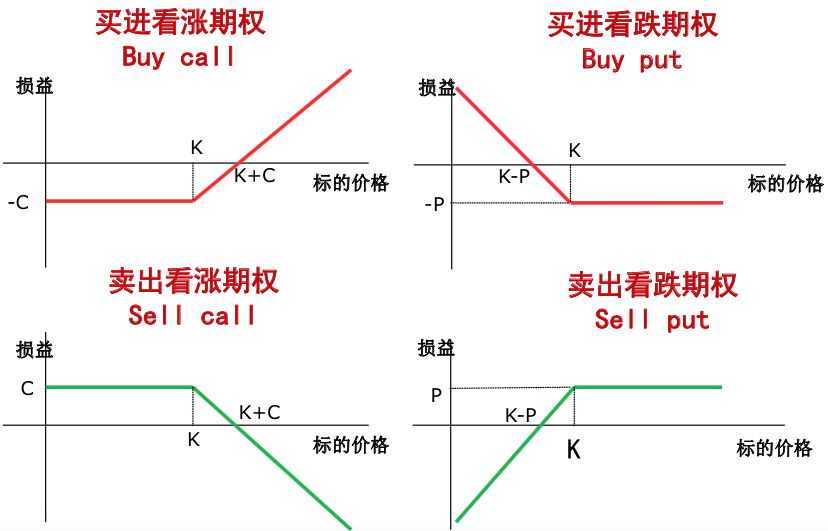
\includegraphics[width=0.8\textwidth]{fig/options-maturity-profit.png}
    \caption{期权到期收益}
    \label{fig:options-maturity-profit}
\end{figure}

\subsubsection*{术语}

\begin{itemize}
    \item Option Type:指看涨或看跌期权
    \item Option Style:指欧式期权或美式期权
    \item Option Chain:相同标的,所有的看涨期权\uline{和}所有看跌期权(即所有期权)
    \item Option Class:相同标的,所有的看涨期权\uline{或}所有看跌期权(即所有相同Option Type的期权)
    \item Option Series:相同标的,相同行权价、相同\uline{到期月份}的所有的看涨期权\uline{或}所有看跌期权
\end{itemize}

以Option Series为例,可以看到相同标的百度、相同到期月份为3月、相同行权价为80的有3个,分别为如下所示,其中除了前四位为标的,接下去的六位为YYMMDD,此时可以看到,在三月到期的有3月16日,3月22日与3月28日三个期权,其中16号为Quarterlly option,而22号为Weekly option,28号为由于周五为Easter friday,那么就移动到最近的交易日为周四:
\begin{itemize}
    \item BIDU130316C00080000
    \item BIDU130322C00080000
    \item BIDU130328C00080000
\end{itemize}

\begin{figure}[H]
    \centering
    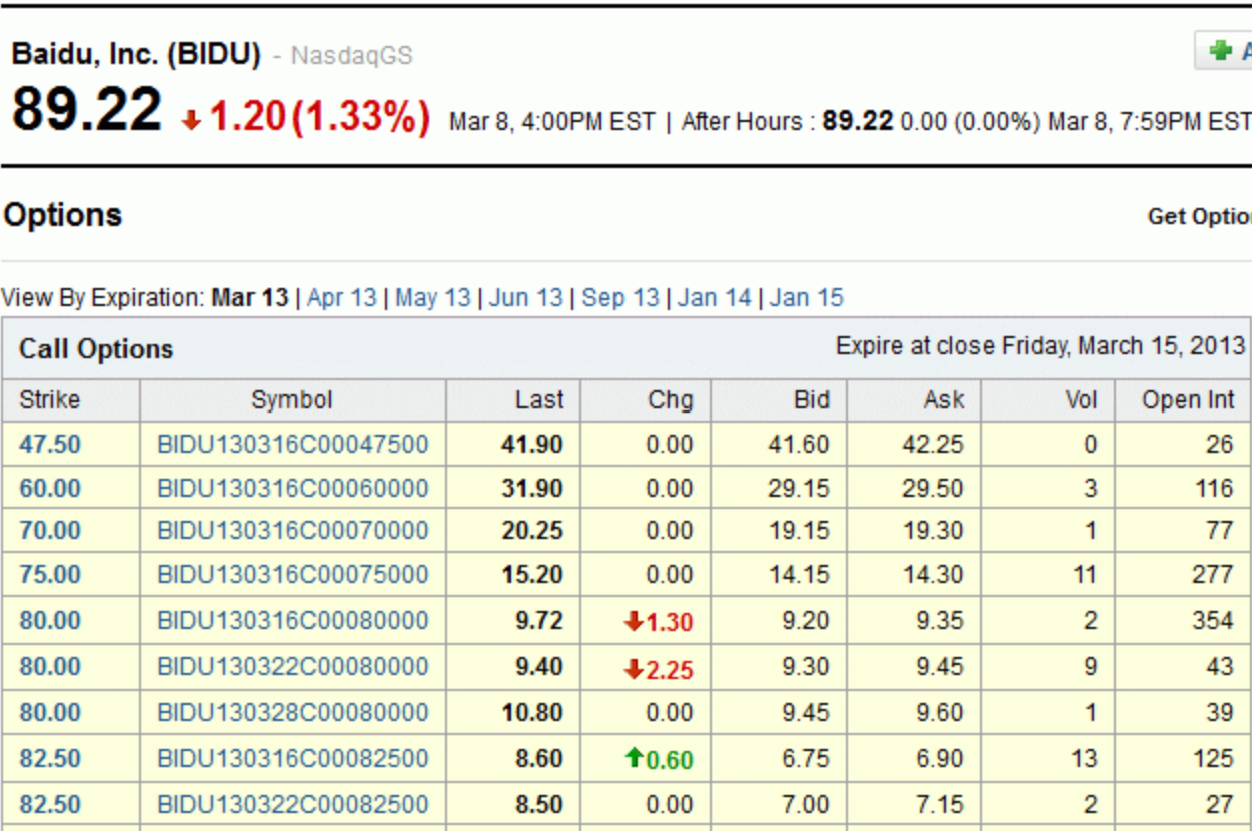
\includegraphics[width=0.8\textwidth]{fig/option-series.png}
    \caption{Option Series}
    \label{fig:option-series}
\end{figure}

\section{布朗运动与维纳过程}

\textbf{布朗运动}(Brownian motion)指是微小粒子或者颗粒在流体中做无规则运动。在数学中将这种运动定义为\textbf{维纳过程}(Wiener process)是一种连续时间随机过程,为描述证券价格随机性的基本模型,而对于期权以及其他的金融衍生品则可认为是证券价格的函数,此时衍生品价格为证券价格这一随机过程的函数。即只需要假定标的资产遵循的随机过程,利用伊藤引理可得到衍生品遵循随机过程,使得我们可以利用随机分析(Stochastic calculus)这一工具,对期权以及其他金融衍生品的价格进行量化建模。早在1900年法国人路易斯 • 巴舍利耶(Louis Bachelier)在他的博士论文《投机理论》(Théorie de la spéculation)中首次使用随机过程(现称布朗运动)分析股票和期权的价格。比爱因斯坦于1905年提出的描述花粉粒子在水中运动的论文提早了5年。

标准布朗运动(Standard Brownian motion)简易表达式(连续形式)有,其中$\varepsilon \sim N(0,1)$:
\begin{equation*}
    dW_t = \varepsilon_t \sqrt{dt}
\end{equation*}

离散形式有:
\begin{equation*}
    W_T - W_t = \sum^n_{i=1} \varepsilon_i \sqrt{\Delta t}
\end{equation*}

\subsection{特征}

布朗运动或维纳过程,为定义在非负时域t上连续随机过程。虽然连续但其\textbf{处处不可微分},其特征有:
\begin{itemize}
    \item 初值为零
    \item 独立增量:对于任意两个不同时间点$\Delta t_i$与$\Delta t_j$,其增量$\Delta W_i$与$\Delta W_j$相互独立
    \item 平稳性:增量$\Delta W$服从均值为零、方差等于时间长度的正态分布,即$\Delta W_i \sim N(0,\Delta t_i)$
\end{itemize}

并且由如上性质可知,布朗运动是一个马尔科夫过程(Markov process),即该过程在任意t时刻之后的位置,仅和t时刻的位置有关,与之前的历史轨迹无关。即该过程的当前值就包含了对其未来做预测所需的全部信息。并且由于其虽然连续,但处处不可微分的性质,使得几个点微积分无法使用,只能使用伊藤微积分(Itô calculus)进行运算。

\subsection{部分证明}

\textbf{增量均值为零,方差为时间长度},当$X$与$Y$独立时,则有:
\begin{equation*}
    \Var(XY) = \Var(X)\Var(Y) + [\E(X)]^2 \Var(Y) + [E(Y)]^2 \Var(X)
\end{equation*}

此时,由于$\varepsilon_t$与$dt$独立,套用上式,同时由于$\varepsilon_t \sim N(0,1)$,则有:
\begin{equation*}
    \E(dZ_t) = \E(\varepsilon_t \sqrt{dt}) = 0
\end{equation*}

应为方差有:
\begin{align*}
    \Var(dZ_t) & = \Var( \varepsilon_t \sqrt{dt}) \\
    & =  \Var(\varepsilon_t) \Var(\sqrt{dt}) + [\E(\varepsilon_t)]^2 \Var(\sqrt{dt}) + [E(\sqrt{dt})]^2 \Var(\varepsilon_t) \\
    & = \Var(\varepsilon_t) \left[ \Var[(\sqrt{dt})^2] - [\E(\sqrt{dt})]^2 \right] \\
    & = \Var(\varepsilon_t) \left[ \E[(\sqrt{dt})^2] - [\E(\sqrt{dt})]^2 + [\E(\sqrt{dt})]^2 \right] \\
    & = 1 \cdot \E(dt) = dt
\end{align*}

\textbf{方差可加性},由下式可见,由于独立增量,导致协方差项为零,使得方差可加。
\begin{align*}
     & \Var(X_1+X_2+X_3) \\
     & = \Var(X_1) + \Var(X_2) + \Var(X_3) \\
     & + \Cov(X_1,X_2) + \Cov(X_2,X_3) + \Cov(X_1,X_3)
\end{align*}

由上可知,增量在连续形式$dW_t$以及离散形式$W_T-W_t$下,均服从均值为零,方差为时间长度的正态分布,即有:
\begin{align*}
    dW_t & \sim N(0,dt) \\
    W_T - W_t & \sim N(0,T-t)
\end{align*}

\subsection{二次变差}

考虑区间$[0,T]$,定义$\Pi=\{0=t_0<t_1<t_2<\dots<t_N=T\}$和最大步幅$\norm{\Pi} = \max\limits_{i}(t_{i+1}-t_{i})$。为方便后续推导,假设步幅相同,即$t_{i+1} - t_{i} = \tfrac{T}{n}$。$s_i \in (t_i,t_{i+1})$,则有对于任意一个连续函数$f(t)$,其二次变差(Quadratic variation)定义为:
\begin{equation*}
    \sum^{N-1}_{i=0} \left[ f(t_{i+1} - f(t_i)) \right]^2
\end{equation*}

对于一个连续且在$[0,T]$中处处可微的函数$f(t)$,$t_{i^*} \in [t_{i},t_{i+1}]$,利用微分中值定理,可以看到随着时间的越来越细的划分,$\norm{\Pi}$趋近于零。则可得到处处可微的连续函数,在区间$[0,T]$的二次变分为0。
\begin{align*}
    \sum_{i=0}^{N-1} \left[ f(t_{i+1}) -f(t_{i}) \right]^2 
    &= \sum_{i=0}^{N-1} f'(t_{i^*})^2 (t_{i+1} - t_{i})^2 \\
    &= \norm{\Pi} \sum_{i=0}^{N-1} f'(t_{i^*})^2 (t_{i+1} - t_{i})
\end{align*}

于是有:
\begin{align*}
    [f,f](T) &= \lim\limits_{\norm{\Pi} \rightarrow 0} \norm{\Pi} \left[ \sum_{i=0}^{N-1} f'(t_{i^*})^2 (t_{i+1} - t_{i}) \right] \\
    &= \lim\limits_{\norm{\Pi} \rightarrow 0} \norm{\Pi} \cdot \lim\limits_{\norm{\Pi} \rightarrow 0} \sum_{i=0}^{N-1} f'(t_{i^*})^2 (t_{i+1} - t_{i}) \\
    &= \lim\limits_{\norm{\Pi} \rightarrow 0} \norm{\Pi} \cdot \int^T_0 f'(t_{i^*})^2 dt = 0
\end{align*}

证明需要假设$\int^T_0 f'(t_{i^*})^2 dt$为有限,如果为无限则会出现$0\cdot \infty$的情形。

\begin{thm}
    设$\Pi=\{0=t_0<t_1<t_2<\dots<t_N=T\}$为$[0,T]$的分划。布朗运动对应的样本二次变差有:
    \begin{align*}
        Q_{\Pi} = \sum_{i=0}^{N-1} \left[ W(t_{i+1}) - W(t_{i}) \right]^2 = T \qquad \text{almost surely.}
    \end{align*}
\end{thm}

\begin{proof}
    样本二次变差为独立随机变量所组成,因此其均值为这些随机变量的均值,方差为这些随机变量方差之和。并且有$\Var X = \E X^2 - \E^2 X $:
    \begin{equation*}
        \E [(W(t_{i+1}) - W(t_{i}))^2] = \Var [W(t_{i+1}) - W(t_{i})] + \E^2 [W(t_{i+1}) - W(t_{i})]= t_{i+1} - t_{i}
    \end{equation*}

    由此可以得到:
    \begin{equation*}
        \lim\limits_{\norm{\Pi} \rightarrow 0} \E(Q_{\Pi})
        = \sum_{i=0}^{N-1} \E \left[(W(t_{i+1}) - W(t_{i}))^2 \right]
        =  \sum_{i=0}^{N-1} (t_{i+1} - t_{i}) = T
    \end{equation*}

    对于方差,应有:
    \begin{equation*}
        \Var [(W(t_{i+1}) - W(t_{i}))^2] = \E [(W(t_{i+1}) - W(t_{i}))^4] - \E^2 [(W(t_{i+1}) - W(t_{i}))^2]
    \end{equation*}

    对于四次方项$\E [(W(t_{i+1}) - W(t_{i}))^4]$,可通过对正态分布矩母函数$M_X(t)$对$t$不断求导得到其期望,需求四阶导数$M_X^{(4)}(t)$:
    \begin{align*}
        M_X(t) &= \E(e^{xt}) = e^{\mu t + \frac{1}{2} \sigma^2 t^2} \\
        M'_X(t) &= (\mu + \sigma^2 t)e^{\mu t + \frac{1}{2} \sigma^2 t^2} \\
        M''_X(t) &= (\mu^2 + 2 \mu \sigma^2 t + \sigma^4 t^2 + \sigma^2)e^{\mu t +\frac{1}{2} \sigma^2 t^2} \\
        M^{(3)}_X(t) &= (\mu^3 + 3 \mu^2 \sigma^2 t + 3\mu \sigma^4 t^2 + 3\mu \sigma^2 + \sigma^6 t^3 + 3\sigma^4 t)e^{\mu t +\frac{1}{2} \sigma^2 t^2} \\
        M^{(4)}_X(t) &= (\mu^4 + 4 \mu^3 \sigma^2 t + 6 \mu^2 \sigma^4 t^2 + 6\mu^2 \sigma^2 + 4\mu\sigma^6 t^3 \\
        &\qquad + 12\mu\sigma^4 t + \sigma^8 t^4 + 6\sigma^6 t^2 + 3\sigma^4)e^{\mu t +\frac{1}{2} \sigma^2 t^2}
    \end{align*}

    因为$W(t_{i+1}) - W(t_{i}) \sim N(0,t_{i+1}-t_{i})$,其均值$\mu=0$计算四阶中心矩$M_X^{(4)}(0) = 3\sigma^2$,令$t=0$:
    \begin{equation*}
        \E [(W(t_{i+1}) - W(t_{i}))^4] = 3(t_{i+1}-t_{i})^2 
    \end{equation*}

    因此可继续计算单个时间间隔的方差:
    \begin{align*}
        \Var [(W(t_{i+1}) - W(t_{i}))^2] &= \E [(W(t_{i+1}) - W(t_{i}))^4] - \E^2 [(W(t_{i+1}) - W(t_{i}))^2] \\
        &= 3(t_{i+1}-t_{i})^2 - (t_{i+1}-t_{i})^2 \\
        &= 2(t_{i+1}-t_{i})^2
    \end{align*}

    因此在$[0,T]$的方差为:
    \begin{align*}
        \Var(Q_{\Pi}) &= \sum_{i=0}^{N-1} \Var \left[(W(t_{i+1}) - W(t_{i}))^2 \right] \\
        &=  \sum_{i=0}^{N-1} 2(t_{i+1}-t_{i})^2
        \leq \sum_{i=0}^{N-1} 2\norm{\Pi} (t_{i+1}-t_{i}) \\
        &= 2\norm{\Pi} \sum_{i=0}^{N-1} (t_{i+1}-t_{i}) \\
        &= 2\norm{\Pi} T
    \end{align*}

    由此可知当最大步幅$\norm{\Pi}$趋近于零时,方差也将趋近于零:
    \begin{align*}
        \lim\limits_{\norm{\Pi} \rightarrow 0} \Var(Q_{\Pi}) = 0
    \end{align*}

    利用切比雪夫不等式(Chebyshev's inequality):
    \begin{align*}
        P\left( \abs{Q_{\Pi} - \E(Q_{\Pi}} \geq \frac{1}{n} \right) &\leq n^2 \Var(Q_{\Pi}) \\
        \lim_{\norm{\Pi} \rightarrow 0} P\left( \abs{Q_{\Pi} - T} \geq \frac{1}{n} \right) &\leq n^2 \lim_{\norm{\Pi} \rightarrow 0} \Var(Q_{\Pi})  \\
        \lim_{\norm{\Pi} \rightarrow 0} P\left( \abs{Q_{\Pi} - T} \geq \frac{1}{n} \right) &= 0
    \end{align*}
    
    因此在概率上几乎必然成立,即虽然有可能存在某些布朗运动使得其二次变差为T不成立,但这样的情形概率为0:
    \begin{equation*}
        \lim_{\norm{\Pi} \rightarrow 0} Q_{\Pi} = \E Q_\Pi = T
    \end{equation*}
\end{proof}

可以看到而对于布朗运动$B(t)$,虽然连续但处处不可微分,使得其无法像其他连续可微分函数一样计算二次变差。其非零的二次变分说明随机性使得它的波动太频繁,以至于不管我们如何细分区间、得到多么微小的划分区间T,累加这些微小区间上的变化总和,二次变分都不会消失(即二次变分不为0),而是等于这个区间的长度T。布朗运动的二次变差可简写为无穷小量,为$(dB)^2=dt$。其中无穷小量在英文中应为differential或infinitesimal difference,其中infinitesimal即infinitely small。

\subsection{几种随机过程}

\textbf{广义维纳过程}(generalized Wiener process),a与b为常数。此时,易知其均值为$\E(dX_t) = adt$,由于$b$为常数,且$\Var(dW_t)=dt$,则有方差为$\Var(dX_t)=b^2 dt$。
\begin{equation*}
    dX_t = a dt + b dW_t
\end{equation*}

\textbf{普通布朗运动},a(t)与b(t)都是t的确定性函数。由于都为确定函数,所以如上可知,其均值方差为$\E(dX_t) = a(t)dt$,由于$b$为常数,且$\Var(dW_t)=dt$,则有方差为$\Var(dX_t)=b(t)^2 dt$。
\begin{equation*}
    dX_t = a(t) dt + b(t) dW_t
\end{equation*}

\textbf{伊藤扩散过程}(Itô diffusion),此时$a(X(t),t)$与$b(X(t),t)$都为$X_t$和$t$的确定性函数。由于漂移项与方差项都包含$X(t)$,使得扩散之后过程的条件分布无法保证仍是正态分布。但更能刻画一般动态变化,未加入新的风险源,仍具有独立增量,马尔可夫性,和方差可加性等性质。
\begin{equation*}
    dX_t =a(X(t),t) dt + b(X(t),t) dW_t
\end{equation*}

以上都为\textbf{随机微分方程}(Stochastic differential equation,SDE),与普通微分方程的延伸,特指的是包含随机过程的微分方程。\textbf{注意}:虽然$B(t)$处处不可微,单$dB(t)$指布朗运动在一个无限小的时间间隔内的变化。

\section{伊藤引理}

\subsection{古典微积分为何失效}

有了随机过程$X_t$或维纳过程$W_t$,由于衍生品价格是标的资产价格$S_t$与时间$t$的函数。我们就需要进一步研究随机过程的函数,研究$f$在无穷小的时间间隔内的变化,即$df(\cdot)$。由上在分析二次变差可以发现,由于布朗运动处处不可微的性质,使得古典微积分无法适用于随机过程。日本数学家伊藤清(Itō Kiyoshi)提出伊藤微积分解决了这一问题。

对于古典的微积分中的链式法则,由于布朗运动处处不可微分,即$dW_t/dt$不存在,使得等式无意义。
\begin{equation*}
    \frac{df(W_t)}{dt} = f'(W_t)\frac{dW_t}{dt}
\end{equation*}

对于函数$f(x)$使用泰勒展开,应有:
\begin{equation*}
    f(x + \Delta x) - f(x)= f'(x)(\Delta x) + \frac{1}{2} f''(x)(\Delta x)^2 + \frac{1}{6} f'''(x)(\Delta x)^3 + \dots
\end{equation*}

对于普通变量$X$,可以发现当$\Delta x$趋近于$0$时,除了第一项,其他项都为高阶小量,因此均可被忽略,因此其无穷小量形式应为$df=f'(x)dx$。而对于随机变量$W_t$,进行泰勒展开:
\begin{equation*}
    df = f(W_t + \Delta W_t) - f(W_t)= f'(W_t)(\Delta W_t) + \frac{1}{2} f''(W_t)(\Delta W_t)^2 + \frac{1}{6} f'''(W_t)(\Delta W_t)^3 + \dots
\end{equation*}

与普通随机变量相同的是第一项需要保留,但第二项对于普通随机变量来说已经是高阶小量了,但对于随机过程变量$W_t$,已知其二次变差为$(dW_t)^2 = dt$,与第一项为同阶,不能忽略。而从第三项开始之后的所有项才可以被忽略,因此得到伊藤引理的最基本形式:
\begin{equation*}
    df(W_t) =f'(W_t)dW_t + \frac{1}{2}f''(W_t)dt
\end{equation*}

\subsection{伊藤引理与证明}

\begin{lemma}
    伊藤引理(Itô lemma),假设变量$X_t$遵循如下随机过程:
    \begin{equation*}
        dX_t =\mu_t dt + \sigma_t dW_t
    \end{equation*}

    在导数$\dfrac{\partial f}{\partial t}$、$\dfrac{\partial f}{\partial X}$与$\dfrac{\partial^2 f}{\partial X^2}$存在的前提下,则有变量$X_t$和$t$的函数$f(X(t),t)$将遵循如下过程:
    \begin{equation*}
        df(X_t,t) = \left(\frac{\partial f}{\partial t} + \mu_t \frac{\partial f}{\partial x} + \frac{1}{2} \sigma_t^2 \frac{\partial^2 f}{\partial x^2} \right)dt + \sigma_t \frac{\partial f}{\partial X} dW_t
    \end{equation*}
\end{lemma}

\begin{proof}
    $f(X,t)$的泰勒展开式为:
    \begin{equation*}
        \Delta f_t = \frac{\partial f}{\partial X} \Delta X + \frac{\partial f}{\partial t} \Delta t + \frac{1}{2} \frac{\partial^2 f}{\partial X^2}\Delta X^2  + \frac{\partial f}{\partial X \partial t}\Delta X \Delta t + \frac{1}{2} \frac{\partial^2 f}{\partial t^2} \Delta t^2 + \dots
    \end{equation*}

    当$\Delta t \rightarrow 0$时,$(\Delta t)^2$,认为是高阶无穷小,可忽略。而对于$\Delta X \Delta t$项有:
    \begin{align*}
        \Delta X &= a\Delta t + b \varepsilon\sqrt{\Delta t} \\
        \Delta X \Delta t &= a(\Delta t)^2 + b \varepsilon(\Delta t)^{3/2}
    \end{align*}

    其中的$(\Delta t)^{3/2}$项,也被认为时高阶无穷小项,可忽略。同时由于$(\Delta X)^2$项中包含$\Delta t$项,因此需要保留。仅考虑前三项,展开得到:
    \begin{align*}
        \Delta f_t & = \frac{\partial f}{\partial X} \Delta X + \frac{\partial f}{\partial t} \Delta t + \frac{1}{2} \frac{\partial^2 f}{\partial X^2}\Delta X^2 \\
        & = \frac{\partial f}{\partial X} \Delta X + \frac{\partial f}{\partial t} \Delta t + \frac{1}{2} \frac{\partial^2 f}{\partial X^2} [a\Delta t + b\varepsilon\sqrt{\Delta t}]^2 \\
        & = \frac{\partial f}{\partial X} \Delta X + \frac{\partial f}{\partial t} \Delta t + \frac{1}{2} \frac{\partial^2 f}{\partial X^2} b^2 \varepsilon^2 \Delta t
    \end{align*}

    对于$\varepsilon^2 \Delta t$项,由于$\varepsilon \sim N(0,1)$,因此有$\E(\varepsilon)=0$。又因$\Var(\varepsilon)=\E(\varepsilon^2)-[\E(\varepsilon)]^2=1$,得到$\E(\varepsilon^2)=1$,同时有$\E(\varepsilon^2 \Delta t) = \Delta t$。计算$\varepsilon^2 \Delta t$的方差可得:
    \begin{align*}
        \Var(\varepsilon^2 \Delta t) & = \Var(\varepsilon^2) \Var(\Delta t) + [\E(\varepsilon^2)]^2 \Var(\Delta t) + [E(\Delta t)]^2 \Var(\varepsilon^2) \\
        & = \Var(\varepsilon^2) \Var(\Delta t) + 1 \cdot \Var(\Delta t) + [E(\Delta t)]^2 \Var(\varepsilon_t^2) \\
        & = \mathcal{O}(\Delta t^2)
    \end{align*}

    可以认为$\varepsilon^2 \Delta t$方差为高阶无穷小,其期望为$1$。因此,可认为$\varepsilon^2 \Delta t \approx \Delta t$,可将原式化简为:
    \begin{equation*}
        \Delta f_t = \frac{\partial f}{\partial X} \Delta X + \frac{\partial f}{\partial t} \Delta t + \frac{1}{2} \frac{\partial^2 f}{\partial X^2} b^2 \Delta t
    \end{equation*}

    而连续形式为:
    \begin{align*}
        df_t & = \frac{\partial f}{\partial X}  dX_t + \frac{\partial f}{\partial t} dt + \frac{1}{2} \frac{\partial^2 f}{\partial X^2} b^2 dt \\
        & = \frac{\partial f}{\partial X} (a_t dt + b_t dW_t) + \frac{\partial f}{\partial t} dt + \frac{1}{2} \frac{\partial^2 f}{\partial X^2} b^2 dt \\
        & = \left(\frac{\partial f}{\partial X}a_t  + \frac{\partial f}{\partial t} + \frac{1}{2}\frac{\partial^2 f}{\partial X^2} b^2_t \right)dt + \frac{\partial f}{\partial X} b_t dW_t
    \end{align*}
\end{proof}

由此可知,$f$作为随机过程$X$与时间$t$的函数,其本身也是一个随机过程。而$df_t$与$dX_t$的随机性\textbf{来源于同一布朗运动}$dW_t$,而非两个独立的布朗运动。为方便记忆,可记为(金融随机分析第二卷 P118):
\begin{equation*}
    \boxed{
        df(X(t),t) = f_t(X(t),t)dt + f_x(X(t),t)dX(t) + \frac{1}{2}f_{xx}(X(t),t)dX(t)dX(t)
    }
\end{equation*}

或可写为更简洁的形式:
\begin{equation*}
    \boxed{
        df = f_t dt + f_x dX + \frac{1}{2}f_{xx}dXdX
    }
\end{equation*}

\section{几何布朗运动}

由上可知随机过程$X(t)$随着时间$t$的变化,可能为负数,但股票价格显然不可能为负。收益率却有正有负,因此可以使用$X(t)$来描绘收益率。假设$S_t$为股票价格,可以假设其百分比收益率遵循如下随机过程:
\begin{equation*}
    \frac{dS_t}{S_t} = \mu dt + \sigma dW_t
\end{equation*}

因此$S_t$的随机微分形式如下,此时股票价格$S_t$服从\textbf{几何布朗运动}(Geometric Brownian Motion,GBM):
\begin{equation*}
    dS_t = \mu S_t dt + \sigma S_t dW_t
\end{equation*}

令$f(S_t) = \ln S_t$,此时:
\begin{equation*}
    \frac{\partial f}{\partial S} = \frac{1}{S_t}, \quad
    \frac{\partial^2 f}{\partial S^2} = -\frac{1}{S_t^2}, \quad
    \frac{\partial f}{\partial t} = 0
\end{equation*}

代入伊藤引理之中,此时$a_t=\mu S_t$,$b_t=\sigma S_t$,则有:
\begin{align*}
    df_t = d \ln S_t & = \left( \frac{1}{S_t}\mu S_t + 0 - \frac{1}{2} \frac{1}{S_t^2} \sigma^2 S_t^2 \right) dt + \frac{1}{S_t}\sigma S_t dW_t \\
    & = \left( \mu - \frac{1}{2}\sigma^2\right)dt + \sigma dW_t
\end{align*}

连续形式下有:
\begin{equation*}
    d\ln S = \left( \mu - \frac{1}{2}\sigma^2\right) dt + \sigma dW_t \sim N \left( (\mu-\frac{\sigma^2}{2})dt, \sigma^2 dt \right)
\end{equation*}

离散形式下为:
\begin{align*}
    \Delta \ln S &= \ln S_T - \ln S_t = \left( \mu - \frac{\sigma^2}{2} \right) \Delta t + \sigma (W_T - W_t) \\
    \Delta \ln S &\sim N \left((\mu-\frac{\sigma^2}{2})(T-t), \sigma^2(T-t) \right)
\end{align*}

可以看到\textbf{连续复合收益率}或\textbf{对数收益率}服从期望值为$(\mu - \tfrac{\sigma^2}{2})dt$,方差为$\sigma^2 dt$的\textbf{正态分布},与现实较为吻合。且$d\ln S_t$的定义,使得股票价格非负。对于日频收益率的计算,此时得到的正态分布均值以及方差均为日频($T-t=\frac{1}{252}$),需乘以252进行年化,得到年化的收益率均值与波动率。在$T$时刻,\textbf{股票价格的对数}($\ln S$),也服从\textbf{正态分布},则有\textbf{股票价格}($S$)服从\textbf{对数正态分布}。
\begin{equation*}
    \ln S_T  \sim N \left(\ln S_t + (\mu-\frac{\sigma^2}{2})(T-t), \sigma^2(T-t)\right)
\end{equation*}

可以看到选择几何布朗运动描绘股票价格$S_t$有如下几大优点:
\begin{itemize}[leftmargin=4em]
    \item 正态分布:经验事实证明,股票价格的连续复合收益率,近似地服从正态分布
    \item 马尔科夫过程:由布朗运动的性质可知,利用几何布朗运动描绘的股票价格是一个马尔科夫过程,即当前价格就包含了对其未来做预测所需的全部信息,这与弱有效市场假说相符
    \item 布朗运动在时间上处处不可微以及二次变分不为零的性质符合股票收益率在时间上存在转折尖点的特征。
\end{itemize}

\section{对数正态分布}

由\textbf{股票价格的对数}服从\textbf{正态分布}可知,股票价格应服从\textbf{对数正态分布}(Log-normal distribution)。由正态分布与对数正态分布的性质可知,对一个服从正态分布的随机变量$X$取指数,则$e^X$服从对数正态分布。相反,对一个服从对数正态分布的随机变量$X$取对数,则$\ln X$服从正态分布(因而得名,取对数得到正态分布的分布)。因此有如下关系:
\begin{align*}
    \ln S_T \sim N(\mu,\sigma^2) \quad \leftrightarrow \quad S_T \sim \text{Log-normal}(\mu,\sigma^2)
\end{align*}

对于对数正态分布$X \sim \text{Log-normal}(\mu,\sigma^2)$,其期望与标准差为:
\begin{align*}
    \E(X) & = e^{\mu+\frac{\sigma^2}{2}} \\
    \Var(X) & = e^{2\mu+\sigma^2} (e^{\sigma^2}-1)
\end{align*}

已知股票价格的对数$\ln S_T$服从如下正态分布:
\begin{equation*}
    \ln S_T  \sim N \left(\ln S_t + (\mu-\frac{\sigma^2}{2})(T-t), \sigma^2(T-t)\right)
\end{equation*}

那么股票价格$S_T$服从如下对数正态分布:
\begin{equation*}
    S_T  \sim \text{Log-normal} \left(\ln S_t + (\mu-\frac{\sigma^2}{2})(T-t), \sigma^2(T-t)\right)
\end{equation*}

可求得股票价格得期望与方差为:
\begin{align*}
    \E(S_T)   & = \exp\left( \ln S_t + (\mu - \frac{\sigma^2}{2})(T-t)+\frac{\sigma^2(T-t)}{2}\right) \\
    & = \exp \left( \ln S_t + \mu(T-t) \right) \\
    & = S_t e^{\mu(T-t)} \\
    \Var(S_T) & = \left[\exp(\sigma^2(T-t))-1\right] \exp \left\{2\left[\ln S_t + (\mu - \frac{\sigma^2}{2})(T-t)\right] + \sigma^2(T-t)\right\} \\
    & = \left[\exp(\sigma^2(T-t))-1\right] \exp\left[2 \ln S_t + 2\mu (T-t)\right] \\
    & = S_t^2 e^{2\mu(T-t)} \left[ e^{\sigma^2 (T-t)} - 1 \right]
\end{align*}

\subsection*{注意}

对于正态分布只需要$\mu$与$\sigma$两个参数即可确定其分布,同时$\mu$与$\sigma^2$也是正态分布的均值与方差。对于对数正态分布,也仅需要$\mu$与$\sigma$两个参数便可确定其分布,但并非其均值与方差。对于相同的$\mu$与$\sigma$参数确定的正态分布与对数正态分布,两者之间的期望与方差通过如下表格关系转化:
\begin{table}[H]
\centering
\begin{tabular}{@{}cll@{}}
\toprule
\multicolumn{1}{l}{}
& \multicolumn{1}{c}{\textbf{正态分布}$\quad N \sim (\mu,\sigma)$} & \multicolumn{1}{c}{\textbf{对数正态分布}$\quad logN \sim (\mu,\sigma)$} \\
\midrule
\multirow{1}{*}{\textbf{期望}} 
& $\E_N(X) \equiv \mu = \ln[\E_{L}(X)] - \frac{1}{2} \ln \left[1+\frac{\Var_{L}(X)}{[\E_{L}(X)]^2}\right] $ & $\E_{L}(X) = e^{\mu+\frac{1}{2}\sigma^2}$ \\
\textbf{方差} & $\Var_N(X) \equiv \sigma^2 = \ln \left[1+\frac{\Var_{L}(X)}{[\E_{L}(X)]^2}\right]$ & $\Var_{L}(X) = e^{2\mu+\sigma^2} 
\left(e^{\sigma^2} - 1\right)$ \\
\bottomrule
\end{tabular}
\end{table}

\subsection{PDF与CDF}

如下图所示,通过对服从\textbf{正态分布}的随机变量\textbf{取指数},可以将其转换为对数正态分布。同理,通过对服从\textbf{对数正态分布}的随机变量\textbf{取对数},使其转换为正态分布。假设随机变量$Y \sim N(\mu,\sigma^2)$ 服从正态分布,随机变量$X \sim \text{Log}N(\mu,\sigma^2)$,对正态分布随机变量$Y$取指数$x=e^y$,此时有$y = \ln x$,带入CDF中,可得到对数正态函数CDF。对两者求导,可得PDF函数。
\begin{table}[H]
\centering
\begin{tabular}{@{}cll@{}}
\toprule
\multicolumn{1}{l}{}
& \multicolumn{1}{c}{\textbf{正态分布}} & \multicolumn{1}{c}{\textbf{对数正态分布}} \\
\midrule
\multirow{1}{*}{\textbf{PDF}} 
& $\frac{1}{\sigma\sqrt{2\pi}} e^{-\frac{1}{2} \left( \frac{x-\mu}{\sigma} \right)^2 } $
& $\frac{1}{x\sigma\sqrt{2\pi}} e^{-\frac{1}{2} \left( \frac{\ln x-\mu}{\sigma} \right)^2 } $ \\
\textbf{CDF} 
& $\frac{1}{2} \left[1 + \text{erf}\left( \frac{x-\mu}{\sigma\sqrt{2}}\right) \right]$
& $\frac{1}{2} \left[1 + \text{erf}\left( \frac{\ln x-\mu}{\sigma\sqrt{2}}\right) \right]$ \\
\bottomrule
\end{tabular}
\end{table}

\begin{figure}[H]
    \centering
    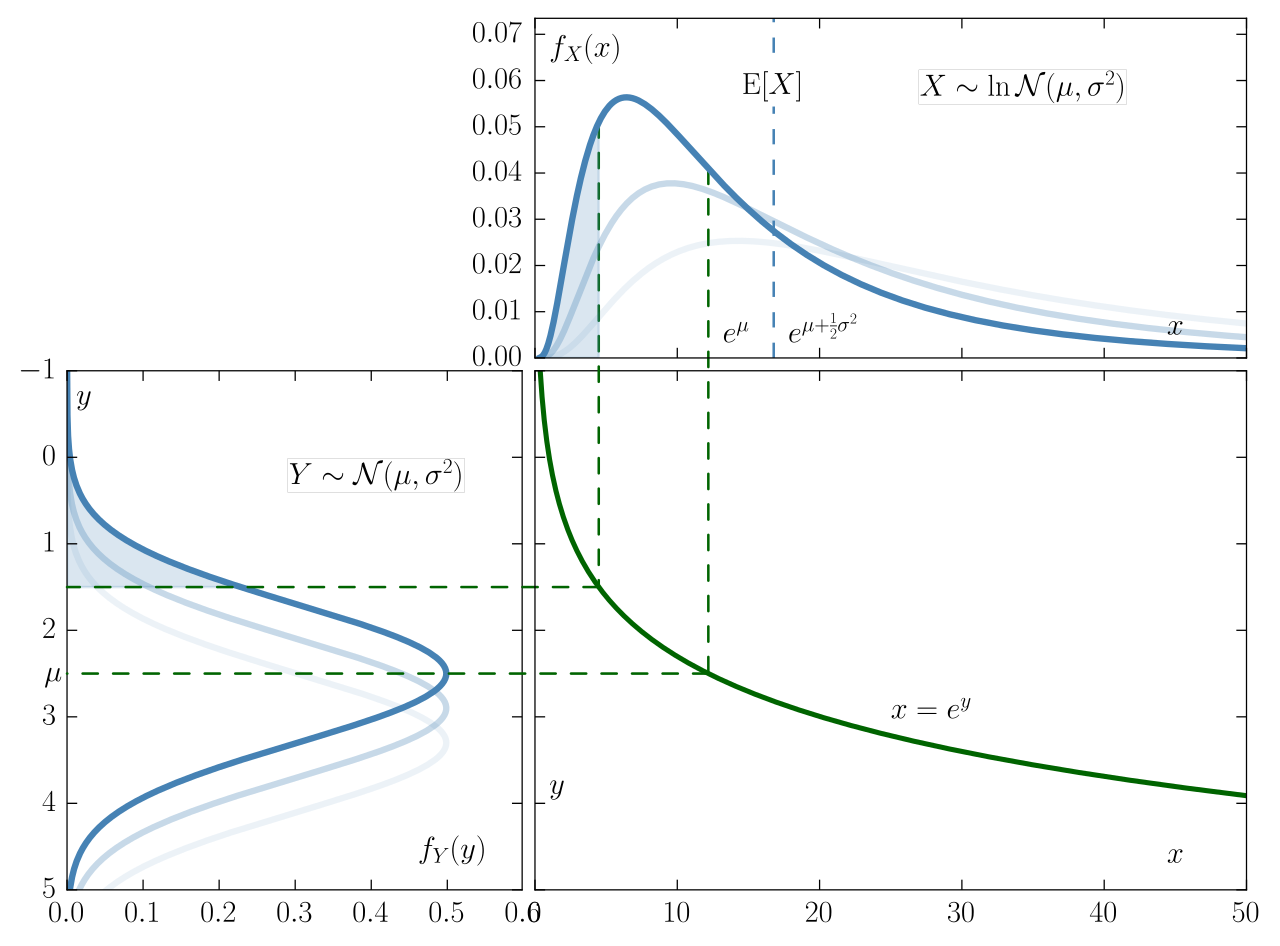
\includegraphics[width=0.9\textwidth]{fig/lognormal-distribution.png}
    \caption{两者相互转换}
    \label{fig:lognormal}
\end{figure}

\subsection{PDF推导}

如上文所述,对于相同参数$\mu$与$\sigma^2$的正态分布与对数正态分布可以相互转化。两者互相经过转化后,其累积分布函数(Cumulative distribution fuction,CDF)相同。如图\ref{fig:lognormal}所示,假设随机变量$Y \sim N(\mu,\sigma^2)$ 服从正态分布,随机变量$X \sim \text{Log}N(\mu,\sigma^2)$,则应有如下关系,对服从对数正态分布的随机变量$X$取对数,使其转化为正态分布:
\begin{equation*}
    \text{CDF}_{logN}(x) = \text{CDF}_N (\ln x) = \text{CDF}_N (y)
\end{equation*}

对公式两边取导数,则可得到其概率密度函数(Probability density function,PDF):
\begin{equation*}
    \text{PDF}_{logN}(x) = \frac{1}{y} \text{PDF}_N(\ln x)
\end{equation*}

此时,带入已知正态分布PDF,即可得到对数正态分布PDF:
\begin{equation*}
    \text{PDF}_{logN} = \frac{1}{x\sigma\sqrt{2\pi}} e^{-\frac{(\ln x - \mu)^2}{2\sigma^2}}
\end{equation*}

\subsubsection{期望推导}

根据对数正态分布的PDF,可计算其期望:
\begin{equation*}
    \E(X) = \int^{+\infty}_0 x f(x) dx = \int^{+\infty}_0 \frac{1}{\sigma\sqrt{2\pi}} e^{-\frac{(ln x - \mu)^2}{2\sigma^2}} dx
\end{equation*}

使用换元法,令$t = \frac{\ln x - \mu}{\sqrt{2}\sigma}$,则有$x = e^{\sqrt{2}\sigma t + \mu}$,则原积分转化为:
\begin{align*}
    \E(X) &= \int^{+\infty}_{-\infty} \frac{1}{\sigma\sqrt{2\pi}}e^{-t^2}d e^{\sqrt{2}\sigma t + \mu}\\ 
    &= \frac{e^{\mu + \frac{\sigma^2}{2}}}{\sqrt{\pi}} \int^{+\infty}_{-\infty} e^{-(t-\frac{\sqrt{2}\sigma}{2})^2} dt\\ 
    &= \frac{e^{\mu + \frac{\sigma^2}{2}}}{\sqrt{\pi}} \int^{+\infty}_{-\infty} e^{-t^2}d e^{-(t-\frac{\sqrt{2}\sigma}{2})^2} d(t-\frac{\sqrt{2}\sigma}{2})
\end{align*}

由于$\int^{+\infty}_{-\infty} e^{x^2} = \sqrt{\pi}$,可得到:
\begin{equation*}
    \E(X) = e^{\mu+\frac{\sigma^2}{2}}
\end{equation*}

\subsubsection{方差推导}

已知:
\begin{equation*}
    \Var(X) = \E[(X-\mu)^2] = \E(X^2 -2\mu X + \mu^2) = \E(X^2) -2\mu \E(X) + \mu^{2} = \E(X^2) - [\E(X)]^2
\end{equation*}

同上,已知对数正态分布PDF:
\begin{equation*}
    \E(X^2) = \int^{+\infty}_0 x^2 f(x) dx = \int^{+\infty}_0 \frac{x}{\sigma\sqrt{2\pi}} e^{-\frac{(\ln x - \mu)^2}{2\sigma^2}} dx
\end{equation*}

使用换元法,令$t = \frac{\ln x-\mu}{\sigma}$,则有$x = e^{\sigma t + \mu}$:
\begin{align*}
    \E(X^2) &= \frac{e^{2\mu}}{\sqrt{2\pi}} \int^{+\infty }_{-\infty } e^{-\frac{t^2}{2}+2\sigma t}dt \\
    &= \frac{e^{2\mu}}{\sqrt{2\pi}} \int^{+\infty }_{-\infty } e^{-\frac{1}{2}(t-2\sigma)^2 + 2\sigma^2}dt \qquad 
    \left(\text{对}-\frac{t^2}{2}+2 \sigma t \text{配方}\right) \\
    &= \frac{e^{2\mu+2\sigma^2}}{\sqrt{2\pi}} \sqrt{2} \int^{+\infty}_{-\infty} e^{(-\frac{t-2\sigma}{\sqrt{2}})^2} d\left(\frac{t-2\sigma}{\sqrt{2}}\right)\\
    &= e^{2\mu +2\sigma^2}
\end{align*}

此时则有:
\begin{align*}
    \Var(X) &= \E(X^2) - [\E(X)]^2  \\
    &= e^{2\mu+2\sigma^2} - (e^{\mu+\frac{\sigma^2}{2}})^2 \\
    &= e^{2\mu+2\sigma^2} - e^{2\mu+\sigma^2} \\
    &= e^{2\mu+\sigma^2}\left(e^{\sigma^2} - 1\right)\\
\end{align*}

\section{比例收益率与对数收益率}

\subsection{对数收益率推导}

对数收益率,或称连续复合收益率(Continuously compounded return),以复合利率为例。假设名义利率(Nominal interest rate)为$r$,进行再投资,且一年计息$m$次,则有实际利率(Effective interest rate,EIR)为:
\begin{equation*}
    \begin{aligned}
        \text{当$m=1$时:} &\quad 1+r \\
        \text{当$m=2$时:} &\quad (1+\frac{r}{2})^2 \\
        \text{当$m=3$时:} &\quad (1+\frac{r}{3})^3 \\
        \dots &\quad \dots \\
        \text{当$m=\infty$时:} &\quad \lim_{m \rightarrow \infty} (1+\frac{r}{m})^m \\
    \end{aligned}
\end{equation*}

已知,根据定义自然常数为如下极限值:
\begin{equation*}
    e = \lim_{n \rightarrow \infty} \left(1+ \frac{1}{n}\right)^n
\end{equation*}

由下方推导可以看出,连续复合收益率为,
一段时间内,给定名义利率$r$,当计息频率无限频繁$m=\infty$时的实际利率:
\begin{equation*}
    \lim_{m \rightarrow \infty} (1+\frac{r}{m})^m = 
    \lim_{m \rightarrow \infty} (1+\frac{1}{m/r})^{\frac{m}{r} \times r} = e^r
\end{equation*}

以股票价格$S_t$为例,有对应的对数收益$R_{log}$为:
\begin{eqnarray}
    \frac{S_t}{S_{t-1}} = e^{R_{log}} \quad\rightarrow\quad R_{log} = \ln \frac{S_t}{S_{t-1}}
\end{eqnarray}

\begin{example}
    当名义利率为$12\%$时,有年化实际利率(Effective annual interest rate或Annual equivalent rate,AER)为:
    \begin{table}[H]
    \centering
    \begin{tabular}{@{}lll@{}}
    \toprule
    频率(m) & 实际利率 & 实际年化利率 \\ \midrule
    1(一年)   & $\frac{0.12}{1}=0.12$  & $(1.12)^1-1=0.12$ \\
    2(半年)   & $\frac{0.12}{2}=0.06$  & $(1.06)^2-1=0.1236$      \\
    4(季度)   & $\frac{0.12}{4}=0.03$  & $(1.03)^4-1=0.125509$       \\
    12(月度)  & $\frac{0.12}{12}=0.01$ & $(1.01)^{12}-1=0.126162$ \\
    52(周度)  & $\frac{0.12}{52}=0.0023$  & $(1.0023)^{52}-1=0.127341$\\
    365(日度) & $\frac{0.12}{365}=0.00033$ & $(1.00033)^365-1=0.127475$ \\
    $\infty$ (连续)  & \multicolumn{2}{l}{$ \lim_{m \rightarrow \infty} (1+\frac{0.12}{m})^{m} - 1 = e^{0.12} = 0.127497
    $}            \\ \bottomrule
    \end{tabular}
    \end{table}
\end{example}

\subsection{单期收益}

对于计算\textbf{单期}的收益,可分为\textbf{百分比收益}或(Arithmetic return)或称为简单收益(Simple return),与
\textbf{连续复合收益}(Continuously compounded return),或称为对数收益(Logarithmic return,或Log return)。

这里特指\textbf{收益},用记号$R$表示,而非收益率,因为收益是指单期的,而收益率则可通过对单期收益率进行年化,或对多期收益率进行平均获得。记符号$r$为收益率(Rate of return)为将一段时间的收益(Return),转化为在标准化期限内的收益。对于标准化期限为\textbf{1年}的收益率,称为年化收益率(Annulized return)。
\begin{table}[H]
\centering
\begin{tabular}{@{}cll@{}}
\toprule
\multicolumn{1}{l}{}
& \multicolumn{1}{c}{\textbf{百分比收益}} & \multicolumn{1}{c}{\textbf{对数收益}} \\
\midrule
\multirow{1}{*}{\textbf{单期}} 
& $R_{pct} = \frac{V_T}{V_t}-1$
& $R_{log} = \ln \frac{V_T}{V_t}$ \\
\bottomrule
\end{tabular}
\end{table}

由上表可知,百分比收益与对数收益有如下转换关系:
\begin{equation*}
    R_{pct} = e^{R_{log}} - 1 \quad\leftrightarrow\quad R_{log} = \ln (1+R_{pct}) 
\end{equation*}

具体而言:
\begin{equation*}
    R_{log} = \ln (1 + R_{pct}) = \ln \frac{S_t}{S_{t-1}} = \ln S_t - \ln S_{t-1}
\end{equation*}

对于投资组合$p$而言,假设其在资产$i$上的权重为$w_i$,$R_{pct,i}$为资产$i$的百分比收益,那么该投资组合其百分比收益率有:
\begin{equation*}
    R_{pct,p} = \sum_i w_i R_{pct,i}
\end{equation*}

但对于该投资组合的对数收益却没有如上性质,只有当百分比收益的的绝对值很小时,能近似的有:
\begin{equation*}
    R_{log,p} \approx \sum_i w_i R_{log,i}
\end{equation*}

\subsection{多期平均收益率}

在这里不称为收益,而称为\textbf{收益率}是因为在平均的过程中已经转化为标准化期限,即为原数据的频率,如日频的多期平均收益率,其标准化期限就为$1$天。但只有在标准化期限为年为单位是年时,才能称为是年化的收益率。

计算\textbf{多期}的平均收益率时,有\textbf{算术平均收益率}(Arithmetic mean rate of return),和\textbf{几何平均收益率}(Geometric mean rate of return)两种方式。假设共有$n$期,那么$n$期算术平均收益率有:
\begin{equation*}
    \bar{r}_{\text{算术}} = \frac{1}{n} \sum^{n}_{i=1} r_i = \frac{1}{n} (r_1 + r_2 + \dots + r_n)
\end{equation*}

$n$期几何平均收益率有:
\begin{equation*}
    \bar{r}_{\text{几何}} = \left( \prod^{n}_{i=1}(1+r_i) \right)^{\frac{1}{n}} - 1
\end{equation*}

\subsection{年化收益率}

年化即将其标准期限调整为$1$年,则称为年化收益率。单期收益可直接进行年化,而多期收益,
一般将其合并为单期收益,再根据持有资产期限长度,以年为单位进行年化(平均),最终得到年化收益率。

\subsubsection*{年化百分比收益率}

对于没有再投资(Reinvestment)的\textbf{单期}百分比收益进行年化,得到年化百分比收益率为($\tau$单位为年):
\begin{equation*}
    r_{pct} = \frac{R_{pct}}{\tau}
\end{equation*}

即如半年收益为$10\%$,则$1$年的年化为$20\%$。而对进行了再投资的,复合(Compound)百分比收益率为:
\begin{equation*}
    1+R_{pct} = (1+r_{pct})^\tau \quad\rightarrow\quad
    r_{pct} = (1+R_{pct})^{\frac{1}{\tau}} - 1
\end{equation*}

此时假设$R_{pct}$为$2$年单期收益,则$\tau = 2$,最终结果$r_{pct}$为将两年收益使用几何平均为年化百分比收益率。对于\textbf{多期}平均(几何平均)年化百分比收益率,假设R时间跨度为$1$年$k$期(若月收益,则有$k=12$),持有该资产的期限为$n$年,应有:
\begin{equation*}
    r_{pct} = \left[ \prod_{i=1}^{n\times k} (1+R_{pct,i}) \right]^{n} - 1
\end{equation*}

即先计算持有资产期限内所有收益的乘积,即为总收益,再按上述单期方法进行年化。对于单期或多期的百分比收益,都使用上式\textbf{几何平均}进行计算,得到其平均年化收益率,计算算术平均没有经济学意义。

\subsubsection*{对数收益率}

将\textbf{单期}对数收益,可以直接进行年化,可得年化对数收益率:
\begin{equation*}
    e^{r_{log}\tau} = e^{R_{log}} \quad\rightarrow\quad r_{log} = \frac{R_{log}}{\tau}
\end{equation*}

假设一支股票在一个交易日内对数收益率$R_{log}=0.14\%$,平均一年有252个交易日(每个月21个交易日),则应有年化收益率为$r_{log} = \frac{R_{log}}{1/252} = 252R_{log} = 35.28\%$。即$V_t e^{r\tau} = V_T$,那么有$r = \frac{1}{\tau} \ln \frac{V_T}{V_t}$。对于期数为$n$的\textbf{多期}对数收益率,根据其性质,只需要将每期收益相加,即可得到总收益:
\begin{align*}
    R_{log} = \sum^{n}_{i=1} R_{log,i} & = R_{log,1} + R_{log,2} + \dots + R_{log,n} \\ 
    &= \ln\frac{V_2}{V_1} + \ln\frac{V_1}{V_0} + \dots + \ln\frac{V_n}{V_{n-1}} \\
    &= \cancel{\ln V_1} - \ln V_0 + \dots + \ln V_n - \cancel{\ln V_{n-1}} \\
    &= \ln\frac{V_n}{V_0} 
\end{align*}

对于\textbf{多期}(多年)的对数收益,由于对数收益率可相加的性质,只需要计算其\textbf{算术平均},即可得到标准期限与每期期限相同的收益率,而当标准化期限为1年时得到年化对数收益率。对于平均对数收益率有:
\begin{equation*}
    r_{log} = \frac{1}{n} \sum^{n}_{i=1} R_{log,i}    
\end{equation*}

对于年化对数收益率有:
\begin{gather*}
    e^{r_{log}\tau} = e^{R_{log,1}} e^{R_{log,2}} e^{R_{log,3}} \dots e^{R_{log,n}} \\
    r_{log}\tau = \sum^{n}_{i=1} R_{log,i} \\
    r_{log} = \frac{1}{\tau} \sum^{n}_{i=1} R_{log,i}    
\end{gather*}

若使用相同频率的百分比收益进行改写,可以得到年化百分比收益率的算术平均计算方式:
\begin{gather*}
    \ln (1 + r_{pct}) = \frac{1}{\tau} \sum^{n}_{i=1} \ln (1 + R_{pct,i}) \\
    r_{pct} = \exp \left[ \frac{1}{\tau} \sum^{n}_{i=1} \ln (1 + R_{pct,i}) \right] - 1
\end{gather*}

\subsection{期望}

如上式所述,$\mu$为$\Delta t$时间内\textbf{百分比年化收益率的期望}或预期收益率为$\mu$:
\begin{equation*}
    \E(\frac{\Delta S_t}{S_t}) = \mu \Delta t
\end{equation*}

而年化连续复合收益率或\textbf{年化对数收益率的期望}则为$\mu-\frac{\sigma^2}{2}$:
\begin{equation*}
    \E(d\ln S_t) = (\mu - \frac{\sigma^2}{2})dt
\end{equation*}

比例收益率在实际应用过程中意义较小,假设4年盈亏为$+50\%$,$-50\%$,$+50\%$,$-50\%$,其比例收益率期望值$\mu$为0,但实际上相比期起初有-43.75\%的亏损。使用几何平均计算,年化亏损$\sqrt[4]{1.5*0.5*1.5*0.5} - 1 = -13.40\%$。可以发现,在盈亏的计算上,应使用几何平均的方式计算,使用算术平均比例收益率没有意义。

若使用对数收益率(模型),其期望为$\mu-\frac{\sigma^2}{2}$,即算术平均$\mu$需要减去$\frac{\sigma^2}{2}$。因此如果收益率越稳定,两者将越为接近。在此例子中百分比收益率均值为0,样本方差为$\frac{1}{3}$,此时对数收益率的期望为$-\frac{1}{6}\approx -16.67\%$。即波动越大,降低实际收益率,更符合现实情况,贴近几何平均收益率,具有经济学意义。计算实际对数收益率的算术平均为$2(\ln 1.5 + \ln 0.5)/4 = -14.38\%$。

\subsection{性质}

由上文可知,\textbf{对数收益率}或\textbf{连续复合收益率}的连续以及离散形式如下:
\begin{gather*}
    d\ln S = \left( \mu - \frac{1}{2}\sigma^2\right) dt + \sigma dZ_t \sim N \left( (\mu-\frac{\sigma^2}{2})dt, \sigma^2 dt \right) \\
    \Delta \ln S = \left( \mu - \frac{\sigma^2}{2} \right) \Delta t + \sigma (Z_T - Z_t) \sim N \left((\mu-\frac{\sigma^2}{2})(T-t), \sigma^2(T-t) \right) 
\end{gather*}

已知正态分布有如下性质:$X_1$与$X_2$为两个独立的正态分布的随机变量(均值为$\mu_1$与$\mu_2$,标准差为$\sigma_1$与$\sigma_2$),则有随机变量$Y=X_1+X_2$服从均值为$\mu_1+\mu_2$,方差为$\sigma_1^2+\sigma_2^2$的正态分布。\textbf{注意}:为随机变量相加(Sum of normally distributed random variables),而非正态分布相叠加(Sum of normal distribution)。如图
\ref{fig:mix-dist}所示,正态分布相叠加将产生混合分布(Mixture distribution)。
\begin{figure}[H]
    \centering
    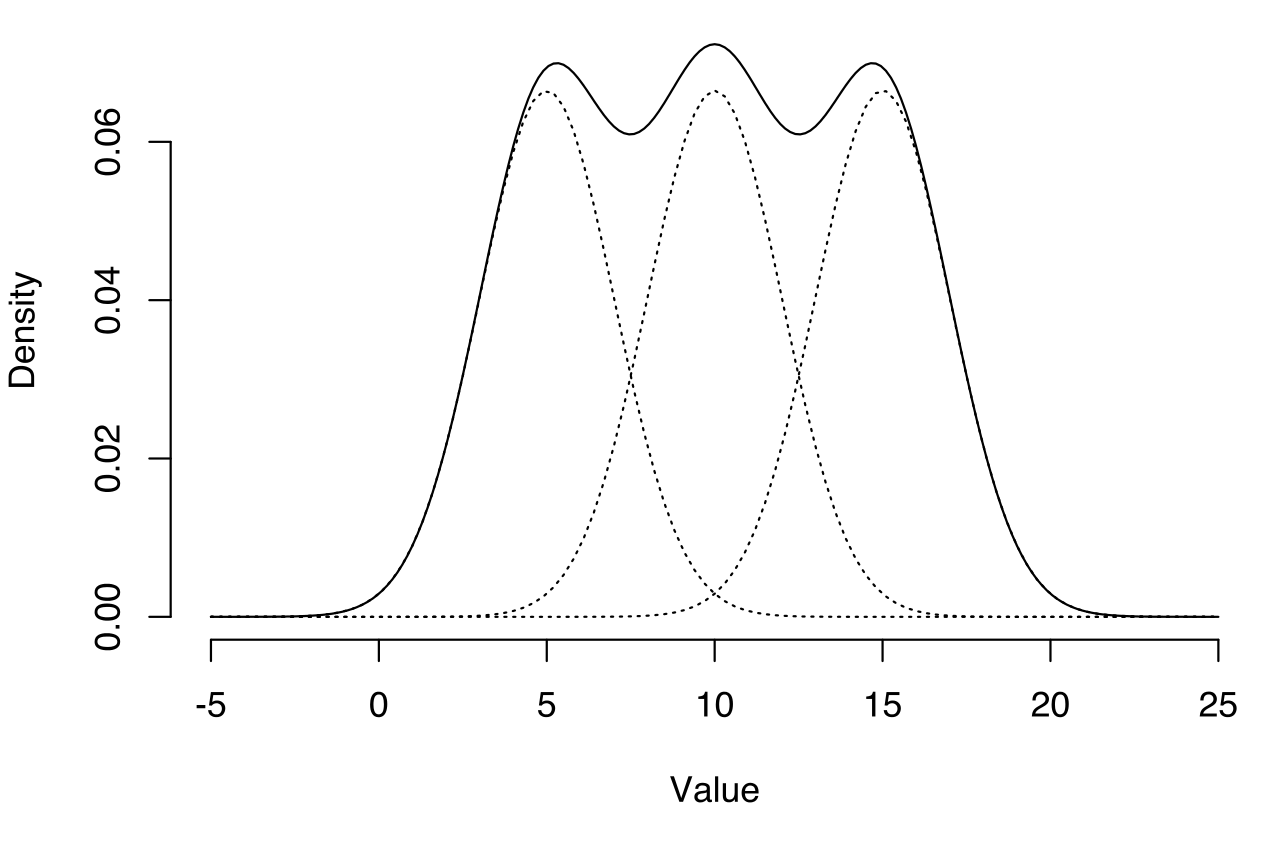
\includegraphics[width=0.6\textwidth]{fig/gaussian-mixture-distribution.png}
    \caption{混合分布}
    \label{fig:mix-dist}
\end{figure}

由于对数收益率的的可叠加性(较长时间内的对数收益率可分解为较短时间间隔对数收益率相叠加),并且利用上述正态分布性质,可知正态分布随机变量$d\ln S$(极短时间内)与叠加之后的$\Delta \ln S$(较长时间内)都应服从\textbf{正态分布}。

对比\textbf{比例收益率}在极短时间内(连续形式)与较长时间内(离散形式):
\begin{gather*}
    \frac{dS_t}{S_t} = \mu dt + \sigma dZ_t \\
    \frac{\Delta S_t}{S_t} = \mu \Delta t + \sigma(Z_T - Z_t)
\end{gather*}

单期百分比收益率虽然在极短时间(连续形式)服从正态分布。对于期数为$n$的多期的百分比收益,应有:
\begin{equation*}
    1+R_{0,n} = (1+R_{0,1})(1+R_{1,2})\dots(1+R_{n-1,n})
\end{equation*}

这里可以看到,若假定资产的收益率分布为正态分布,有如下\textbf{缺点}:首先,多期的百分比收益率为单期收益的乘积,因此将不再服从正态分布。且由于分母$S_t$不断改变,并不能通过叠加的形式得到较长时间的分布(对数收益率的优点),即:
\begin{equation*}
    \frac{S_n - S_0}{S_0} \neq \frac{S_1- S_0}{S_0} + \frac{S_2-S_1}{S_1} + \dots + \frac{S_{n}-S_{n-1}}{S_{n-1}}
\end{equation*}

第二,百分比收益率的取值范围为$[-100\%,+\inf)$,而正态分布可以取任何值,并不存在下边界。第三,实证结果发现许多资产收益率数据都具有正的超额峰度,即相比使用样本均值与方差确定的正态分布相比,具有尖峰肥尾的性质。

\section{BSM 偏微分方程(PDE方法)}

\subsection{假设}
\begin{itemize}
    \item 人性假设
    \begin{itemize}[leftmargin=2em]
        \item 不存在无风险套利机会(无套利)
    \end{itemize}
    \item 完美世界
    \begin{itemize}
        \item 允许卖空标的证券
        \item 没有交易费用和税收
        \item 证券交易时连续的,价格变动也是连续的
        \item 所有证券都完全可分
    \end{itemize}
    \item 可交易资产
        \begin{itemize}
            \item 证券价格遵循几何布朗运动,即$\mu$和$\sigma$为常数
            \item 衍生品有效期内,无风险利率r为常数
            \item 衍生证券有效期内,标的证券没有现金收益支付
        \end{itemize}
\end{itemize}

\subsection{推导}

假设股票价格$S_t$遵循几何布朗运动,以及其离散形式有:
\begin{align*}
    d S_t & = \mu S_t dt + \sigma S_t d Z_t \\
    \Delta S_t & = \mu S_t \Delta t + \sigma S_t \Delta Z_t
\end{align*}

假设衍生品价格$f(S_t, t)$为$S_t$以及$t$的函数,根据伊藤引理可得其连续和离散形式有:

\begin{align*}
    df(S_t,t) & = \left(\frac{\partial f}{\partial S} \mu S_t  + \frac{\partial f}{\partial t} + \frac{1}{2}\frac{\partial^2 f}{\partial S^2} \sigma^2 S_t^2 \right)dt + \frac{\partial f}{\partial S} \sigma S_t dZ_t \\
    \Delta f(S_t,t) & = \left(\frac{\partial f}{\partial S} \mu S_t  + \frac{\partial f}{\partial t} + \frac{1}{2}\frac{\partial^2 f}{\partial S^2} \sigma^2 S_t^2 \right) \Delta t + \frac{\partial f}{\partial S} \sigma S_t \Delta Z_t
\end{align*}

由此可见,股票价格与衍生品价格的风险源均来自$\Delta Z_t$,因此可以构建投资组合,由一单位衍生品空头,以及$\partial f/\partial S$单位证券多头构成,进行对冲消除该风险源:
\begin{equation*}
    \Pi_t = -f_t + \frac{\partial f}{\partial S} S_t
\end{equation*}

在$\Delta t$时间内,该投资组合价值的变化$\Delta \Pi_t$来源其标的资产以及衍生品的价格变动,代入$\Delta S_t$与$\Delta f_t$可得:
\begin{align*}
    \Delta \Pi_t & = -\Delta f_t + \frac{\partial f}{\partial S} \Delta S_t \\
    & = -\left[ \left(\frac{\partial f}{\partial S} \mu S_t  + \frac{\partial f}{\partial t} + \frac{1}{2}\frac{\partial^2 f}{\partial S^2} \sigma^2 S_t^2 \right) \Delta t + \frac{\partial f}{\partial S} \sigma S_t \Delta Z_t \right] + \frac{\partial f}{\partial S} \left( \mu S_t \Delta t + \sigma S_t \Delta Z_t \right) \\
    & = -\left( \frac{\partial f}{\partial t} + \frac{1}{2}\frac{\partial^2 f}{\partial S^2} \sigma^2 S_t^2 \right) \Delta t
\end{align*}

由于此时组合消除了风险,因此组合只应获得无风险收益率:
\begin{align*}
    \Delta \Pi_t & = r \Pi_t \Delta t \\
    -\left( \frac{\partial f}{\partial t} + \frac{1}{2}\frac{\partial^2 f}{\partial S^2} \sigma^2 S_t^2 \right) \Delta t & =  r \left( -f_t + \frac{\partial f}{\partial S} S_t \right) \Delta t
\end{align*}

整理等式,消去$\Delta t$,即可得到\textbf{BSM偏微分方程}(Black-Scholes equation)。由于使用了Delta对冲的方法消除了其中的随机性,最终结果中并不包含任何随机过程,为普通的偏微分方程,为非随机微分方程。求解PDE需要给定的边界条件,如对于欧式看涨期权,其边界条件有当时间$t=T$到达其期限,期权价格$C=\max(S(T)-K,0)$。
\begin{equation*}
    \frac{\partial f}{\partial t} + r S_t \frac{\partial f}{\partial S} + \frac{1}{2} \sigma^2 S_t^2 \frac{\partial^2 f}{\partial S^2} = r f_t
\end{equation*}

\section{BSM公式(鞅方法)}

\subsection{风险中性世界}

\textbf{风险中性定价理论}就来源于BSM微分方程中的一个关键性质,在推导的过程中所有变量,如:股票价格、时间、波动率、无风险利率,均都不涉及投资者的风险偏好。在推导BSM微分方程中,使用Delta对冲方法消除了随机源之后。在不存在无风险套利的市场中,投资组合的收益率必须等于无风险收益率,否则就存在套利机会(\textbf{注意}:这一性质来源于无套利,而非假设)。因此最终结果中中并不包含预期收益率$\mu$,因为投资者对于风险的厌恶程度越高,其所要求的$\mu$也就越高。因此我们可以利用这个特点,即风险偏好在方程中不出现,即其可以随意取值,均不会影响方程的解。因此在计算期权价格中,可以使用任意风险偏好,而最简单的就是\textbf{假设所有投资者都是风险中性的}。所有投资的回报率期望均为无风险利率$r$,对风险中性的投资者而言,他们对风险的态度是中性的,因此不需要额外的风险溢酬。在一个风险中性世界里,任何现金流的现值都可以通过对其期望值以无风险利率贴现来得到。因此利用风险中性定价原理对衍生品定价的过程如下:
\begin{itemize}
    \item 假定标的资产的收益率期望为无风险利率(即假定$\mu=r$)
    \item 计算衍生产品到期时收益的期望
    \item 用无风险利率$r$对衍生品收益期望进行贴现。
\end{itemize}

风险中性定价是获得期权定价公式的一个人为工具或数学方法,其求得的解不但在风险中性世界中成立,在现实世界中也成立。当我们从风险中性世界换到风险厌恶世界时,两件事会发生:股票价格变动的增长率期望以及对衍生产品收益所必需使用的贴现率都将会变化,而这两种变化刚好相互抵消。

\subsection{BSM期权定价公式}

在风险中性世界中,看涨期权价值的期望为:
\begin{equation*}
    \rnE_t \left[ \max(S_T-K,0) \right]
\end{equation*}

欧式看涨期权的现值应为其在$T$时刻期望值以无风险利率进行贴现:
\begin{equation*}
    c = e^{-r(T-t)} \rnE_t \left[ \max(S_T-K,0) \right]
\end{equation*}

同时在风险中性世界下,漂移率$\mu$应等于无风险收益率r,因此有:
\begin{equation*}
    \ln S_T - \ln S_t \sim N \left((r-\frac{\sigma^2}{2})(T-t), \sigma^2(T-t)\right)
\end{equation*}

已知:
\begin{equation*}
    S_T = S_t \exp\left[\left(r-\frac{\sigma^2}{2}\right)\left(T-t\right) + \sigma\left(W_T - W_t \right)\right]
\end{equation*}

已知$Y = \frac{W_T - W_t}{\sqrt{T-t}} \sim N(0,1)$服从标准正态分布,其概率密度函数为:
\begin{equation*}
    \varphi(y) = \frac{1}{\sqrt{2\pi}} e^{-\frac{1}{2}y^2}
\end{equation*}

在风险中性下的期望,可以改写为如下积分的形式:
\begin{align*}
    \rnE_t \left[ \max(S_T-K,0) \right] & = \rnE_t \left[ S_t e^{(r-\frac{1}{2}\sigma^2)(T-t) + \sigma\sqrt{T-t}Y} - K \right]^+ \\
    & = \int_{-\infty}^{\infty} \left( S_t e^{(r-\frac{1}{2}\sigma^2)(T-t) + \sigma\sqrt{T-t}y} - K \right)^+ \varphi(y) dy
\end{align*}

当$S_t e^{(r-\frac{1}{2}\sigma^2)(T-t) + \sigma\sqrt{T-t}Y} - K \geq 0$时,有$y \geq \frac{ \ln (K/S_t) - (r-\frac{1}{2}\sigma^2)(T-t)}{\sigma\sqrt{T-t}}$,设其为$-d_2$,同时假设$d_1 = d_2 + \sigma \sqrt{T-t}$。
\begin{align*}
    \rnE_t \left[ \max(S_T-K,0) \right] & = \int_{-\infty}^{\infty} \left( S_t e^{(r-\frac{1}{2}\sigma^2)(T-t) + \sigma\sqrt{T-t}y} - K \right)^+ \varphi(y) dy \\
    & = S_t e^{(r-\frac{1}{2}\sigma^2)(T-t)} \int_{-d_2}^{\infty} e^{\sigma\sqrt{T-t} y} \varphi(y)dy - K\int_{-d_2}^{\infty} \varphi(y)dy \\
    & = S_t e^{(r-\frac{1}{2} \sigma^2) (T-t)} \int_{-d_2}^{\infty}{e^{\sigma\sqrt{T-t}y} \frac{1}{\sqrt{2\pi\ }}e^{-\frac{y^2}{2}}dy} - KN\left(d_2\right) \\
    & = S_t e^{r(T-t)} \int_{-d_2}^{\infty} \frac{1}{\sqrt{2\pi}} e^{\left( -\frac{\sigma^2 (T-t)}{2} + \sigma\sqrt{T-t}y - \frac{y^2}{2} \right)} dy - KN(d_2) \\
    & = S_t e^{r(T-t)} \int_{y = -d_2}^{y = \infty} \frac{1}{\sqrt{2\pi}}e^{-\frac{\left(y-\sigma\sqrt{T-t}\right)^2}{2}}dy - KN(d_2) \\
    &\hspace{4em} \text{(换元法:$u =y -\sigma\sqrt{T-t}$)} \\
    & =S_t e^{r(T-t)} \int_{u = -d_2-\sigma\sqrt{T-t}}^{u = \infty} \frac{1}{\sqrt{2\pi\ }}e^{-\frac{u^2}{2}}du - KN(d_2) \quad \text{($dy = du$)} \\
    & = S_t e^{r(T-t)} \int_{-d_1}^{\infty} \frac{1}{\sqrt{2\pi}}e^{-\frac{u^2}{2}} du - KN(d_2) \\
    & = S_t e^{r(T-t)}N(d_1) - KN(d_2)
\end{align*}

得到\textbf{BSM公式}(Black-Scholes formula),即欧式看涨期权的定价公式,其中$N(\cdot)$为标准正态分布的累积分布函数(CDF)。
\begin{equation*}
    \boxed{
        c = S_t N(d_1) - Ke^{-r(T-t)} N(d_2)
    }
\end{equation*}

此时$d_1$和$d_2$分别为:
\begin{align*}
    d_1 &= \frac{\ln \frac{S_t}{K} + (r+\frac{1}{2}\sigma^2)(T-t)}{\sigma\sqrt{T-t}} \\
    d_2 &= \frac{\ln \frac{S_t}{K} + (r-\frac{1}{2}\sigma^2)(T-t)}{\sigma\sqrt{T-t}}
\end{align*}

并且已知期权平价公式:
\begin{equation*}
    c + K e^{r(T-t)} = p + S_t
\end{equation*}

将BSM看涨期权定价公式代入:
\begin{align*}
    p & = c + K e^{-r(T-t)} - S_t \\
    & = S_t N(d_1) - Ke^{-r(T-t)} N(d_2) +  Ke^{-r(T-t)} - S_t \\
    & = S_t (N(d_1) - 1) - K e^{-r(T-t)}(N(d_2)-1) \\
    & = S_t (-N(-d_1)) - K e^{-r(T-t)}(-N(-d_2)) \\
    & = K e^{-r(T-t)}N(-d_2) - S_t N(-d_1)
\end{align*}

可得欧式看跌期权定价公式,有:
\begin{equation*}
    \boxed{
    p = K e^{-r(T-t)}N(-d_2) - S_t N(-d_1)
    }
\end{equation*}

\subsection{关于\tops{$N(d_1)$}与\tops{$N(d_2)$}}

期权的价值取决于行权后的收益,对于未能行权的期权,其收益为零,价值也为零。对于行权的期权,其收益决定于两个重要的不确定性因素:
\begin{itemize}
    \item 行权概率:期权到期是否能够行权,或是否为实值期权
    \item 行权收益:如果能够行权,那么收益的期望到底能有多少
\end{itemize}

那么$N(d_2)$与$N(d_1)$对应了上述两个不确定性的概率,以欧式看涨期权为例,$N(d_2)$为在\uline{风险中性世界}中,股票被行权的概率,即为$P(S_T>K)$。因此BSM欧式看涨期权第二项,$Ke^{-r(T-t)}N(d_2)$为在当前时刻(折现后),考虑了行权概率后,所需支付的执行价格,为成本。

如果将第二项理解为成本,那么第一项代表着考虑行权概率后,在当前时间点的股票收益期望。要能有收益,先决条件是能行权,即首先应有$S_T>K$。因此股票在行权时的价值应为一个条件期望$\E[S_T | S_T >K]$,是基于在行权价之上。此条件期望在乘以行权概率$N(d_2)$,并折现到当前时点,应为第一项。应有:
\begin{equation*}
    e^{r(T-t)} \E[S_T | S_T >K] N(d_2) = S_t N(d_1)
\end{equation*}

将上式中的$S_t$代换为$e^{r(T-t)}E[S_T]$:
\begin{equation*}
    e^{r(T-t)} \E[S_T | S_T >K] N(d_2) = S_t e^{r(T-t)}\E[S_T] N(d_1)
\end{equation*}

得到:
\begin{equation*}
    N(d_1) = \frac{\E[S_T | S_T >K]}{\E[S_T]} N(d_2)
\end{equation*}

由于最终的股票的收益并不独立于股票价格,这与行权价独立于股票价格不同,因此$N(d_1)$是基于股票价格加权后的行权概率。$N(d_1)$在数学上还有另外的解释,它是“以股票波动率$N(d_1)$为市场风险定价,并在以股票为计价单位时,期权被行权的概率”。

\subsection{使用BSM公式注意事项}

在实际使用过程,与进行计算的过程中有如下\text{注意点}
\begin{itemize}[leftmargin=4em]
    \item 在计算时,期限、漂移率(无风险利率)、波动率的时间单位应匹配(一般以年为单位,使用交易日计算)
    \item 由于只有交易日才有历史数据与收益率数据,波动率使用交易天数进行年化,中国240天左右(240天,每月20天),美国252天,每月21天
    \item 无风险利率选择即期利率(Spot rate)而非到期收益率(YTM,真实收益率,票息5\%,但非平价发行)
    \item 波动率为一个时间窗口内(为年),日频连续复合收益率或对数收益率($\ln\frac{S_{t+1}}{S_{t}}$)标准差进行年化得到。
    \item 已实现日频波动率(交易日才有波动率)乘以$\sqrt{252}$(一天的方差为$s^2$,由于方差可加,252个交易日的方差即为$s^2 \times 252$,标准差或波动率为$s\sqrt{252}$)。同理,月频收益率得到的波动率应乘以$\sqrt{252/21}$进行年化。
    \item 如果到期时间(time to maturity)是根据日历日(calendar day)计算,那么此时的隐含波动率则为每日历日(per calendar day),如VIX计算是根据365日历日年化
    \item BS隐含波动率的如上所述,即为年化波动率
\end{itemize}

\subsection{期权价格合理边界}

对于期权价格,有上下边界如下,注意不是BSM偏微分方程中的边界条件:
\begin{itemize}
    \item 由于期权只有权利没有义务,因此无论欧式期权或美式期权,其价格应为正,即$C>0$与$P>0$
    \item 看涨期权的上边界应为其标的资产价格,即$C_t \leq S_t$,由于看涨期权给予购买标的资产的权利,因此其价值不应超过标的资产价格
    \item 看跌期权的上边界为行权价折现,即$P_t \leq e^{-r(T-t)}K$,与看涨期权最大值同理,看跌期权给予以行权价$K$卖出标的资产的权利,且股票价格最低为0,因此其价值不应超过行权价的现值
    \item 对于期权的下边界,则应有应大于其内在价值。对于有红利资产,则应扣除其红利,再计算其内在价值
    \item 对于完美市场,应有看涨期权下边界为$C_t \geq \max \left[ S_t-Ke^{-r(T-t)} , 0 \right]$
    \item 同理,在完美市场中,看跌期权下边界为$P_t \geq \max \left[ Ke^{-r(T-t)} - S_t,0 \right]$
    \item 假设标的资产的红利率(Dividend yield)为$q$,那么应将将股票价格$S$替换为$S e^{-q(T-t)}$
\end{itemize}

因此对于看涨期权,其边界应有:
\begin{equation*}
    \max\left[ S_t - Ke^{-r(T-t)},0 \right] \leq C_t \leq S_t 
    \quad \text{或} \quad
    \max\left[ (F_t - K) B_t,0 \right] \leq C_t \leq F_t B_t
\end{equation*}

同理对于看跌期权,其边界应用:
\begin{equation*}
    \max\left[ Ke^{-r(T-t)} - S_t,0 \right] \leq P_t \leq K e^{-r(T-t)}
    \quad \text{或} \quad
    \max\left[ (K - F_t) B_t,0 \right] \leq P_t \leq K B_t
\end{equation*}

\subsection{Black公式与分红}

对于Black公式:
\begin{align*}
    C &= e^{-r\tau}\left[FN(d_1) - KN(d_2)\right] \\
    P &= e^{-r\tau}\left[KN(-d_2) - FN(-d_1)\right]
\end{align*}

其中有:
\begin{align*}
    d_1 &= \frac{\ln(F/K) + \frac{1}{2} \sigma^2 \tau}{\sigma \sqrt{\tau}} \\
    d_2 &= \frac{\ln(F/K) - \frac{1}{2} \sigma^2 \tau}{\sigma \sqrt{\tau}}
    = d_1 - \sigma \sqrt{\tau}
\end{align*}

假设分红的现值为PVD为未来一系列分红的贴现,即$\text{PVD} = \sum_{i=1}^{n} D_{t_i} e^{r_{t_i} t_i}$,$D_{t_i}$为在未来$t_i$时刻的分红,$r_{t_i}$为在未来$t_i$时刻的贴现率。那么应有关系$e^{-r\tau}F = S-\text{PVD}$,将其代入上述Black公式中,可得考虑了分红现值的Black公式:
\begin{align*}
    C &= \left(S-\text{PVD}\right) N(d_1) - e^{-r\tau} KN(d_2) \\
    P &= e^{-r\tau}KN(-d_2) - \left(S-\text{PVD}\right) N(-d_1)
\end{align*}

此时:
\begin{align*}
    d_1 &= \frac{\ln\left[\left( S-\text{PVD} \right) e^{-r\tau} /K\right] + \frac{1}{2} \sigma^2 \tau}{\sigma \sqrt{\tau}} \\
    d_2 &= d_1 - \sigma \sqrt{\tau}
\end{align*}

\section{希腊值}

BSM定价公式的核心价值在于它构建了量化数学模型,以此可以计算期权的各种风险敞口,这对于将期权交易者至关重要。由BSM公式出发可以方便的求出期权价格对标的资产、时间、利率、波动率的偏导数,从而确定期权在这些因素上的风险敞口,常见的风险敞口由五类,由希腊字母表示,称为\text{希腊值},分别是:Delta、Gamma、Vega、Theta与Rho。

\subsection{正态分布与性质}

对于正态分布或高斯分布(Gaussian distribution),其\textbf{概率密度函数}(Probability Density Function,PDF):
\begin{equation*}
    f(x;\mu,\sigma) = \frac{1}{\sigma\sqrt{2\pi}} e^{-\frac{1}{2}\left(\frac{x-\mu}{\sigma} \right)^2}
\end{equation*}

则有$N(x)$为标准正态分布(Standard normal distribution)的\textbf{累积分布函数}(CDF,Cumulative Distribution Function)为:
\begin{equation*}
    N(x) = \frac{1}{\sqrt{2\pi}} \int_{-\infty}^{x}e^{-\frac{z^2}{2}}dz
\end{equation*}

则有$N'(x)$为标准正态分布的概率密度函数:
\begin{equation*}
    N'(x) = \frac{1}{\sqrt{2\pi}} e^{-\frac{x^2}{2}}
\end{equation*}

由于正态分布的对称性,易知有如下性质:
\begin{equation*}
    N(-x) = 1-N(x) \qquad \qquad
    N'(x) = N'(-x)
\end{equation*}

\subsection{希腊值定义与理解}

期权是可以高度量化的工具,为了衡量单一因素对期权价格变化的影响,在数学中即为求导。因此令期权价格价格为V:
\begin{itemize}
    \item $\text{Delta} = \dfrac{\partial V}{\partial S}$:对标的价格的一阶导
    \item $\text{Gamma}  = \frac{\partial^2 V}{\partial S^2}$:对标的价格的二阶导
    \item $\text{Vega} = \frac{\partial V}{\partial\sigma}$:对波动率的一阶导
    \item $\text{Theta} = -\frac{\partial V}{\partial \tau}$:对期限的一阶导
    \item $\text{Rho} = \frac{\partial V}{\partial r}$:对无风险利率的一阶导
\end{itemize}

\subsubsection{多空对希腊字母的影响}

对于Delta,很容易记忆,看涨期权多头受益于标的资产上涨,符号为正,空头相反,符号为负。而看跌期权多头,由于标的资产价格上涨亏损,符号为负,空头相反,符号为正。对于期权多头(看涨或看跌)其Gamma或Vega都为正,都不断的损失时间价值,Theta为负,空方则相反。期权多方的曲线为下凸,因Gamma的存在使得期权多头“赚得多,亏得少”,符号为正。而期权空方的曲线为上凸,由于Gamma存在使得其“赚得少,亏得快”,符号为负。对于期权多头(持有),波动率上升,使得期权价格上涨,因此Vega为正。
\begin{table}[H]
\centering
\begin{tabular}{@{}cccccc@{}} \toprule
           & Delta & Gamma & Vega & Theta & Rho \\ \midrule
Long Call  & $+$ & $+$ & $+$ & $-$ & $+$ \\
Long Put   & $-$ & $+$ & $+$ & $-$ & $-$ \\
Short Call & $-$ & $-$ & $-$ & $+$ & $+$ \\
Short Put  & $+$ & $-$ & $-$ & $+$ & $+$ \\ \bottomrule
\end{tabular}
\end{table}

\subsubsection{Delta}

如下图所示看涨期权的Delta值在$(0,1)$之间,看跌期权的Delta值在$(-1,0)$之间。对于BSM而言,看涨期权Delta与看跌期权Delta有如下关系$\text{Delta}_C - \text{Delta}_P = 1$。期权价格与标的资产价格的关系如下:
\begin{figure}[H]
    \centering
    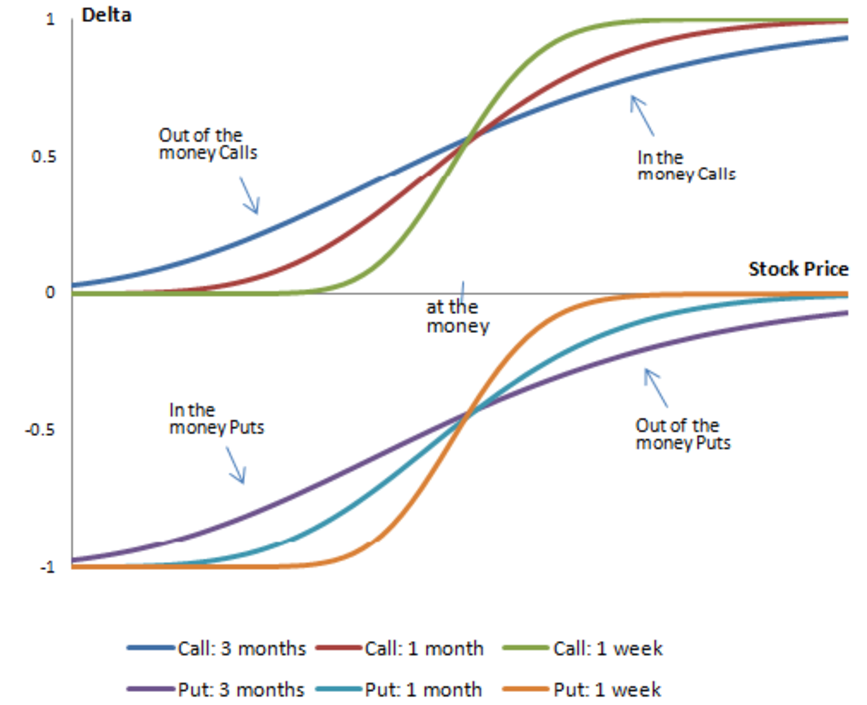
\includegraphics[width=0.68\textwidth]{fig/delta-stock.png}
    \caption{Delta与标的资产价格之间的关系}
    \label{fig:delta-stock}
\end{figure}

如上图\ref{fig:delta-stock}所示,对于期权权利方(多方),无论看涨看跌期权,随着标的价格上涨,Delta也增大。反之若为期权义务方(空方),则随着标的价格的下跌,Delta也减小。并且可以看到当Delta的\uline{绝对值}约在$0.25$附近时,看涨看跌期权都为虚值期权(OTM)。当期权处于虚值状态时,标的资产价格的变动对期权价格的影响较小。当Delta的\uline{绝对值}约$0.5$附近时,看涨与看跌期权均为平值期权(ATM),可以看到此时斜率最大,即Gamma最大(Delta对S求导)。当Delta的\uline{绝对值}约$0.75$附近时,看涨与看跌期权均为实值期权(ITM),此时标的资产变动与期权价值变动接近于$1:1$。

可以将Delta理解为期权价格与标的价格的贴合程度,以看涨期权为例,当为深度实值时,贴合程度最好,标的价格变化1单位,期权价格变化1单位。即实值贴合好,对股价变动敏感,相反虚值贴合差,对股价变动不敏感。如下图所示,随着期限不断衰减,期权价格曲线将越来越贴合期权内在价值。并且不同在值程度期权的Delta,也将随着期限的衰减,差异不断加大。实值期权Delta将加速趋近1,而虚值期权将加速趋近0,平值期权变化较小。
\begin{figure}[H]
    \centering
    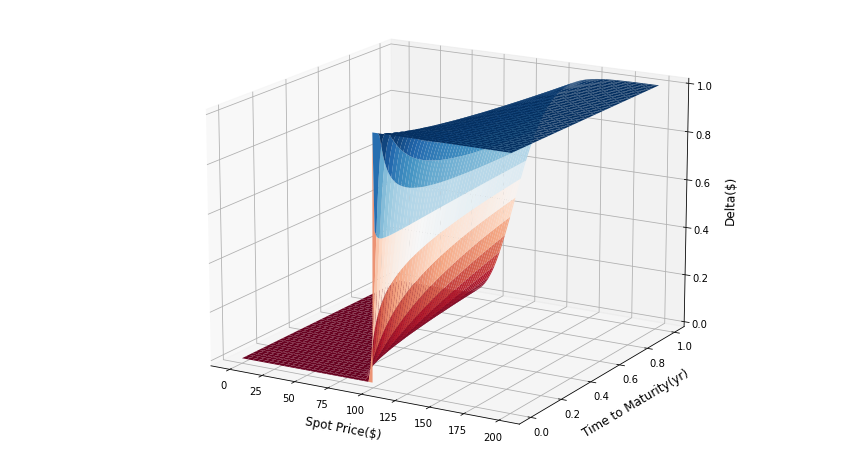
\includegraphics[width=\textwidth]{fig/delta-call-surf.png}
    \caption{看涨期权多方Delta}
    \label{fig:delta-call-surf}
\end{figure}

\begin{figure}[H]
    \centering
    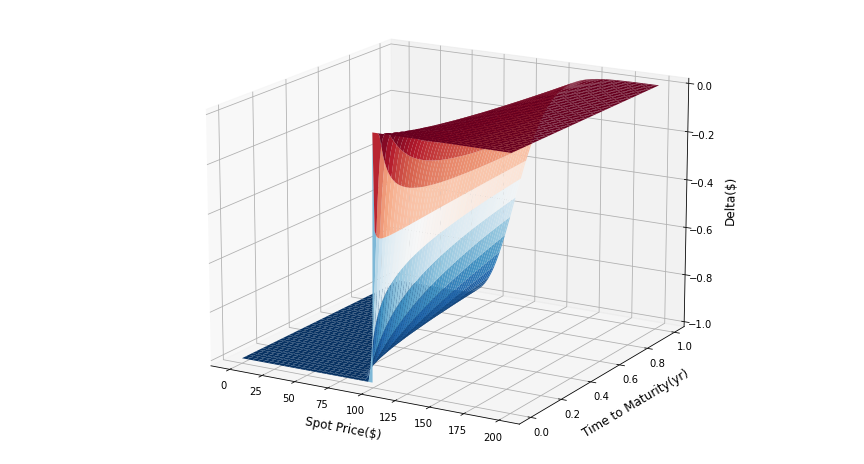
\includegraphics[width=\textwidth]{fig/delta-put-surf.png}
    \caption{看跌期权多方Delta}
    \label{fig:delta-put-surf}
\end{figure}

\subsubsection{Gamma}

若以期权价格为纵轴,标的资产价格为横轴,得到期权收益,如图\ref{fig:call-vs-stock}。那么Delta为该曲线切线的斜率,为一阶导,衡量期权价格对标的资产变动的敏感程度。Gamma为该曲线的二阶导,为Delta的变化速度,或曲线弯曲程度或加速度,衡量Delta对标的资产价格变动的敏感程度。同时Gamma如图\ref{fig:delta-stock}中所示,为Delta与标的资产价格关系的一阶导:
\begin{equation*}
    \Gamma = \frac{\partial \Delta}{\partial S} = \frac{\partial^2 V}{\partial S^2}
\end{equation*}

期权权利方(多方),有正的Gamma,标的资产价格的变化对投资者有利。具体而言,当价格上涨的时候,此时对投资者有利,随着标的资产价格的不断上涨,期权所带来的盈利越多。相反当价格下跌时,此时对投资者不利,但随着标的资产的不断下跌,损失越来越小。而作为做市商等,卖期权(期权空方),则有负的Gamma。此时与期权投资者相反,价格上涨时,盈利减慢,而价格下跌时,损失增大。正Gamma为凸函数(Convex,下凸),负Gamma为凹函数(Concave,上凸),另外可以看到在平值点的Gamma最大,看涨期权与看跌期权的Gamma相同。
\begin{figure}[H]
    \centering
    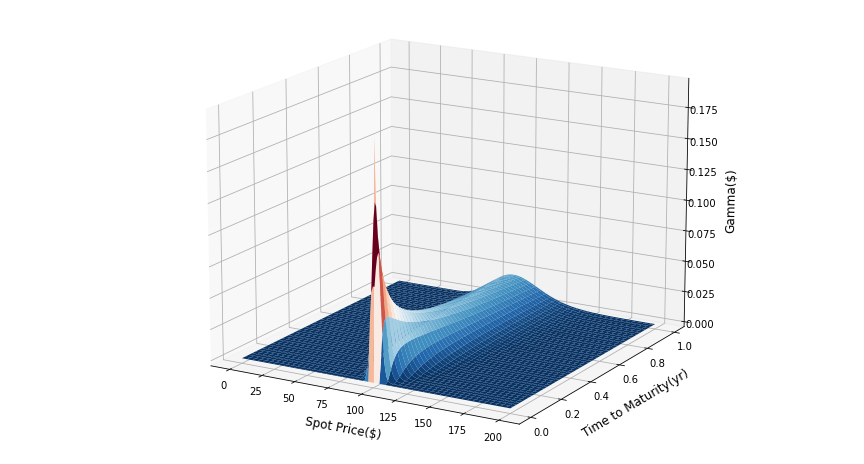
\includegraphics[width=\textwidth]{fig/gamma-surf.png}
    \caption{看涨看跌期权多方Gamma}
    \label{fig:gamma-surf}
\end{figure}

另外需要注意,\uline{只有期权有Gamma值},因此为了达到投资组合$\Pi$的Gamma中性状态,只能通过期权头寸的调整获得。实现Gamma中性往往会带来Delta的非中性,还需要调整标的资产或者期货头寸才能使得投资组合同时达到Delta中性与Gamma中性。

\subsubsection{Vega}

Vega体现的为期权价格对波动率的敏感程度,即波动率变化$1\%$对期权价格的影响。对于期权的多头,其Vega为正,意味着隐含波动率的正向变化对其有利,空头则相反。看涨期权与看跌期权的Vega相同。当调整期权头寸使投资组合为Vega中性时,Gamma也会随之改变,因此要达到Vega与Gamma同时中性,需要使用同一标的的两种期权。
\begin{figure}[H]
    \centering
    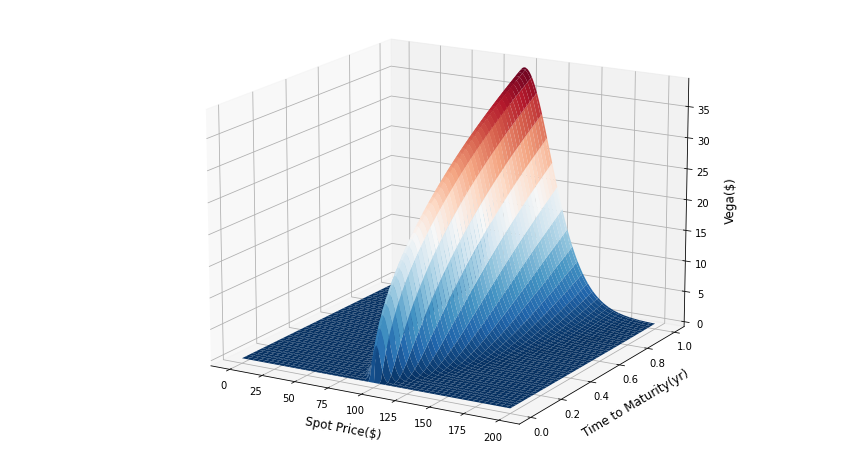
\includegraphics[width=\textwidth]{fig/vega-surf.png}
    \caption{看涨看跌期权多方Vega}
    \label{fig:vega-surf}
\end{figure}

\subsubsection{Theta}

下图期权的时间价值曲线中,随着剩余期限的减小,期权的时间价值在加速衰减。
\begin{figure}[H]
    \centering
    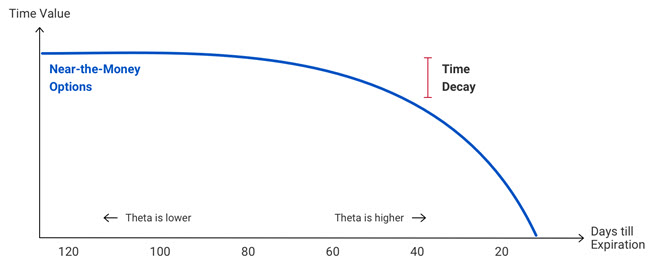
\includegraphics[width=0.8\textwidth]{fig/time-value.jpeg}
    \caption{期权多方时间价值的}
    \label{fig:time-value}
\end{figure}

因此对于期权的多方,其时间价值在不断衰减,有Theta为负。相反,空方则Theta为正。注意:对于Thtea多空符号相同,但值不同。
\begin{figure}[H]
    \centering
    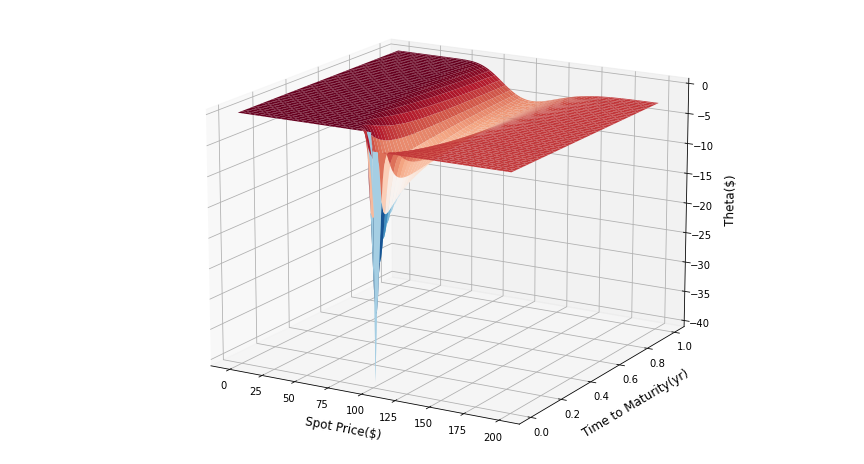
\includegraphics[width=\textwidth]{fig/theta-call-surf.png}
    \caption{看涨期权多方Theta}
    \label{fig:theta-call-surf}
\end{figure}

只有具有高红利的欧式认购期权,Theta也可能为正。另外,可以看到在下图看跌期权多方的Theta中,深度实值的看跌期权,拥有正的Theta(深红色部分)。
\begin{figure}[H]
    \centering
    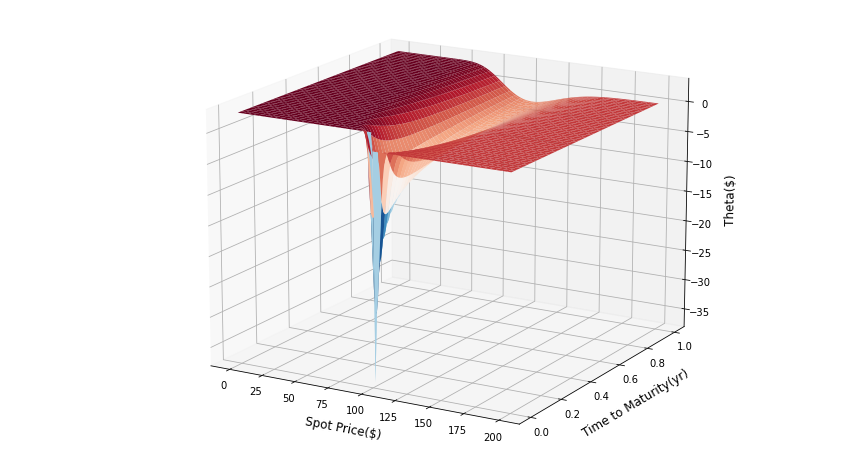
\includegraphics[width=\textwidth]{fig/theta-put-surf.png}
    \caption{看跌期权多方Theta}
    \label{fig:theta-put-surf}
\end{figure}

\subsection{Delta对冲}

Delta为衍生品价格变动与其标的资产价格变动的比率。如果假定股票价格(X)与期权价格(Y)为折线,则其斜率应为Delta,即对股票价格变动一单位,期权价格变动$\Delta$单位。而现实中并非折线,Delta则为两者切线斜率。
\begin{equation*}
    \text{Delta} = \frac{\partial V}{\partial S}
\end{equation*}

而从持有标的资产和衍生品数量分别为$N_S$和$N_V$而言,为了维持对冲结果,易知对于每一单位标的资产,应使用Delta单位衍生品进行对冲。
\begin{equation*}
    \Delta V \times N_V = \Delta S \times N_S \qquad \Rightarrow \qquad
    \text{Delta} = \frac{\partial V}{\partial S} = \frac{N_S}{N_V}
\end{equation*}

而对于投资组合而言,其净Delta(Net portfolio delta)应为组合内所有某合约Delta与该合约数量乘积之和:
\begin{equation*}
    \sum_{i=1}^{n} \text{Delta}_i \times \text{期权合约数}_i
\end{equation*}

同样对于Vega而言,投资组合净Vega(Net portfolio vega)为:
\begin{equation*}
    \sum_{i=1}^{n} \text{Vega}_i \times \text{期权合约数}_i
\end{equation*}

假定股票价格遵循几何布朗运动,则有在现实测度(Physical probability measure)下:
\begin{equation*}
    \frac{dS_t}{S_t} = \mu dt + \sigma dW_t
\end{equation*}

根据伊藤引理:
\begin{equation*}
    f(T,W_T) =f(t,W_t) = \int^T_t \frac{\partial f}{\partial u}du + \int^T_t \frac{\partial f}{\partial S} dW_t \frac{1}{2} + \int^T_t\frac{\partial ^2 f}{\partial S^2} 
\end{equation*}

【待整理】 在Bakshi and Kapadia 2003中,

在一段时间内的使用看涨看跌期权进行Delta对冲(\textbf{注意:}由几何布朗运动与伊藤过程推到而来,因此看涨看跌期权形式相同,买入看涨看跌期权,并卖出股票,净投资金额获得无风险收益)。
\begin{equation*}
    \text{Call Gain} = C_{t+\tau} - C_t - \Delta_t ( S_{t+\tau}-S_t) - \frac{r\tau}{365}(C_{t+\tau} - \Delta_t S_t)
\end{equation*}
\begin{equation*}
    \text{Put Gain} = P_{t+\tau} - P_t - \Delta_t ( S_{t+\tau}-S_t) - \frac{r\tau}{365}(P_{t+\tau} - \Delta_t S_t)
\end{equation*}

Long call, short delta stock/ short call, long delta stock

Long put, long delta stock/ short put, short delta stock

此时需要注意,Put的Delta为负

假设持有时间为t到t+1,具体操作为在t时刻时,买入Delta份看涨看跌期权(消耗现金$-C_{t}$),卖出一份股票(获得现金$+ \Delta S_{t}$)。而在t+1时刻进行平仓,那么需要卖出Delta份看涨看跌期权(获得现金$C_{t+1}$),买入一份股票(消耗现金$- \Delta S_{t+1}$)。因此整体投资组合的收益应为:
\begin{equation*}
    ( C_{t+1} -\Delta S_{t+1} ) + ( -C_{t} + \Delta S_{t} ) =  (C_{t+1} - C_{t}) - \Delta (S_{t+1} - S_{t})
\end{equation*}

\subsection{希腊值分解}

\subsubsection{泰勒级数}

级数为无穷的序列(sequences)(或无穷多项)的和。泰勒级数(Taylor series)使用无限项序列来表示一个函数,每项由该函数在某一点的导数求得。一个函数的有限项的泰勒级数叫做泰勒多项式(Taylor polynomial)。对于一元函数在$x=a$处展开的泰勒级数有:
\begin{align*}
    f(x) &= \sum^{\infty}_{n=0} \frac{f^{(n)}(a)}{n!}(x-a)^n \\
    &= \frac{f(a)}{1}(1)+ \frac{f'(a)}{1}(x-a) + \frac{f''(a)}{2}(x-a)^2 + \frac{f'''(a)}{6}(x-a)^3 + \dots \\
    &= f(a) + f'(a)(x-a) + \frac{f''(a)}{2}(x-a) + \frac{f'''(a)}{6}(x-a)^3 + \dots
\end{align*}

\begin{example}
    当$f(x) = \ln(x)$时候:
    \begin{equation*}
        \ln(x) = \ln(a) + \frac{1}{a}(x-a) - \frac{1}{2a^2}(x-a)^2 + \frac{1}{3a^3}(x-a)^3 - \frac{1}{4a^4}(x-a)^4 + \dots
    \end{equation*}

    整理可知,对数变化与百分比变化:有如下近似关系:
    \begin{equation*}
        \ln\left(\frac{x}{a}\right) = \frac{x-a}{a} + \left( - \frac{1}{2a^2}(x-a)^2 + \frac{1}{3a^3}(x-a)^3 - \frac{1}{4a^4}(x-a)^4 + \dots \right)
    \end{equation*}

    即:
    \begin{equation*}
        \ln x_2 - \ln x_1 = \ln\left(\frac{x_2}{x_1}\right) \approx \frac{x_2-x_1}{x_1}
    \end{equation*}
\end{example}

对于多元函数在$(a,b)$处展开的泰勒级数为:
\begin{align*}
    f(x,y) &= f(a,b) + f'_x(a,b)(x-a) + f'_y(a,b)(y-b) \\
    &\quad + \frac{1}{2}f''_{xx}(a,b)(x-a)^2 + \frac{1}{2}f''_{yy}(a,b)(y-b)^2 +\cancel{2*\frac{1}{2}}f''_{xy}(a,b)(x-a)(y-b)
\end{align*}

\subsubsection*{原理}
假设使用多项式$P(x) = c_0 + c_1 (x-a) + c_2 (x-a)^2 + \dots$近似原函数。则应有多项式与原函数,从零阶导开始至$n$阶导,在$x=a$点的取值都与原函数相同(即从单个点,提取原函数所有导数信息):
\begin{itemize}
    \item $x-a$使得带入a进行计算时,除了当前导数对应次数的项之外都等于零。如原函数在$a$点的二阶导$f''(a)$,对应泰勒级数$x$二次项的系数$c_2$:一阶导为$P'(x) = c_1 + 2c_2(x-a)+\dots$,二阶导为$P''(x) = 2c_2 + 3c_3(x-a)^2 + \dots$,则有$P''(a) = 2c_2 = f''(a)$,此时$c_2 = \tfrac{f''(a)}{2}$
    \item 小于当前求导次数的泰勒级数项,由于求导都为零(如上所示求二阶导后,常数项与一次项都为0),使得多项式每一项的系数$c_n$都独立对应原函数n阶导数值
    \item 系数为$\frac{1}{n!}$是为了取消多次求导的影响,如$P'''(x)=3 \cdot 2 \cdot 1 \cdot c_3(x-a) + \cdots$
\end{itemize}

\subsubsection{基于\tops{$S$}与\tops{$t$}的希腊值分解}

假设投资组合$\Pi$(或期权价格V),为标的资产价格$S$与时间$t$的函数,则有在$(S_0,t_0)$使用泰勒级数展开为:
\begin{align*}
    \Pi(S,T) &= \Pi(S_0,t_0) + \frac{\partial \Pi}{\partial S}(S-S_0) + \frac{\partial \Pi}{\partial t}(t-t_0) \\
    &\quad + \frac{1}{2}\frac{\partial^2 \Pi}{\partial S^2}(S-S_0)^2 + \frac{1}{2}\frac{\partial^2 \Pi}{\partial t^2}(t-t_0)^2 + \frac{\partial^2 \Pi}{\partial S \partial t}(S-S_0)(t-t_0) + \dots
\end{align*}

整理可得(注意:$\Delta$代表变化,并非希腊值):
\begin{equation*}
    \Delta \Pi = \frac{\partial \Pi}{\partial S}\Delta S + \frac{\partial \Pi}{\partial t}\Delta t + \frac{1}{2}\frac{\partial^2 \Pi}{\partial S^2}(\Delta S)^2 + \frac{1}{2}\frac{\partial^2 \Pi}{\partial t^2}\Delta t^2 + \frac{\partial^2 \Pi}{\partial S \partial t}\Delta S \Delta t + \dots
\end{equation*}

将阶数高于$\Delta t$的项忽略(前三项之后):
\begin{equation*}
    \Delta \Pi = \frac{\partial \Pi}{\partial S}\Delta S + \frac{\partial \Pi}{\partial t}\Delta t + \frac{1}{2}\frac{\partial^2 \Pi}{\partial S^2}(\Delta S)^2
\end{equation*}

得到:
\begin{equation*}
    \boxed{
        \Delta \Pi = \Delta S \times \text{Delta} + \Delta t \times \text{Theta} + \frac{1}{2} (\Delta S)^2 \times \text{Gamma}
    }
\end{equation*}

若忽略Theta的影响,只考虑Delta与Gamma。可以发现投资组合的变化可以主要分解为斜率部分与曲度部分。斜率部分由Delta解释,曲度部分由Gamma解释:
\begin{equation*}
    \Delta \Pi \approx \Delta S \times \text{Delta} + \frac{1}{2} (\Delta S)^2 \times \text{Gamma}
\end{equation*}

\begin{figure}[H]
    \centering
    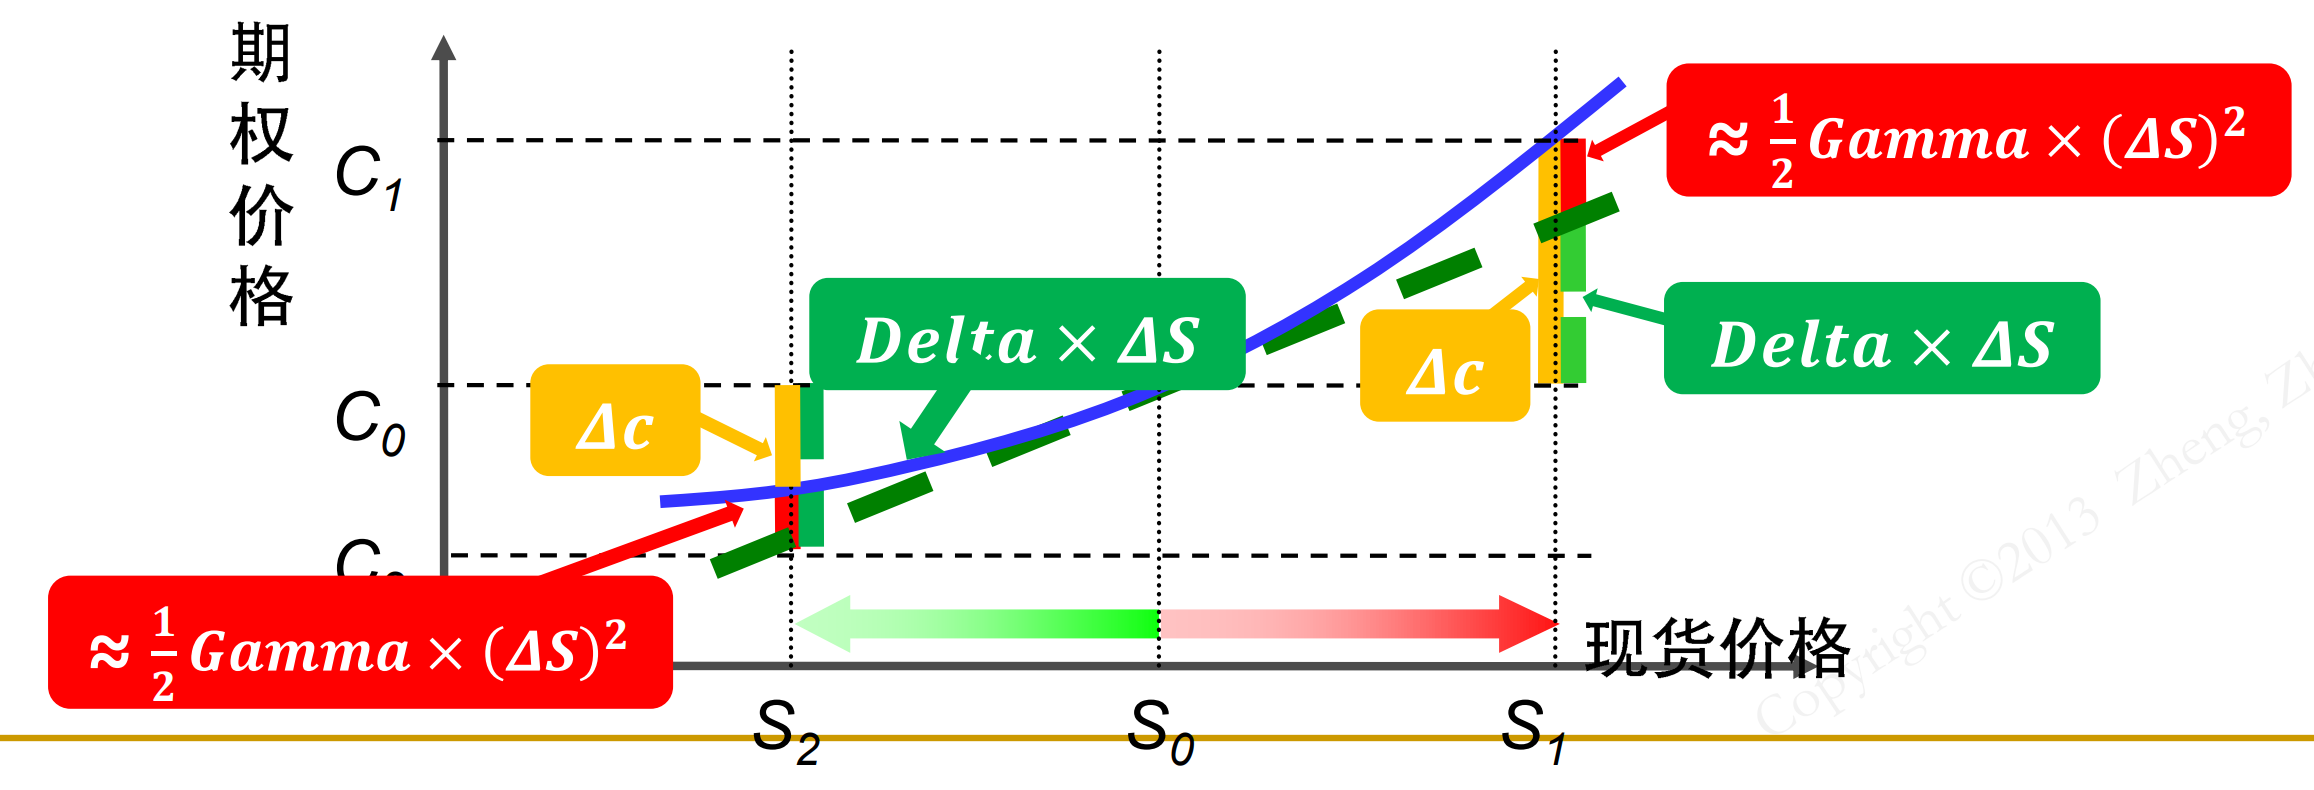
\includegraphics[width=0.8\textwidth]{fig/delta-gamma-decom.png}
    \caption{Delta与Gamma分解}
    \label{fig:delta-gamma-decom}
\end{figure}

由上图可以看到,由于$(\Delta S)^2$为大于等于零,且作为期权多方Gamma为正,因此Gamma项为正。因此可以清楚在图上看到,Gamma对于期权多方的优势,即当标的资产价格上涨时,由于曲度存在,使得在Delta部分收益的基础上,还增加了Gamma部分的收益。而当标的资产下跌时,期权价格虽然损失了与上涨等量的Delta部分的收益,但依然获得了Gamma的收益。这样使得期权多方,赚得多,陪得少。相反,对于期权的空方,或一般为做市商,同理无论标的资产上涨或下跌,都必须损失Gamma部分的收益。使得空方,赚得少,陪得多。

另外可以发现对于一个Delta中立的投资组合,即当$\text{Delta}=0$时,即值只考虑Theta与Gamma时,应有\footnote{见OFOD第十版附录19A\label{ofod_19a}}:
\begin{equation*}
    \Delta \Pi = \Delta t \times \text{Theta} + \frac{1}{2} (\Delta S)^2 \times \text{Gamma}
\end{equation*}

\subsubsection{基于\tops{$S$}与\tops{$\sigma$}的希腊值分解}

在实践中,波动率并非为常数。在短时间内忽略无风险利率的变化,仅仅关注标的资产价格$S$以及隐含波动率$\sigma_{imp}$的变化,作为投资组合$\Pi$(或期权价格V)的变化近似,使用泰勒级数展开,则有\footref{ofod_19a}:
\begin{align*}
    \Delta \Pi &= \frac{\partial \Pi}{\partial S}\Delta S + \frac{\partial \Pi}{\partial \sigma_{imp}}\Delta \sigma_{imp} \\
    &\quad + \frac{1}{2} \frac{\partial^2 \Pi}{\partial S^2}(\Delta S)^2 + \frac{\partial^2 \Pi}{\partial S \partial \sigma_{imp}}\Delta S \Delta \sigma_{imp} + \frac{1}{2} \frac{\partial^2 \Pi}{\partial \sigma^2_{imp}} (\Delta \sigma_{imp})^2 + \dots \\
    &= \Delta S \times \text{Delta} + \Delta \sigma_{imp} \times \text{Vega} \\
    &\quad + \frac{1}{2} (\Delta S)^2 \times \text{Gamma} + \Delta S \Delta \sigma_{imp} \times \text{Vanna} + \frac{1}{2} (\Delta \sigma_{imp})^2 \times \text{Vomma} + \dots
\end{align*}

Delta、Vega、Gamma对应了上式中的前三项,而交易员将$\tfrac{\partial^2 \Pi}{\partial S\partial \sigma_{imp}}$称为Vanna,或理解为Delta的Vega,即对于$\sigma_{imp}$的变动,Delta的敏感程度。将$\tfrac{\partial^2 \Pi}{\partial \sigma^2_{imp}}$称为Vomma,即Vega对于$\sigma_{imp}$的敏感程度,或Vega的Vega。

\subsubsection{BSM分解}

由BSM偏微分方程可知:
\begin{equation*}
    r \Pi = r S_t \frac{\partial \Pi}{\partial S} + \frac{\partial \Pi}{\partial t} + \frac{1}{2} \sigma^2 S^2 \frac{\partial^2 \Pi}{\partial S^2}
\end{equation*}

改写为希腊值的形式:
\begin{equation*}
    \boxed{
        r \Pi = r S_t \times \text{Delta} + \text{Theta} + \frac{1}{2} \sigma^2 S^2 \times \text{Gamma}
    }
\end{equation*}

由上式可见,当一个投资组合即Delta中性又Gamma中性时,有$\text{Theta} = r\Pi$,即投资组合的价值将随时间以无风险连续复利率的速度增长。若假设无风险利率为0,则可得到Theta与Gamma的关系式:
\begin{equation*}
    \text{Theta} + \frac{1}{2} \sigma^2 S^2 \times \text{Gamma} = 0
\end{equation*}

那么可以看到$Theta$与$Gamma$的相互制约关系。对于期权的多头,其Gamma为正,但同时Theta为负。对于空头则相反,有Gamma为负,Theta为正。

\subsection{Black模型的希腊值推导}

对于Black期权模型,其公允价值(Fair value)应有:
\begin{align*}
    C &= e^{-r\tau}\left[FN(d_1) - KN(d_2)\right] \\
    P &= e^{-r\tau}\left[KN(-d_2) - FN(-d_1)\right]
\end{align*}

其中有:
\begin{align*}
    d_1 &= \frac{\ln(F/K) + \frac{1}{2} \sigma^2 \tau}{\sigma \sqrt{\tau}} \\
    d_2 &= \frac{\ln(F/K) - \frac{1}{2} \sigma^2 \tau}{\sigma \sqrt{\tau}}
    = d_1 - \sigma \sqrt{\tau}
\end{align*}

其中有:
\begin{equation*}
    \frac{\partial d_1}{\partial F} = \frac{\partial d_2}{\partial F} = \frac{\frac{\partial \ln(F/K)}{\partial F} \sigma \sqrt{\tau}}{(\sigma \sqrt{\tau})^2} = \frac{\partial (\ln F - \ln K)/\partial F}{\sigma\sqrt{\tau}} = \frac{1}{F\sigma\sqrt{\tau}}
\end{equation*}

\begin{lemma}
    \begin{equation*}
        F N'(d_1) = K N'(d_2)
    \end{equation*}
\end{lemma}

\begin{proof}
    \begin{align*}
        FN'(d_1) &= \frac{F}{\sqrt{2\pi}}e^{-d_1^2/2} \\
        KN'(d_2) &= \frac{K}{\sqrt{2\pi}}e^{-d_2^2/2} = \frac{K}{\sqrt{2\pi}}e^{-d_1^2/2+d_1\sigma\sqrt{\tau}-\sigma^2\tau/2} \\
        &= \frac{K}{\sqrt{2\pi}}e^{-d_1^2/2+\ln(F/K)} 
        \qquad \left(d_1\sigma\sqrt{\tau} = \ln(F/K)+\sigma^2\tau\right) \\
        &= \frac{F}{\sqrt{2\pi}}e^{-d_1^2/2} = FN'(d_1)
    \end{align*}
\end{proof}

\subsubsection{Delta}

可以看到对于Black公式而言,有$\text{Delta}_C - \text{Delta}_P = e^{-r\tau}$:
\begin{align*}
    \text{Delta}_C &= e^{-r\tau}\left[N(d_1) + FN'(d_1)\frac{\partial d_1}{\partial F} - KN'(d_2)\frac{\partial d_2}{\partial F}\right] \\
    &= e^{-r\tau}N(d_1) \\
    \text{Delta}_P &= e^{-r\tau}\left[KN'(-d_2)\frac{\partial d_2}{\partial F} - N(-d_1) - FN'(-d_1)\frac{\partial d_1}{\partial F}\right] \\
    &= e^{-r\tau}\left[ -N(-d_1) \right]
    = - e^{-r\tau} N(-d_1) \\
    &= e^{-r\tau}\left[ N(d_1) -1 \right]
\end{align*}

由远期(期货)的PCP公式:
\begin{equation*}
    C = P + \left( F - K \right) e^{-r(T-t)}
\end{equation*}

对期货价格$F$,求导可得:
\begin{align*}
    \frac{\partial C}{\partial F} &= \frac{\partial P}{\partial F} + e^{-r(T-t)} \\
    \text{Delta}_{C} &= \text{Delta}_{P} + e^{-r(T-t)}
\end{align*}

\subsection{BSM模型的希腊值推导}

当红利率为$q$时,有:
\begin{align*}
    C_t &= S_te^{-q\tau}N(d_1) - Ke^{-r\tau}N(d_2) \\
    P_t &= -S_te^{-q\tau}N(-d_1) + Ke^{-r\tau}N(-d_2)
\end{align*}

其中有:
\begin{align*}
    d_1 &= \frac{\ln(S/K) + (r-q+\frac{1}{2} \sigma^2)\tau}{\sigma \sqrt{\tau}} \\
    d_2 &= \frac{\ln(S/K) + (r-q-\frac{1}{2} \sigma^2)\tau}{\sigma \sqrt{\tau}} = d_1 - \sigma \sqrt{\tau}
\end{align*}

\begin{lemma}
    \begin{equation*}
        \frac{\partial d_2}{\partial S} = \frac{\partial d_1}{\partial S} = \frac{\frac{\partial \ln(S/K)}{\partial S} \sigma \sqrt{\tau}}{(\sigma \sqrt{\tau})^2} = \frac{\partial (\ln S - \ln K)/\partial S}{\sigma\sqrt{\tau}} = \frac{1}{S\sigma\sqrt{\tau}}
    \end{equation*}
    \begin{equation*}
        \frac{\partial d_2}{\partial \tau} = \frac{\partial d_1}{\partial \tau} - \frac{1}{2}\frac{\sigma}{\sqrt{\tau}}
    \end{equation*}
    \begin{equation*}
        \frac{\partial d_2}{\partial \sigma} = \frac{\partial d_1}{\partial \tau} - \sqrt{\tau}
    \end{equation*}
    \begin{equation*}
        \frac{\partial d_2}{\partial r} = \frac{\partial d_1}{\partial r}
    \end{equation*}
\end{lemma}

\begin{lemma}
    对于BSM公式,有:
    \begin{equation*}
        S_t N'(d_1) = Ke^{-r\tau} N'(d_2)
    \end{equation*}
\end{lemma}

\begin{proof}
    已知:
    \begin{align*}
        d_2^2-d_1^2 &= (d_2-d_1)(d_2+d_1) \\
        &= (-\sigma\sqrt{\tau})(2d_1-\sigma\sqrt{\tau}) \\
        &= (-\sigma\sqrt{\tau})\left(\frac{2\ln(S_t/K) + 2(r+\sigma^2/2)\tau}{\sigma\sqrt{\tau}} -\sigma\sqrt{\tau}\right) \\
        &= -2\left[\ln\frac{S_t}{K}+r\tau\right]
    \end{align*}

    同时已知$N'(x)=\frac{1}{\sqrt{2\pi}} e^{-\frac{x^2}{2}}$,则有:
    \begin{equation*}
        \ln\left(\frac{N'(d_1)}{N'(d_2)}\right)
        = -\frac{d_1^2}{2} + \frac{d_2^2}{2}
        = \frac{1}{2} (d_2^2-d_1^2)
        = -\left[\ln\frac{S_t}{K} +r\tau\right]
    \end{equation*}

    对等式两边取指数:
    \begin{align*}
        \frac{N'(d_1)}{N'(d_2)} 
        &= \exp\left( -\left[\ln\frac{S_t}{K} +r\tau\right] \right) \\
        &= \exp \left( \ln\frac{K}{S_t}-r\tau \right) \\
        &= \frac{K}{S_t} e^{-r\tau} \\
        S_t N'(d_1) &= Ke^{-r\tau} N'(d_2)
    \end{align*}
\end{proof}

\subsubsection{Delta}

对于无红利,即$q=0$时,Delta($\Delta$),如上所述,此时看涨期权Delta与看跌期权Delta有如下关系$\text{Delta}_C - \text{Delta}_P = 1$:
\begin{align*}
    \text{Delta}_C &= \frac{\partial C}{\partial S}
    = N(d_1) + \frac{1}{S_t\sigma\sqrt{\tau}} \left[ S_t N'(d_1)-Ke^{-r\tau}N'(d_2) \right] = N(d_1) \\
    \text{Delta}_P &= \frac{\partial P}{\partial S}
    = -N(-d_1) + \frac{1}{S_t\sigma\sqrt{\tau}} \left[ S_t N'(d_1)-Ke^{-r\tau}N'(d_2) \right] \\
    &= -N(-d_1) = -\left[ 1- N(d_1) \right] = N(d_1)-1
\end{align*}

也可从看涨看跌平价关系(PCP)中,对等式两侧对S求导得到:
\begin{gather*}
    C_{t,T} = P_{t,T} +  S_t - K e^{-r(T-t)} \\
    \frac{\partial C}{\partial S} = \frac{\partial P}{\partial S} + 1
\end{gather*}

当已知红利率为$q$时,有:
\begin{align*}
    \text{Delta}_C &= -e^{-q\tau} N(d_1) \\
    \text{Delta}_P &= -e^{-q\tau} N(-d_1)
\end{align*}

此时有:
\begin{align*}
    \text{Delta}_C - \text{Delta}_P 
    &= -e^{-q\tau} \left[ N(d_1) + N(-d_1) \right] \\
    &= -e^{-q\tau} \left[ N(d_1) + 1 - N(d_1) \right] \\
    &= -e^{-q\tau}
\end{align*}

\subsubsection{Gamma}

对于Gamma($\Gamma$)而言,看涨与看跌期权Gamma相同:
\begin{equation*}
    \text{Gamma} = \frac{\partial^2 V}{\partial S^2} = \frac{\partial N(d_1)}{\partial S} = N'(d_1)\frac{\partial d_1}{\partial S} = \frac{N'(d_1)}{S\sigma\sqrt{\tau}}
\end{equation*}

\subsubsection{Vega}

对于Vega而言,看涨与看跌期权Vega相同(注意:此时计算出的波动率为每变化1,期权价格变动情况,而在实际交易中,一般以波动率每变化$1\%$,即变化$0.01$):
\begin{equation*}
    \text{Vega} = \frac{\partial V}{\partial \sigma}  = SN'(d_1)\sqrt{\tau}
\end{equation*}

当红利率为$q$时有:
\begin{equation*}
    \text{Vega}_C = \text{Vega}_P = S e^{-q\tau}N'(d_1)\sqrt{\tau}
\end{equation*}

推导:
\begin{align*}
    \text{Vega} &= \frac{\partial C}{\partial \sigma} = \frac{\partial}{\partial \sigma} \left[S N(d_1) - K e^{-r\tau}N(d_2)\right] \\
    &= S N'(d_1) \frac{\partial d_1}{\partial \sigma} - Ke^{-r\tau}N'(d_2) \frac{\partial d_2}{\partial \sigma} \\
    &= S N'(d_1) \frac{\partial d_1}{\partial \sigma} - Ke^{-r\tau}N'(d_2) \left[ \frac{\partial d_1}{\partial \sigma} -\sqrt{\tau} \right] \qquad \text{(对$d_2 = d_1 - \sigma\sqrt{\tau}$求导)} \\
    &= \left[ S N'(d_1) - Ke^{-r\tau}N'(d_2) \right] \frac{\partial d_1}{\partial \sigma} + Ke^{-r\tau}N'(d_2) \sqrt{\tau} \\
    &= S N'(d_1)\sqrt{\tau} \qquad \text{(已知$S N'(d_1) = Ke^{-r\tau}N'(d_2)$)}
\end{align*}

\subsubsection{Theta}

对于欧式看涨期权有其Theta($\Theta$)(注意:此时计算为期限每变化1,此时单位为年。实际交易中,一般以期限每变化1天,即变化$1/365$):
\begin{equation*}
    \text{Theta}_C = \frac{\partial C}{\partial \tau} = -\frac{S_t N'(d_1)\sigma}{2\sqrt{\tau}} - r K e^{-r\tau}N(d_2)
\end{equation*}

\begin{proof}
\begin{align*}
    \text{Theta}_C &= -\frac{\partial C}{\partial \tau} = - \frac{\partial [S_t N(d_1) - Ke^{-r\tau} N(d_2)]}{\partial \tau} \\ 
    &= -\frac{\partial S_t N(d_1)}{\tau} + \frac{\partial Ke^{-r\tau} N(d_2)}{\partial \tau} \\ 
    &= -S_t N'(d_1)\frac{\partial d_1}{\partial \tau} - rKe^{-r\tau}N(d_2) + Ke^{-r\tau} N'(d_2)\frac{\partial d_2}{\partial \tau} \\
    &= -S_t N'(d_1)\frac{\partial d_1}{\partial \tau} - rKe^{-r\tau} N(d_2) + Ke^{-r\tau}N'(d_2)\left(\frac{\partial d_1}{\partial \tau} -\frac{1}{2}\frac{\sigma}{\sqrt{\tau}} \right) \\
    &= \frac{\partial d_1}{\partial \tau} \left[\cancel{-S_t N'(d_1) + Ke^{-r\tau} N'(d_2) } \right] + Ke^{-r\tau} \left[ -rN(d_2) -\frac{1}{2}\frac{\sigma}{\sqrt{\tau}} N'(d_2)\right] \\
    &=  -\frac{1}{2}\frac{\sigma}{\sqrt{\tau}}S_t N'(d_1) - rKe^{-r\tau} N(d_2)
\end{align*}
\end{proof}

对于欧式看跌期权有:
\begin{equation*}
    \text{Theta}_P = \frac{\partial P}{\partial \tau} = -\frac{S_t N'(d_1)\sigma}{2\sqrt{\tau}} + r K e^{-r\tau}N(-d_2)
\end{equation*}

\begin{proof}
\begin{align*}
    \text{Theta}_P &= -\frac{\partial P}{\partial \tau} = - \frac{\partial [-S_t N(-d_1) + Ke^{-r\tau} N(-d_2)]}{\partial \tau} \\ 
    &= \frac{\partial S_t N(-d_1)}{\tau} - \frac{\partial Ke^{-r\tau} N(-d_2)}{\partial \tau} \\ 
    &= S_t N'(-d_1)\frac{\partial d_1}{\partial \tau} + rKe^{-r\tau}N(-d_2) - Ke^{-r\tau} N'(-d_2)\frac{\partial d_2}{\partial \tau} \\
    &= S_t N'(d_1)\frac{\partial d_1}{\partial \tau} + r Ke^{-r\tau} N(-d_2) - Ke^{-r\tau}N'(d_2)\left(\frac{\partial d_1}{\partial \tau} -\frac{1}{2}\frac{\sigma}{\sqrt{\tau}} \right) \\
    &= \frac{\partial d_1}{\partial \tau} \left[\cancel{S_t N'(d_1) - Ke^{-r\tau} N'(d_2) } \right] + Ke^{-r\tau} \left[ rN(-d_2) -\frac{1}{2}\frac{\sigma}{\sqrt{\tau}} N'(d_2)\right] \\
    &=  -\frac{1}{2}\frac{\sigma}{\sqrt{\tau}}S_t N'(d_1) + rKe^{-r\tau} N(-d_2) \\
    &=  -\frac{1}{2}\frac{\sigma}{\sqrt{\tau}}S_t N'(d_1) + rKe^{-r\tau} \left[ 1- N(d_2) \right] \\
    &= \left[ -\frac{1}{2}\frac{\sigma}{\sqrt{\tau}}S_t N'(d_1) - rKe^{-r\tau}N(d_2) \right] + rKe^{-r\tau} \\
    & = \text{Theta}_c + rKe^{-r\tau}
\end{align*}
\end{proof}

另有,利用Put-Call Parity可知:
\begin{equation*}
    C + Ke^{-r\tau} = P + S_t \qquad \Rightarrow \qquad \frac{\partial C}{\partial \tau} - rKe^{-r\tau} = \frac{\partial P}{\partial \tau} 
\end{equation*}

等式两边对$\tau$求偏导:
\begin{align*}
    -\frac{\partial P}{\partial \tau} & = -\frac{\partial C}{\partial \tau} + rKe^{-r\tau} \\
    \text{Theta}_P &= \text{Theta}_C + rKe^{-r\tau}
\end{align*}

\subsubsection{Rho}

欧式看涨期权,对无风险利率求导可得:
\begin{align*}
    \text{Rho}_C &= \frac{\partial C}{\partial r} = 
    \frac{\partial [S_t N(d_1) - Ke^{-r\tau} N(d_2)]}{\partial r} \\
    &= S_t N'(d_1) \frac{\partial d_1}{\partial r} - Ke^{-r\tau} N'(d_2)\frac{\partial d_2}{\partial r} + \tau K e^{-r\tau} N(d_2) \\
    &= \frac{\partial d_1}{\partial \tau} \left[\cancel{S_t N'(d_1) - Ke^{-r\tau} N'(d_2) } \right] + \tau K e^{-r\tau} N(d_2) \\
    &= \tau K e^{-r\tau} N(d_2)
\end{align*}

同理,对于欧式看跌期权:
\begin{align*}
    \text{Rho}_P &= \frac{\partial P}{\partial r} = 
    \frac{\partial [-S_t N(-d_1) + Ke^{-r\tau} N(-d_2)]}{\partial r} \\
    &= -S_t N'(d_1) \frac{\partial d_1}{\partial r} + Ke^{-r\tau} N'(-d_2)\frac{\partial d_2}{\partial r} - \tau Ke^{-r\tau} N(-d_2) \\
    &= \frac{\partial d_1}{\partial \tau} \left[\cancel{-S_t N'(d_1) + Ke^{-r\tau} N'(d_2) } \right] - \tau K e^{-r\tau} N(-d_2) \\
    &= -\tau K e^{-r\tau} N(-d_2)
\end{align*}

\section{波动率}

波动率为一种风险的度量,所有的计算方法都是一种近似估计,并不代表准确的波动率。波动率可以大致分为两类,一类为回望波动率(Backward looking),一类为前瞻波动率(Forward looking)。两者的区别在于回望波动率使用的是一段时间内的历史数据所计算出来的,是已经发生的波动率,如:历史波动率、已实现波动率、GARCH波动率。而前瞻法或隐含法,是未来一段时间内波动率的期望,由于在期权交易中,所有的交易者都必须估计未来波动率,并以此为基础进行交易。因此在一个充分竞争的环境中,最后期权价格中的隐藏波动率就包含了市场对未来波动率的预期。具体而言可分为有模型法(如BS隐含波动率)和无模型法(为风险中性预期)。

\subsection{波动率特征}

波动率虽然不可以直接观测,但其一部分特征能在资产的收益率序列中观察到。

\subsubsection{尖峰肥尾}

收益率的分布相比正态分布,呈现尖峰肥尾的特征。也就是说,它们的峰度(用方差的平方根标准化的第四中心矩)通常都大于3(高斯随机变量的峰度为3)。事实上,一种流行的检验高斯分布假设的方法,Jarque-Bera测试,能够同时测试此分布是否是对称的以及其峰度是否等于3。如果收益率是肥尾分布的,则极端事件,即非常高或非常低的收益率的发生概率,会高于收益率分布满足正态分布时其发生的概率。

\subsubsection{波动率聚类}

波动率聚类(Volatility clustering)指波动率可能在一段时间内高,而在另一端时间内低。即如果$t−1$时的波动率很高,$t$时的波动率也很可能会很高。即,在$t−1$时的冲击不仅会增加$t−1$时的波动率,也会影响到$t$时的波动率。换句话说,市场在某些时期较为波动,在其他时间更为平静。波动率特征按照时间集中分类。GARCH 类模型能够很好地捕捉这一现象。事实上,这些模型更准确地来说,是衡量$t$时的波动率是如何依赖历史波动率 (和其他可能的条件变量)。

\subsubsection{不对称性}

波动率对价格的大幅上升与价格的大幅下降翻译不同,这一不对称性过去被成为杠杆效应(Leverage effects),因为增加的风险,被认为是来自于负面冲击所引起杠杆的增加。具体而言指,当股票价格下跌时,使得公司股东权益下降,但由于公司负债不变,公司的债务股本比(Debt-to-equity ratio)会增大,公司会有更高的杠杆率。而更高的杠杆也会让公司的信用恶化,促使公司的股票价格进一步下跌。一些波动率模型具体针对已有模型刻画上述这些特征上的落点而提出的,例如EGARC和模型就是为了刻画波动率对资产收益率的不对称性而提出的。

\subsection{历史波动率}

历史波动率(Historical volatility)是基于历史信息得到的,指资产收益率在过去一段时间内表现出的波动水平,可以由资产收益率在过去一段时间内的标准差计算得到。一般使用日频数据,如计算过去一个月内交易日的标准差。注意在计算标准差时,即为计算时间频率的波动平均值,如对日频数据计算标准差,得到日频波动率,需要$\times \sqrt{252}$进行年化。

假设$r_i$为一个资产的收益率,对数收益率$r_i = \ln \left( \frac{S_i}{S_{i-1}} \right)$(连续复利收益率)时间序列,令$t=1,2,3,\dots,N$,其样本均值有$\bar{r} = \frac{1}{N} \sum_{i=1}^{N}r_i$,则样本方差为:
\begin{align*}
    s^2 &= \frac{1}{N-1} \sum^N_{i=1} (r_i - \bar{r})^2 \\
    &= \frac{1}{N-1} \left( \sum^N_{i=1} r_i^2 - 2\bar{r} \sum^N_{i=1} r_i + \sum^N_{i=1} \bar{r}^2 \right) \\
    &= \frac{1}{N-1} \left( \sum^N_{i=1} r_i^2 - 2N\bar{r}\left(\frac{1}{N} \sum^N_{i=1} r_i \right) + N \bar{r}^2 \right) \\
    &= \frac{1}{N-1} \left( \sum^N_{i=1} r_i^2 - N \bar{r}^2 \right) \\
    &= \frac{1}{N-1} \sum^N_{i=1} r_i^2 - \frac{N}{N-1} \left( \frac{1}{N}  \sum^N_{i=1} r_i \right)^2 \\
    &= \frac{1}{N-1} \sum^N_{i=1} r_i^2 - \frac{1}{N(N-1)} \left( \sum^N_{i=1} r_i \right)^2
\end{align*}

由几何布朗运动可知,在年化波动率为$\sigma$,则样本区间内的对数收益率的波动率应为$\sigma \sqrt{T}$,其中$T$以年为单位:
\begin{equation*}
    \ln \frac{S_T}{S_0} \sim N\left[ \left(\mu-\frac{\sigma^2}{2}\right)T ,\sigma^2 T \right]
\end{equation*}

若估计月波动率或年波动率,如上计算样本标准差$s$即为$\sigma \sqrt{T}$的估计,因此波动率估计值为:
\begin{equation*}
    \hat{\sigma} = \frac{s}{\sqrt{T}}
\end{equation*}

对于在期间内支付了股息$D$的股票,该时间区间内的收益率应为:
\begin{equation*}
    r_i = \ln \frac{S_i + D}{S_{i-1}}
\end{equation*}

【待核实】在 Black Scholes 的框架下,也就是假设股票价格服从 GBM 的时候,historical volatility 可以用 quadratic variation 计算。如下式:
\begin{equation*}
    \lim_{n\rightarrow \infty} \sum^{n}_{i=1}(X_{t_i} - X_{t_{i-1}})^2 = [X,X]_T = \sigma^2 T
\end{equation*}

其中$X_t$为股票价格的对数,$t_0,t_1,\dots,t_n$为$[0,T]$区间的一个划分。注意,这个和标准差不一样,这个其实是对数收益率的二阶距。可以证明,用 quadratic variation 得到的估计量是一致估计。???

\subsection{已实现波动率}

已实现波动率(Realized volatility),顾名思义,为已发生的波动率,即为对数收益率的标准差,实质上与历史波动率相同,都是已经发生的历史的波动率。在提到高频波动时,一般使用称之为已实现波动率。已实现波动率在文献中主要有几种作用:

\begin{itemize}
    \item 已实现波动率即为历史波动率,例如过去一个月交易日波动率的标准差
    \item 高频日内已实现波动率,也可以作为历史波动率的替代
    \item 与其他波动率进行对比,在未来时点,可以对过去的波动率预测值如GARCH、VIX等,与对于期限内已实现波动率进行对比
\end{itemize}

对于高频波动率,当假设$\bar{r} = 0$,并且日内有$n$个等时间区间的对数收益率时,日内已实现高频波动率(日波动率,$\times \sqrt{252}$年化)应有:
\begin{equation*}
    \text{RV}_t = \sum^{N}_{i=1} r^2_{t,i} = \sum^{N}_{i=1} \left( \ln \frac{S_{t,i}}{S_{t,i-1}} \right)^2
\end{equation*}

在Jiang和Tian(2005)中,采用了对于时间跨度为$[t,t+\tau]$的年化已实现方差(Annulized ealized variance)的调整,日内高频如五分钟收益率自相关系数较高,以$l=1$进行调整,而30分钟频率以上的数据则不作调整,其中$n$为在此期间内的期数。
\begin{equation*}
    V_{t,\tau} = \frac{1}{\tau}\sum_{i=1}^{n} r_i^2 + \frac{2}{\tau}\sum_{i=l}^{h=1}\left( \frac{n}{n-h} \right) \sum_{i=l}^{n-h} r_i r_{i+h}
\end{equation*}

当$l=1$时:
\begin{equation*}
    V_{t,\tau} = \frac{1}{\tau}\sum_{i=1}^{n} r_i^2 + \frac{2}{\tau} \left( \frac{n}{n-1} \right) \sum_{i=1}^{n-1} r_i r_{i+1}
\end{equation*}

以上只是最基础的计算日内高频波动率的方法,还有其他的计算日内波动率的方式如:
\begin{itemize}
    \item Garman和Klass(1980)
    \item Andersen和Bollerslev(1998)
    \item Hansen和Lunde(2005)
    \item ...
\end{itemize}

\subsection{条件异方差模型}

用于对资产收益率的波动率建模的统计方法与计量模型,统称为条件异方差模型。Robert Engle于1982年在《计量经济学》上提出了ARCH模型用于估计和预测波动率(Engle 1982)。在此基础上,Bollerslev(1986)提出了广义自回归条件异方差(GARCH)模型。后续还有如Engle、Lilien和Robins(1987)提出的ARCH-M模型,Newlson(1991)提出的EGARCH模型,Glosten、Jagannathan和Runkle(1991)提出的GJR-GARCH模型,Zakoian(1994)的TAGARCH模型等等。

与随机波动率模型不同之处在于,ARCH和GARCH模型,使用确定的函数来描绘$\sigma_{t}^{2}$的变化。而随机波动率模型,则使用随机方程,来描绘$\sigma_{t}^{2}$的变化。

\subsubsection{ARCH波动率}

自回归条件异方差模型(Autoregressive conditional heteroskedasticity model,ARCH模型)。
\subsubsection{GARCH波动率}

GARCH为广义自回归条件异方差模型(Generalized autoregressive conditional heteroskedasticity model)。

【核实】
EWMA方法即指数移动平均方法。EWMA根据历史数据距当前时刻的远近,分别赋予不同的权重,距离现在越近,赋予的权重越大,我们认为越远的历史信息所起的作用越小,因此计算波动率时所赋予的权重越小。GARCH与EWMA都使用到了指数移动平均,他们都赋予最近的信息以更大的权重,EWMA事实上是一种特殊形式的GARCH。

GARCH(1,1)模型方差如下:
\begin{equation*}
    \sigma^{2}_{t} = a + b r^{2}_{t-1,t} + c \sigma^{2}_{t-1}
\end{equation*}

当取$a=0$,$b+c=1$时,上式子有:
\begin{equation*}
    \text{GARCH}(1,1) = a + b r^{2}_{t-1,t} + (1-b) \sigma^{2}_{t-1}
\end{equation*}

同时又EWAM为
\begin{equation*}
    \text{EWMA} = a + \lambda r^{2}_{t-1,t} + (1-\lambda) \sigma^{2}_{t-1}
\end{equation*}

\subsubsection{GJR-GARCH波动率}

GJR-GARCH模型由Glonsten、Jagannathan和Runkle(1993)提出:
\begin{gather*}
    r_t = \mu + \varepsilon_t \\
    \varepsilon_t = \sigma_t z_t \\
    \sigma^2_t = \omega + \left( \alpha + \gamma N_{t-1} \right) \varepsilon_{t-1}^2 + \beta \sigma_{t-1}^2
\end{gather*}

其中$N_{t-1}$为新息$\varepsilon_{t-1}$的指示变量:
\begin{equation*}
    N_{t-1} = 
    \begin{cases}
        1 \quad\text{if}\qquad \varepsilon_{t-1} < 0 \\
        0 \quad\text{if}\qquad \varepsilon_{t-1} \geq 0
    \end{cases}
\end{equation*}

可以看出正的新息$\varepsilon_{t-1}$对$\sigma_t^2$的贡献为$\alpha \varepsilon_{t-1}^2$,而负的的新息$\varepsilon_{t-1}$对$\sigma_t^2$有更大的贡献$\left(\alpha+\gamma\right) \varepsilon_{t-1}^2$。

\subsection{随机波动率}

随机波动率(Sochastic volatility)指随机过程的波动率为随机变量。
% https://en.wikipedia.org/wiki/Stochastic_volatility
\begin{itemize}
    \item Heston model
    \item SABR
    \item CEV(Constant elasticity of variance model)
    \item Local volatility
\end{itemize}

\subsubsection{局部波动率}

【核实】Local volatility,这个其实是一个作为 stochastic volatility 的一种替代做法,就是认为 volatility 是一个关于时间和资产价格的确定性函数$\sigma(t,S_t)$ ,因此也叫 Deterministic Volatility Function (DVF)。这样做也就是为了避免 Heston Model 等 stochastic volatility 带来的计算复杂度。Dupire 给出了一种计算 local volatility 的方法:
\begin{equation*}
    \sigma^2(K,T) = \frac{\frac{\partial C}{\partial T}}{\frac{1}{2} K^2 \frac{\partial^2 C}{\partial K^2}}
\end{equation*}

\subsection{隐含波动率}

如上文所述,隐含波动率(Implied volatility)指并不使用历史数据进行预测,从市场价格中得到的波动率信息。因为在一个充分竞争的市场交易之中,市场当前的价格已经包含了对未来波动率的预期,因此只需要将波动率信息从当前市场价格信息中提取出来。因为波动率隐藏在市场价格之中,称之为隐含波动率。

具体可分为有模型的波动率与无模型的波动率。有模型的波动率如BS隐含波动率,将市场价格通过BS模型提取其中的波动率。模型都需要基于一定的假定,而无模型波动率,不依赖期权定价模型(如BS),只需要最基本的假设,即可直接从市场价格提取出隐含波动率。

【待核实】由于是根据期权市场价格求得,实际为风险中性下的,标的证券在到期日之内波动率的期望。而实际中,证券存续的时间远远超过期权存续的时间。因此隐含波动率,与现实波动率存在两个方向的差异,第一是风险中性测度与现实测度的差异,即不考虑风险溢酬,第二为存续时间的差异,期权存续时间较短,而股票存续时间较长,在较长的时间内波动应该相对更为平稳。

BSIV与MFIV为风险中性下的波动率

\subsubsection{BS隐含波动率}

假定市场上的期权或者权证的交易价格满足Black-Scholes-Merton(BSM)期权定价公式,将市场上可以观测到的标的资产价格($S$)、执行价格($K$)、利率($r$)、期限($\tau$)作为已知变量代入定价公式中,则可以得到期权当前的市场价格所隐含的波动率,此时提取的为期限内的波动率(option-implied volatility expectations until expiration),BS隐含波动率(BS implied volatility)为未来波动率的预期。
\begin{align*}
    c &= S_t N(d_1) - Ke^{-r(T-t)} N(d_2) \\
    p & = K e^{-r(T-t)}N(-d_2) - S_t N(-d_1) \\
    d_1 &= \frac{\ln \frac{S_t}{K} + (r+\frac{1}{2}\sigma^2)(T-t)}{\sigma\sqrt{T-t}} \\
    d_2 &= \frac{\ln \frac{S_t}{K} + (r-\frac{1}{2}\sigma^2)(T-t)}{\sigma\sqrt{T-t}} = d_1 - \sigma\sqrt{T-t}
\end{align*}

\subsubsection{无模型波动率}

虽然一般将无模型波动率(Model-free implied volatility)认为是“BS隐含波动率的一种加权平均”更方便理解,但事实上无模型波动率与BS模型完全没有关系。虽然早期的VIX是由8个期权的隐含BS波动率加权得到的30天(日历日或22天交易日)波动率预期(Whaley (1993)),标的为S\&P100(OEX),而当时S\&P500(SPX)交易量只有其五分之一。CBOE于2003年将VIX更新为无模型波动率(Demeterfi et al. (1999)),并保持了原有的VIX名称,而之前指数的更名为VXO。

如计算BS隐含波动率,使用这样的方法估计未来波动率的预期,其本质是基于BS期权定价模型的,即根据定价模型去拟合市场的价格,从而得到其中隐含的波动率。可想而知,根据定价模型的不同,得到的隐含波动率也不相同。由此引申出的无模型方法并不依赖具体的定价模型,只做最基本的假设,并且利用方差互换的原理进行计算。这样的波动率估计只需要假定股票价格的随机过程为$dS_t/S_t =\mu_t dt + \sigma_t dW_t$,其中$\mu_t$与$\sigma_t$均为时变,而不需要其他更严格的假定。这样计算出的无模型隐含波动率(如VIX)并非某一合约的隐含波动率,而是未来一段时间内已实现波动率平方(Total variance)的期望。

对期权进行定价往往采用风险中性定价法,在风险中性的世界里,所有资产的预期收益率都等于无风险利率。同样对于未来一段时间内的波动率平均值的估计也可以认为是一种广义的“定价”,因此广义波动率被定义为风险中性的世界里从0时刻到T时刻期间的方差序列的平均值的平方根。

\subsubsection*{二次变差与波动率}

对数收益率或连续收益率的平方应有:
\begin{align*}
    ( d\ln S_t )^2 &= \left[ \left(\mu - \frac{1}{2} \sigma^2 \right)dt + \sigma_t dW_t\right]^2 \\
    & = \sigma_t^2 dW_t dW_t = \sigma_t^2 dt
\end{align*}

对其积分,有二次变差为:
\begin{equation*}
        QV_{0,T}^{S} = \left[\ln S, \ln S \right](0,T) = \int_{0}^{T} (d\ln S_t)^2 dt = \int_{0}^{T} \sigma_t^2 dt
\end{equation*}

\subsubsection{方差互换与VIX}

一个方差互换远期合约$f$在$t=0$时刻价值(Payoff)定义如下,其中$V$为\textbf{未来已实现方差}($\sigma_R^2$),为浮动端,而$K$为交割价格(Delivery price)。应为未来价值在\textbf{风险中性}下期望在当前时点的现值:
\begin{equation*}
    f = e^{-rT} \rnE \left[V - K_{var} \right]
\end{equation*}

其中未来已实现方差的离散形式应有,假设一年有252个交易日:
\begin{equation*}
    V = \frac{252}{N} \sum^{N}_{i=1}\left(\ln S_i - \ln S_{i-1} \right)^2
    = \frac{252}{N} \sum^{N}_{i=1}\left(\ln \frac{S_i}{S_{i-1}} \right)^2
\end{equation*}

未来已实现方差的近似为,未来N个时间间距内的方差之和,并进而从离散形式逼近连续形式:
\begin{equation*}
    V = \frac{252}{N} \sum^{N}_{i=1}\left(\ln \frac{S_i}{S_{i-1}} \right)^2
    \approx \frac{1}{N\delta t} \sum^{N}_{i=1} \sigma^{2}_{t_{i-1}}\delta t
    \quad\rightarrow\quad \frac{1}{T} \int^T_0 \sigma^2_t dt
\end{equation*}

因此在连续积分下,未来已实现方差应为:
\begin{equation*}
    V = \frac{1}{T} \int^T_0 \sigma^2_t dt
\end{equation*}

只有在远期签订时,使得合约价值为0的固定方差$K_{var}$才是公平的:
\begin{equation*}
    f = e^{-rT} \rnE \left[ \frac{1}{T} \int^T_0 \sigma^2 dt - K_{var} \right] = 0
\end{equation*}

此时具有公平交割价值(fair delivery value)的固定方差应为:
\begin{equation*}
    K_{var} = \frac{1}{T} \rnE \left[ \int^T_0 \sigma^2_t dt \right]
\end{equation*}

假设标的资产价格满足如下随机过程:
\begin{equation*}
    \frac{dS_t}{S_t} = \mu_t dt + \sigma_t dW_t
\end{equation*}

使用Ito公式可得,对数收益率为:
\begin{equation*}
    d \ln S_t = \left(\mu_t - \frac{\sigma^2_t}{2} \right) dt + \sigma_t dW_t
\end{equation*}

在风险中性测度下,此时$\mu=r$为常数,由于$\int^T_0 \sigma_t d\wt{W}_t$为随机波动项,因此取期望后为0。
\begin{align*}
    \rnE \left[ \int_0^T \frac{dS_t}{S_t} \right] 
    &= \rnE \left[ \int^T_0 r dt + \int^T_0 \sigma_t d\wt{W}_t \right] \\
    &= \rnE \left[ r \int^T_0 dt \right] = rT
\end{align*}

对于上述对数收益率$d\ln S_t$,在风险中性下有:
\begin{align*}
    \int^T_0 \frac{\sigma^2_t}{2} dt 
    &= \int^T_0 r dt + \int^T_0 \sigma_t d\wt{W}_t -\int^T_0 d\ln S_t \\
    &= rT - \ln S_T + \ln S_0 + \int^T_0 \sigma_t d\wt{W}_t \\
    &= \ln e^{rT} -\ln S_T + \ln S_t + \int^T_0 \sigma_t d\wt{W}_t \\
    &= - \left[ \ln S_T - \ln S_0 e^{rT} \right] + \int^T_0 \sigma_t d\wt{W}_t \\
    &= - \left[ \ln \frac{S_T}{S_0 e^{rT}} \right] + \int^T_0 \sigma_t d\wt{W}_t
\end{align*}

需要注意$S_T$为随机变量,并且有$\rnE_0(S_T)=S_0 e^{rT}=F_{0,T}$。
\begin{align*}
    K_{var} &= \frac{1}{T} \rnE \left[ \int^T_0 \sigma^2_t dt \right] \\
    &= \frac{2}{T} \rnE \left[ - \ln\frac{S_T}{S_0 e^{rT}} \right] 
    = \frac{2}{T} \rnE \left[ - \ln\frac{S_T}{F} \right] \\
    &= \frac{2}{T} \rnE \left[\ln\frac{F}{K_0} - \ln\frac{S_T}{K_0}  \right]
\end{align*}

或将$\frac{dS_t}{S_t}$与$d\ln S_t$两式相减,进消去随机波动项$\sigma_t dW_t$:
\begin{equation*}
    \frac{d S_t}{S_t} - d \ln S_t = \frac{1}{2}\sigma^2 dt
\end{equation*}

则未来已实现方差应为:
\begin{align*}
    K_{var} &= \frac{1}{T} \rnE \left[ \int^T_0 \sigma^2_t dt \right] \\
    &= \frac{2}{T} \rnE \int^T_0 \left[ \frac{d S_t}{S_t} - d \ln S_t \right] \\
    &= \frac{2}{T} \rnE \left[ \int^T_0 \frac{d S_t}{S_t} - \int^T_0 d \ln S_t \right] \\
    &= \frac{2}{T} \rnE \left[ rT  - \ln \frac{S_T}{S_0} \right] \\
    &= \frac{2}{T} \rnE \left[ \ln S_0 e^{rT} -\ln K_0 + \ln K_0 - \ln S_T \right] \\
    &= \frac{2}{T} \rnE \left[ \ln \frac{S_0 e^{rT}}{K_0} - \ln \frac{S_T}{K_0} \right] \\
    &= \frac{2}{T} \rnE \left[ \ln \frac{F}{K_0} - \ln \frac{S_T}{K_0} \right]
\end{align*}

利用下述两种方法:带积分余项的泰勒展开式,以及狄拉克$\delta$函数,在$K=K_0$处展开带有随机变量的$S_T$的$\ln\frac{S_T}{K_0}$项则有:
\begin{align*}
    K_{var} &=  \frac{1}{T} \rnE \left[ \int^T_0 \sigma^2_t dt \right] \\
    &= \frac{2}{T} \rnE \left[\ln\frac{F}{K_0} - \ln\frac{S_T}{K_0}  \right] \\
    &= \frac{2}{T} \rnE \left[ \ln\frac{F}{K_0}- f'(K_0) (S_T-K_0) \right. \\
    &\hspace{4em} \left. - \int^{K_0}_{0} f''(K) (K-S_T)^+ dK - \int^{\infty}_{K_0} f''(K) (S_T-K)^+ dK  \right] \\
    &= \frac{2}{T} \rnE \left[ \ln\frac{F}{K_0} - \frac{S_T-K_0}{K_0} + \int^{K_0}_{0} \frac{(K-S_T)^+}{K^2} dK + \int^{\infty}_{K_0} \frac{(S_T-K)^+}{K^2} dK \right]
\end{align*}

对于前两项,并使用泰勒级数分解$\ln \frac{F}{K_0}$,即令$f(x) = \ln(x)$,并在$\frac{F}{K_0}$处展开。在使用泰勒展开时忽略了二次以上的高次项,因此存在着估计误差(Approximation error):
\begin{align*}
    \rnE \left[ \ln\frac{F}{K_0} - \frac{S_T-K_0}{K_0} \right]
    &= -\frac{\rnE(S_T)-K_0}{K_0} + \ln \frac{F}{K_0} \\
    &= -\frac{F-K_0}{K_0} + \left[ f(1) + f'(1)\left(\frac{F}{K_0}-1\right) \right. \\
    &\hspace{8em} + \left. \frac{1}{2}f''(1)\left(\frac{F}{K_0}-1\right)^2 + \mathcal{O}\left( \frac{F}{K_0} - 1 \right)^3 \right] \\
    &= - \left( \frac{F}{K_0} -1 \right) + \left[ 0 + \left(\frac{F}{K_0} - 1\right) - \frac{1}{2} \left(\frac{F}{K_0} - 1\right)^2 + \mathcal{O}\left( \frac{F}{K_0} - 1 \right)^3 \right] \\
    &= - \frac{1}{2} \left(\frac{F}{K_0} - 1\right)^2 + \mathcal{O}\left( \frac{F}{K_0} - 1 \right)^3
\end{align*}

对于后两项积分项,将其离散化,其中$Q(K_i)$为行权价为$K_i$,\textbf{虚值}看涨和看跌期权的价格,注意在离散化的过程中会出现离散误差(Discretization error)的估计误差:
\begin{align*}
    \rnE \left[ \int^{K_0}_{0} \frac{(K-S_T)^+}{K^2} dK + \int^{\infty}_{K_0} \frac{(S_T-K)^+}{K^2} dK \right]
    &= \int^{K_0}_{0} \frac{\rnE(K-S_T)^+ }{K^2} dK + \int^{\infty}_{K_0} \frac{\rnE(S_T-K)^+}{K^2} dK \\
    &= \int^{K_0}_{0} \frac{e^{rT}P(K)}{K^2} dK + \int^{\infty}_{K_0} \frac{e^{rT}C(K)}{K^2} dK \\
    &\approx \sum_{K_i < K_0} \frac{\Delta K_i}{K_i^2} e^{rT} P(K_i) + \sum_{K_i \geq K_0} \frac{\Delta K_i}{K_i^2} e^{rT} C(K_i) \\
    &= \sum_{i} \frac{\Delta K_i}{K_i^2} e^{rT} Q(K_i)
\end{align*}

将上述部分合并,可得:
\begin{align*}
    \sigma^2 &\approx \frac{2}{T} \left[ - \frac{1}{2} \left( \frac{F}{K_0} -1 \right)^2 + \int^{K_0}_{0} \frac{e^{rT}P(K)}{K^2} dK + \int^{\infty}_{K_0} \frac{e^{rT}C(K)}{K^2} dK \right] \\
    &= \frac{2}{T} \left[ \int^{K_0}_{0} \frac{e^{rT}P(K)}{K^2} dK + \int^{\infty}_{K_0} \frac{e^{rT}C(K)}{K^2} dK \right] - \frac{1}{T} \left( \frac{F}{K_0} -1 \right)^2
\end{align*}

最终得到方差计算如下,其中$F$为到期期限与期权相同的远期价格,$K_0$为第一个低于远期价格的行权价,而$\Delta K = \tfrac{K_{i+1}-K_{i-1}}{2}$,为上下两个行权价间隔的一半,实则为平均行权价间隔。同时由于现实中行权价范围并非无限,为$[K_L,K_U]$,将出现截断误差(Truncation error)的估计误差:
\begin{equation*}
    \boxed{
        \sigma^2 = \frac{2}{T} \sum_{i} \frac{\Delta K_i}{K_i^2} e^{rT} Q(K_i) - \frac{1}{T} \left[\frac{F}{K_0} - 1\right]^2 
    }
\end{equation*}

VIX为未来30天(日历日或约22天交易日)的波动率(年化)$\text{VIX}=\sigma_{30D} \times 100$。因此需要将两个不同期限的方差进行线性插值即可得到:
\begin{equation*}
    \text{VIX} = 100 \times \sqrt{ \left\{ T_1 \sigma^2_1 \left[ \frac{N_{T_2} - N_{30}}{N_{T_2}-N_{T_1}}\right] + T_2 \sigma^2_2 \left[ \frac{N_{30} - N_{T_1}}{N_{T_2}-N_{T_1}}\right] \right\}\times \frac{N_{365}}{N_{30}} }
\end{equation*}

\subsubsection{积分型余项的泰勒公式方法}
在Carr和Wu(2006)《A Tale of Two Indices》中使用了带积分余项(Integral form of the remainder)的泰勒公式进行求解(三种余项分别为:积分余项、Lagrange余项和Peano余项)。令$f(x) = \ln x$,$x=F$,$a=K_0$和$n=1$,则有:
\begin{equation*}
    f(F) = \frac{f(K_0)}{0!}(F-K_0)^0 + \frac{f'(K_0)}{1!}(F-K_0)^1 + \frac{1}{1!} \int^{F}_{K_0} f''(K) (F - K)^1 dK
\end{equation*}

整理后得到:
\begin{equation*}
    \ln F = \ln K_0 + \frac{F - K_0}{K_0} - \int^{F}_{K_0} \frac{F-K}{K^2} dK
\end{equation*}

由于不能确定$S_T$与$S_0$之间的大小,因此将最后一项积分分解。第一项为$S_T \geq S_0$的情形,而第二项为$S_T \leq S_0$的情形:
\begin{equation*}
    \int^{F}_{K_0} \frac{F-K}{K^2} dK = \int^{K_0}_{F} \frac{(K-F)^+}{K^2} dK + \int^{F}_{K_0} \frac{(F-K)^+}{K^2} dK
\end{equation*}

由于$F$为随机变量在积分的上下限不方便处理,因此将其改写,加入积分为零的部分:
\begin{equation*}
    \int^{F}_{K_0} \frac{F-K}{K^2} dK = \int^{K_0}_{0} \frac{(K-F)^+}{K^2} dK + \int^{\infty}_{K_0} \frac{(F-K)^+}{K^2} dK 
\end{equation*}

整理可得:
\begin{equation*}
    \ln F = \ln K_0 + \frac{F-K_0}{K_0} - \int^{K_0}_{0} \frac{(K-F)^+}{K^2} dK - \int^{\infty}_{K_0} \frac{(F-K)^+}{K^2} dK 
\end{equation*}

\subsubsection{狄拉克\tops{$\delta$}函数性质}

对于狄拉克函数(Dirac delta function)定义如下。根据定义易知$\delta(x)=\delta(-x)$。并且对其平移$\delta(x-a)$,即在$x=a$为无穷。
\begin{equation*}
    \delta(x) =
    \begin{cases}
        \infty \;  &x=0 \\
        0 \; &x\neq 0
    \end{cases}
    \qquad\qquad
    \delta(-x) =
    \begin{cases}
        \infty \;  &x=0 \\
        0 \; &x\neq 0
    \end{cases}
\end{equation*}

\begin{corollary}
    \begin{equation*}
        \int\limits^{\infty}_{-\infty} \delta(x) dx =
        \int\limits^{\infty}_{-\infty} \delta(-x) dx = 1
    \end{equation*}
\end{corollary}

\begin{proof}
    假设有函数:
    \begin{equation*}
        d_\tau(t) = 
        \begin{cases}
            \frac{1}{2\tau} \qquad -\tau<x<\tau \\
            0 \qquad \text{其他}
        \end{cases}
    \end{equation*}
    此时可以发现$d_\tau$的积分,$\int^{+\infty}_{-\infty} d_\tau(x) dx = 1$。当$\tau$不断变小的时候$\lim\limits_{\tau \rightarrow \infty} d_{\tau}(t) = \delta(x)$,那么此时对于狄拉克函数,其积分应有:
    \begin{equation*}
        \int\limits^{\infty}_{-\infty} \delta(x) dx =1
    \end{equation*}

    进行换元,令$x'=-x$,上下积分符号调换两次保持不变,则有:
    \begin{equation*}
        \int\limits^{\infty}_{-\infty} \delta(-x) dx =
        \int\limits^{x'= -\infty}_{x'= \infty} \delta(x') d(-x') =
        \int\limits^{\infty}_{-\infty} \delta(x') dx' = 1
    \end{equation*}
\end{proof}

\begin{corollary}
    \begin{equation*}
        \int\limits^{\infty}_{-\infty} f(x) \delta(x-x_0) dx = f(x_0)
    \end{equation*}
\end{corollary}

\begin{proof}
    \begin{equation*}
        \int\limits^{\infty}_{-\infty} f(x) \delta(x-x_0) dx
        = \int\limits^{x_0+\epsilon}_{x_0-\epsilon} f(x) \delta(x-x_0) dx
    \end{equation*}
    在一个极小的区间内,利用积分中值定理,$f(x)=f(x_0)$可以提出积分外:
    \begin{equation*}
        \int\limits^{\infty}_{-\infty} f(x) \delta(x-x_0) dx
        = f(x_0)\int\limits^{x_0+\epsilon}_{x_0-\epsilon} \delta(x-x_0) dx
        = f(x-0)
    \end{equation*}
\end{proof}

\begin{corollary}
    \begin{equation*}
        f(x)\delta(x-x_0) = f(x_0)\delta(x-x_0)        
    \end{equation*}
\end{corollary}

\begin{proof}
    易知$\delta$函数只在$x=x_0$有定义,因此等式两边函数性质相同,并且由如上可知两者积分性质也相同,因此等式两边相等。
    \begin{equation*}
        \int^{\infty}_{-\infty} f(x)\delta(x-x_0) dx 
        = f(x_0) \int^{\infty}_{-\infty} \delta(x-x_0) dx
        = \int^{\infty}_{-\infty} f(x_0)\delta(x-x_0) dx
    \end{equation*}
\end{proof}
利用如上性质,令$f(x)=x$,$x_0=0$易知$x\delta(x)=0$

\begin{corollary}
    \begin{equation*}
        \int\limits^{\infty}_{-\infty} \delta(x-x_1) \delta(x-x_2) dx = \delta(x_1-x_2)
    \end{equation*}
\end{corollary}

\begin{proof}
    已知:
    \begin{equation*}
        \int\limits^{\infty}_{-\infty} f(x) \delta(x-x_1) dx = f(x_1)
    \end{equation*}
    并使用$x'=x-x_2$换元,可得:
    \begin{equation*}
        \int\limits^{\infty}_{-\infty} \delta(x-x_2) \delta(x-x_1) dx
        = \int\limits^{\infty}_{-\infty} \delta(x') \delta(x'-x_1+x_2) dx'
        = \delta(x_1-x_2)
    \end{equation*}
\end{proof}

\begin{corollary}
    已知赫维赛德阶跃函数(Heaviside step function)或单位阶跃函数定义如下:
    \begin{equation*}
        H(x) =
        \begin{cases}
            1 \; & x \geq 0 \\
            0 \; & x<0
        \end{cases}
        \equiv \mathbb{1}(x \geq 0)
    \end{equation*}
    其中$\mathbb{1}(\cdot)$为指示函数(Indicator function)。并有狄拉克$\delta$函数为赫维赛德阶跃函数的导数,两者有如下关系:
    \begin{equation*}
        H'(x) = \delta(x) \qquad \text{且} \qquad H(x) = \int^{x}_{-\infty}\delta(s)ds
    \end{equation*}
    同时可知赫维赛德阶跃函数的积分为$\max(x,0)$函数:
    \begin{equation*}
        (x)^+ = \max(x,0) = \int H(x) dx
    \end{equation*}
\end{corollary}

\subsubsection{狄拉克\tops{$\delta$}函数方法}

参考Carr和Madan(1998)在《Towards a Theory of Volatility Trading》中推导。假设$f(x)$为payoff,则根据狄拉克$\delta$函数的Sifting corollary改写函数为积分形式,并将积分分解为两部分($K_0$非负)。为方便后续计算,利用狄拉克$\delta$函数偶函数的性质将第一部分积分改写为$K-F$。
\begin{align*}
    f(F) &= \int^{\infty}_{0}f(K)\delta(F-K)dK \\
    &= \int^{K_0}_{0}f(K)\delta(F-K)dK + \int^{\infty}_{K_0}f(K)\delta(F-K)dK \\
    &= \int^{K_0}_{0}f(K)\delta(K-F)dK + \int^{\infty}_{K_0}f(K)\delta(F-K)dK
\end{align*}

使用分部积分法(Integration by parts)将积分项进行分解,即$\int u dv = uv - \int v du$,或具体而言:
\begin{align*}
    \int^b_a u(x) v'(x) dx &= \bigg[ u(x) v(x) \bigg]^b_a - \int^b_a u'(x)v(x) dx \\
    &= u(b)v(b) - u(a)b(a) - \int^b_a u'(x)v(x) dx
\end{align*}

已知对于狄拉克$\delta$函数可使用赫维赛德阶跃函数或指示函数表示其积分。令$u=f(K)$,$u'=f'(K)$,$v'=\delta(K-F)$,$1$,因此对于第一项积分有:
\begin{align*}
    \int^{K_0}_{0}f(K)\delta(K-F)dK 
    &= \bigg[ f(K) \mathbb{1}(F<K) \bigg]^{K_0}_{0} - \int^{K_0}_{0} f'(K) \mathbb{1}(F<K) dK \\ 
    &= f(K_0) \mathbb{1}(F<K_0) - \cancel{f(0)\mathbb{1}(F<0)} - \int^{K_0}_{0} f'(K) \mathbb{1}(F<K) dK \\
    &= f(K_0)\mathbb{1}(F<K_0) - \int^{K_0}_{0} f'(K) \mathbb{1}(F<K) dK
\end{align*}

同理对于第二项积分,令$u=f(K)$,$du = f'(K)dK$,$dv=\delta(F-K)dK$,此时需注意链式法则,如对$H(F-K)$求导应有:
\begin{equation*}
    \frac{dH(F-K)}{dK} = H'(F-K) \frac{d(F-K)}{dK} = \delta(F-K)\cdot(-1)
\end{equation*}

因此有$v=-H(F-K)=-\mathbb{1}(F -K \geq 0)=-\mathbb{1}(F \geq K)$ ,得到:
\begin{align*}
    \int^{\infty}_{K_0} f(K)\delta(F-K)dK 
    &= \bigg[ - f(K) \mathbb{1}(F \geq K) \bigg]^{\infty}_{K_0} + \int^{\infty}_{K_0} f'(K) \mathbb{1}(F \geq K) dK \\
    &= - \cancel{f(\infty) \mathbb{1}(F\geq \infty)} + f(K_0) \mathbb{1}(F\geq K_0 ) + \int^{\infty}_{K_0} f'(K) \mathbb{1}(F \geq K) dK \\
    &= f(K_0) \mathbb{1}(F\geq K_0 ) + \int^{\infty}_{K_0} f'(K) \mathbb{1}(F \geq K) dK
\end{align*}

将两部分积分代入原式整理可得:
\begin{align*}
    f(F) &=  f(K_0)\mathbb{1}(F<K_0) + f(K_0)\mathbb{1}(F \geq K_0) \\
    &\hspace{4em} - \int^{K_0}_{0} f'(K) \mathbb{1}(F<K) dK 
    + \int^{\infty}_{K_0} f'(K) \mathbb{1}(F \geq K) dK
\end{align*}

再次使用分部积分法继续分解上式中的两项积分。对于指示函数的积分$\int^{K_0}_{0}\mathbb{1}(F<K) dK$,即计算高度为1的矩形面积。其宽度为$F$至积分上限$K_0$,如果$F<K_0$则有其积分(面积)为$K_0-F$;如过$F>K_0$,则有积分值为0:
\begin{equation*}
    \int^{K_0}_{0}\mathbb{1}(F<K) dK =
    \begin{cases}
        K_0 - F \; & F<K_0 \\
        0 \; & F>K_0
    \end{cases}
    \quad \Leftrightarrow \quad
    (K_0 - F)^+
\end{equation*}

或令$u=f'(K)$,$du=f''(K)dK$,$dv=\mathbb{1}(F<K)dK$,$v=(K-F)^+$,因此第一项积分有:
\begin{align*}
    \int^{K_0}_{0} f'(K) \mathbb{1}(F<K) dK 
    &= \bigg[ f'(K)(K-F)^+ \bigg]^{K_0}_{0} - \int^{K_0}_{0} f''(K) (K-F)^+ dK \\
    &= f'(K_0)(K_0-F)^+ - \cancel{f'(0)(0-F)^+} - \int^{K_0}_{0} f''(K) (K-F)^+ dK \\
    &= f'(K_0)(K_0 - F)^+ - \int^{K_0}_{0} f''(K) (K-F)^+ dK
\end{align*}

对于第二项积分,令$u=f'(K)$,$du=f''(K)dK$,同时需注意链式法则带来的符号改变$dv=\mathbb{1}(F \geq K)dK$,$v=-(F-K)^+$:
\begin{align*}
    \int^{\infty}_{K_0} f'(K) \mathbb{1}(F\geq K) dK 
    &= \bigg[ -f'(K)(F-K)^+ \bigg]^{\infty}_{K_0} + \int^{\infty}_{K_0} f''(K) (F-K)^+ dK \\
    &= - \cancel{f'(\infty)(F - \infty)^+} + f'(K_0)(F - K_0)^+ + \int^{K_0}_{0} f''(K) (F-K)^+ dK \\
    &= f'(K_0)(F - K_0)^+ + \int^{\infty}_{K_0} f''(K) (F-K)^+ dK
\end{align*}

整理,最终结果为:
\begin{align*}
    f(F) &= f(K_0)\mathbb{1}(F<K_0) + f(K_0)\mathbb{1}(F \geq K_0) \\
    &\qquad - \left[ f'(K_0)(K_0 - F)^+ - \int^{K_0}_{0} f''(K) (K-F)^+ dK \right] \\
    &\qquad + \left[ f'(K_0)(F - K_0)^+ + \int^{\infty}_{K_0} f''(K) (F-K)^+ dK \right] \\
    & = f(K_0) + f'(K_0) \left[ (F-K_0)^+ - (K_0 - F)^+ \right] \\
    &\qquad + \int^{K_0}_{0} f''(K) (K-F)^+ dK + \int^{K_0}_{0} f''(K) (F-K)^+ dK \\
    & = f(K_0) + f'(K_0) (F-K_0) \\
    &\qquad + \int^{K_0}_{0} f''(K) (K-F)^+ dK + \int^{\infty}_{K_0} f''(K) (F-K)^+ dK
\end{align*}

\begin{remark}
观察分解式,可以理解为对数期货的盈亏分解式,或人造对数合约(synthetic log-future)的合成。其中包含了四个部分:等式左边为对数期货多头;等式右边第一项为持有了$\frac{1}{S_0}$份的期货多头;第二项为持有$\frac{1}{K^2}$份,期限为$T$,行权价在$0$与$S_0$之间的认沽期权空头的组合;同样,第三项为$\frac{1}{K^2}$份,期限为$T$,行权价在$S_0$与$\infty$之间的认购期权空头的组合。
\begin{equation*}
    \boxed{
        \ln F - \ln K_0 = \frac{F-K_0}{K_0} - \int^{K_0}_{0} \frac{(K-F)^+}{K^2} dK - \int^{\infty}_{K_0} \frac{(F-K)^+}{K^2} dK 
    }
\end{equation*}
\end{remark}

\subsubsection{DDKZ方差与BJN方差}

在Jiang和Tian(2007)中,证明了Demeterfi et al.(1999)或称DDKZ方差,Britten-Jones和Neuberger(2000)与Jiang和Tian(2005)的无模型隐含方差(Model-free implied variance)为或称BJN方差等价关系。对于BJN方差,具体为:
\begin{equation*}
    V_{\text{BJN}} = \frac{2}{T} \int_{0}^{\infty} \frac{e^{rT}C(T,K) - \max(0,S_0 e^{rT}-K)}{K^2} dK
\end{equation*}

并将积分以$F_0 = S_0 e^{rT}$分为两个部分,即实值和虚值两部分,因此有:
\begin{equation*}
    V_{\text{BJN}} = \frac{2 e^{rT}}{T} \left[ \int_{0}^{F_0} \frac{C(T,K) - S_0 + K e^{-rT})}{K^2}dk + \int_{F_0}^{\infty} \frac{C(T,K)}{K^2} dK \right]
\end{equation*}

使用看涨-看跌平价关系,可以将第一项积分转化为看跌期权价格:
\begin{equation*}
    V_{\text{BJN}} = \frac{2 e^{rT}}{T} \left[ \int_{0}^{F_0} \frac{P(T,K)}{K^2} dk + \int_{F_0}^{\infty} \frac{C(T,K)}{K^2} dK \right]
\end{equation*}

进一步改写为$S_*$与$F_0$为边界的积分:
\begin{equation*}
    V_{\text{BJN}} = \frac{2 e^{rT}}{T} \left[ \int_{0}^{S_*} \frac{P(T,K)}{K^2} dk + \int_{S_*}^{\infty} \frac{C(T,K)}{K^2} dK + \int_{S_*}^{F_0} \frac{P(T,K) - C(T,K)}{K^2} dK \right]
\end{equation*}

再次使用看涨-看跌平价关系,可以将第三项改写:
\begin{equation*}
    V_{\text{BJN}} = \frac{2 e^{rT}}{T} \left[ \int_{0}^{S_*} \frac{P(T,K)}{K^2} dk + \int_{S_*}^{\infty} \frac{C(T,K)}{K^2} dK  + \int_{S_*}^{F_0} \frac{K e^{-rT} - S_0 }{K^2} dK \right]
\end{equation*}

将第三项积分可得:
\begin{align*}
    \int_{S_*}^{F_0} \frac{K e^{-rT} - S_0 }{K^2} dK &= e^{-rT} \int_{S_*}^{F_0} \frac{1}{K} dK - S_0 \int_{S_*}^{F_0} \frac{1}{K^2} dK \\
    &= e^{-rT} \left[ \ln K \right]_{S_*}^{F_0} + S_0 \left[ \frac{1}{K}  \right]_{S_*}^{F_0} \\
    &= e^{-rT} \left[ \ln F_0 - \ln S_* \right] + S_0 \left[ \frac{1}{F_0} - \frac{1}{S_*} \right] \\
    &= e^{-rT} \left[\ln S_0 + \ln e^{-rT} - \ln S* \right] + S_0 \left[ \frac{S_* - F_0}{F_0 S_*} \right] \\
    &= e^{-rT} rT - e^{-rT} \ln \frac{S_*}{S_0} + e^{-rT}\left[ \frac{S_* - S_0 e^{rT}}{S_*} \right] \\
    &= e^{-rT} \left[ rT - \frac{S_0 e^{rT} - S_*}{S_*} - \ln \frac{S_*}{S_0} \right]
\end{align*}

代回原式:
\begin{equation*}
    V_{\text{BJN}} = \frac{2}{T} \left[ rT - \frac{S_0 e^{rT} - S_*}{S_*} - \ln \frac{S_*}{S_0} + e^{rT} \int_{0}^{S_*} \frac{P(T,K)}{K^2} dk + e^{rT} \int_{S_*}^{\infty} \frac{C(T,K)}{K^2} dK \right] 
\end{equation*}

\subsubsection{自适应无模型波动率(AVIX)}

由Zheng,Jiang,和Chen(2017)中提出,采用自适应(Adaptive)的方法计算无模型方差。

在远期测度下($\fwm$-forward measure),t时刻,标的资产$S$的二次变差可用如下方法计算:
\begin{equation*}
    \E_{t}^{\fwm}\left[ QV_{t,T}^S \right] = 
    \E_{t}^{\fwm}\left[ QV_{t,T}^F \right] - \E_{t}^{\fwm}\left[ QV_{t,T}^B \right] + 2 \E_{t}^{\fwm}\left[ CV_{t,T}^{B,S} \right]
\end{equation*}

其中远期得二次变差如下,对于$\varepsilon_t$为跳跃误差项(Jump error)可证明其足够小可以被忽略:
\begin{gather*}
    \E_{t}^{\fwm}\left[ QV_{t,T}^F \right] = \frac{2}{B_t} \int_{0}^{\infty} \frac{c_t(T,K) - B_t \max(F_t -K,0)}{K^2} dK - 2\varepsilon_t \\
    \varepsilon_t = \E_{t}^{T} \left[ \int_{t}^{\fwm} \int_{R^0} \left( e^x - 1 -x - \frac{x^2}{2} \upsilon_{u}^{\fwm}(dx)du \right) \right]
\end{gather*}

与VIX相同,AVIX计算30天(日历日)的二次变差的期望。因此第一项在实际计算中,需要通过前后插值得到30天值。其中$T_1$应为小于30天,而$T_2$应大于30天,但当$T_1$小于等于3天,应选取接下两组期限最近的期权作进行计算。
\begin{equation*}
    \frac{T_2 - 30}{T_2 - T_1} IV_{T_1} + 
    \frac{30 - T_1}{T_2 - T_1} IV_{T_2}
\end{equation*}

其中$IV_{T_1}$与$IV_{T_2}$分别为,即为标的资产二次变差第一项进行离散化:
\begin{gather*}
    IV_{T_1} = \frac{2}{B(t,T_1)} \sum_{i=1}^{m} \frac{\bar{c}_t(T_1,K_i) - B(t,T_1) \max\left(F^{*}(t,T_1)-K_i,0\right)}{K_{i}^{2}} \Delta K_i \\
    IV_{T_2} = \frac{2}{B(t,T_2)} \sum_{i=1}^{m} \frac{\bar{c}_t(T_2,K_i) - B(t,T_2) \max\left(F^{*}(t,T_2)-K_i,0\right)}{K_{i}^{2}} \Delta K_i
\end{gather*}

相比VIX,AVIX为自适应(Adaptive)的,即选择流动性较好的期权数据进行计算$\bar{c}_t$。根据自适应选取的流动性较好的期权价格,再针对截断误差(Truncation errors)与离散误差(Discretization errors),进行插值(Interpolation)与外推(Extrapolation),从而计算第一项的离散积分值。

具体而言,选取实际市场中观察到的一系列的$c(T,K)$与$K$,使用BS公式将其转换为其隐含波动率$\sigma$。随后在市场所观测到的行权价范围$(K_{\min},K_{\max})$之内,根据所需要的$K^{'}$进行三次样条插值(Cubic spline interpolation),得到插值后的$\sigma^{'}$。

对于市场可观测行权价范围之外的,需要插值的$K'$,对于$K'<K_{\min}$则使用$\sigma' = \sigma_{K_{\min}}$。同理,对于$K'>K_{\max}$则使用$\sigma' = \sigma_{K_{\max}}$。最后,将所有插值得到的$K^{'}$与$\sigma^{'}$,通过BS进行计算,得到市场不能观察到的$c'(T,K^{'})$,进行积分最终得到第一项的离散化积分值。

在Jiang和Tian(2005)中证明了,当两侧截断的点超过$2\cdot \text{SD} \times F^{*}$时,截断误差可以忽略。而离散误差在$\Delta K < 0.35 \cdot \text{SD}$可忽略。取当前计算期权组内最大交易量,即流动性最好的期权合约(看涨或看跌)的隐含波动率,作为上述SD。需注意求出的\uline{隐含波动率为年化隐含波动率,作为SD时,应该匹配对应期限}。
\begin{equation*}
    \bar{c}_t(T,K) = \left\{
    \begin{array}{cl}
        c_t(T,K) &\quad V_\text{call} > 150\% \cdot V_\text{put} \\
        \frac{c_t(T,K) + p_t(T,K) + F_{t}^{*} B_t - K B_t}{2} &\quad \frac{1}{150\%} \cdot V_\text{put} \leq V_\text{call} \leq 150\% \cdot V_\text{put} \\
        p_t(T,K) + F_{t}^{*} B_t - K B_t &\quad V_\text{call} < \frac{1}{150\%} \cdot V_\text{put}
    \end{array}
    \right.
\end{equation*}

$F_{t}^{*}$由PCP关系计算获得,即:
\begin{gather*}
    c_t + KB_t = p_t + S_t = p_t + F_{t}^{*} B_t \\
    F_{t}^{*} = \frac{c_t - p_t}{B_t} + K = (c_t - p_t) e^{r(T-t)} + K
\end{gather*}

综上,对于标的资产$S$的二次变差,加入第二项与第三项,计算结果如下,其中$w=T-t$:
\begin{align*}
    \E_{t}^{\fwm}\left[ QV_{t,T}^{S} \right] &\approx
    \frac{2}{B_t} \sum_{i=1}^{m} \frac{\bar{c}_t(T,K_i) - B_t \max(F_{t}^{*} - K_i,0)}{K_i^2} dK \\
    &\qquad - \sum_{u=t-w}^{t}d\ln B_u \cdot \ln B_u + 2 \sum_{u=t-w}^{t}d\ln S_u \cdot \ln B_u
\end{align*}

因此对于AVIX年化后,最终结果为:
\begin{equation*}
    \text{AVIX} = 100 \times \sqrt{\E_{t}^{\fwm}\left[ QV_{t,T}^{S} \right] \times \frac{365}{T}}
\end{equation*}

\section{波动率微笑}

\subsection{波动率风险溢酬}

关于波动率风险溢酬为现实预期与风险中性预期之差,在考虑了投资者情绪则应有:
\begin{align*}
    \text{风险中性预期} &= \text{现实预期} - \text{波动率风险溢酬} \\
    &= \text{现实理性预期} + \text{投资者情绪} - \text{波动率风险溢酬}
\end{align*}

如果波动率的系统性风险(无法通过分散化解)为正,波动率就不是好东西,人们不愿意够买与波动率正相关的产品,这类产品的价格就应该较低,因此波动率风险溢酬为正,现实世界中的波动率预期应大于隐含波动率的预期。

如果波动率的系统性风险为负,那么波动率就是个好东西,人们愿意购买与波动率正相关的产品,这类产品的价格应该更高,因此波动率风险溢酬为负,现实世界的波动率预期就应该小于隐含波动率的预期。

或者说只有正的系统性风险,增加了无法分散的风险,才需要获得整的风险溢酬。而相反,负的系统性风险,则能减少系统性风险,因此获得了好处,不应获得风险溢酬,而应该支付风险溢酬。

\subsection{看涨看跌期权与波动率微笑}

欧式看涨与看跌期权具有执行价格(行权价)和期限时,他们的隐含波动率是一样的。这说明欧式看涨期权的波动率微笑,与相同期限的欧式看跌期权的波动率微笑应该相同。已知对于相同期限($T$)、相同执行价格($K$)的看涨看跌期权,根据PCP关系有:
\begin{equation*}
    C_{t,T} + Ke^{-r(T-t)} = P_{t,T} + S_t
\end{equation*}

假设$C_{BS}$与$P_{BS}$是由BSM得到的看涨看跌期权价格,同时假设$C_{mkt}$与$P_{mkt}$为期权的市场价格,那么应有:
\begin{align*}
    C_{BS} + Ke^{-r(T-t)} = P_{BS} + S_t \\
    C_{mkt} + Ke^{-r(T-t)} = P_{mkt} + S_t
\end{align*}

此时将两式相减,则有:
\begin{equation*}
    C_{BS} - C_{mkt} = P_{BS} - P_{mkt}
\end{equation*}

说明有由BSM公式得到的相同期限与执行价格的看涨看跌期权的定价,与市场价格误差完全相同。当由$C_{mkt}$得到的隐含波动率,假设为$20\%$,此时当BSM模型中的波动率为$20\%$时,即有$C_{BS} = C_{mkt}$,由于由BSM计算的$C_{BS}$与$P_{BS}$使用的波动率相同为$20\%$,此时则有$P_{BS} = P_{mkt}$。此时由于看涨看跌期权期限与执行价格相同,意味着此时看跌期权$P_{mkt}$的隐含波动率也为$20\%$。说明欧式看涨期权的隐含波动率与具有同样执行价格和期限的看跌期权的隐含波动率相同,即对于欧式看涨期权与看跌期权,其波动率(隐含)微笑,波动率曲面应重合。

\subsection{波动率微笑与偏斜的一些解释}

从BSM假定不足解释:
\begin{itemize}
    \item 资产对数收益率非正态:在BS的假设中资产价格服从对数正态分布,而资产对数收益率则服从正态分布。但在实证过程中,金融资产的收益率都呈现出尖峰肥尾的特征,即极端值发生的概率高于正态分布。假设中采用正态分布,实质上低估了极端事件发生的概率,因此低估了深度实值和深度虚值期权的价格
    \item 跳跃:BS假设资产服从几何布朗运动,带忽略了资产价格出现跳跃的可能,因此低估了深度实值和深度虚值期权的价格(或理解为对于无法分散的风险,空方需要额外的补偿)
\end{itemize}

从交易机制解释:
\begin{itemize}
    \item 深度实值供给:对于深度实值的期权,投资者一般不会出售,因此市场的供给量较小,因此其溢价较高,根据PCP可知,其波动率与对应的另一虚值期权的波动率应相同,因此出现微笑
    \item 虚值看跌:1987年金融危机,市场一天内跌幅超过20\%,因此市场参与者们得出结论,低行权价的看跌期权(虚值看跌),比高行权价的看涨期权更有价值,因此其价格更高,导致隐含波动率上升,形成负偏(向下倾斜)
\end{itemize}

\begin{figure}[H]
    \centering
    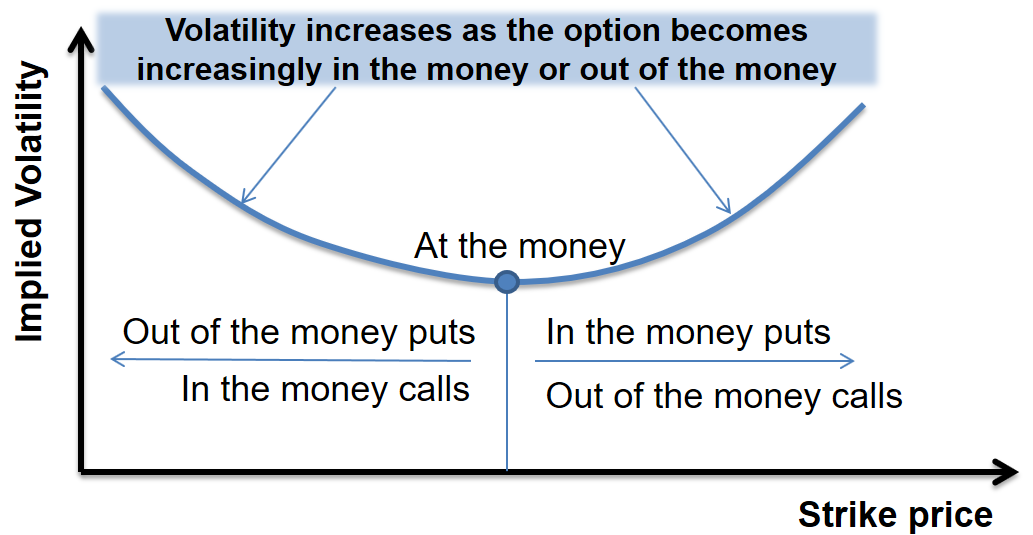
\includegraphics[width=0.8\textwidth]{fig/volatility-smile.png}
    \caption{波动率微笑}
    \label{fig:volatility-smile}
\end{figure}

\subsection{波动率微笑与波动率偏斜}

波动率微笑(Volatility smile)定义为期权的隐含波动率与在值程度(K/S或K/F)的曲线。或可以定义为隐含波动率与期权Delta之间的关系,在这样定义下,一般将平值期权定义为$\text{Delta}=0.5$的看涨期权,或$\text{Delta}=-0.5$的看跌期权,这些平值期权一般称为“50-delta期权”(50-delta options)。

波动率微笑的不同取决于,资产的隐含分布:
\begin{itemize}
    \item 若为标准正态分布(只有一、二阶矩),则应为一条直线
    \item 若三阶矩有负偏(右偏),则投资者预期未来标的资产将大幅下跌概率大,则波动率微笑此时为一条斜向下的曲线,称为波动率偏斜(Volatility skew);若三阶矩为正偏(左偏),则变为斜向上的曲线
    \item 若四阶矩存在尖峰肥尾,则波动率微笑为对称,两侧向上弯曲的曲线,为波动率微笑
\end{itemize}

\begin{figure}[H]
    \centering
    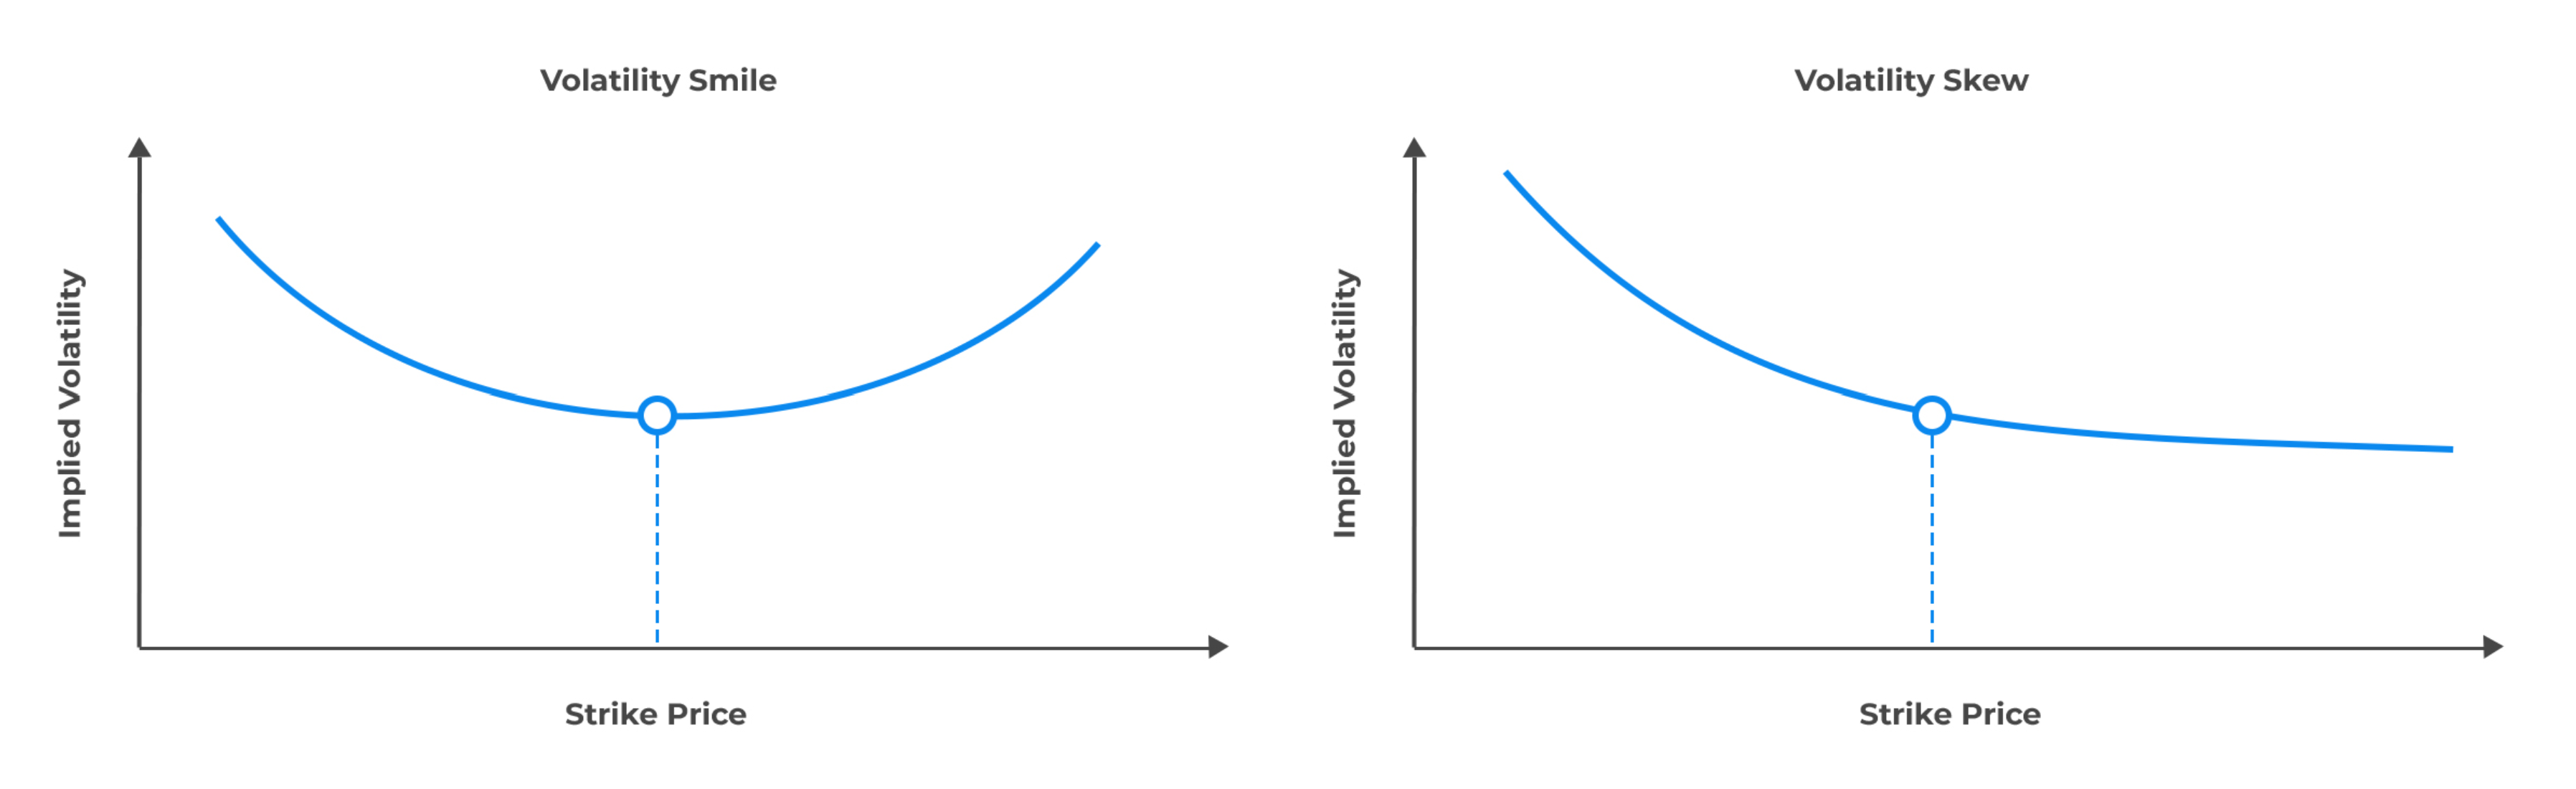
\includegraphics[width=0.9\textwidth]{fig/volatility-smile-skew.png}
    \caption{波动率微笑与波动率偏斜}
    \label{fig:volatility-smile-skew}
\end{figure}

\subsection{波动率微笑与隐含风险中性分布}

通过在某一时刻到期的波动率微笑,可以确定这一时间的资产价格风险中性分布,将这一分布称之为\uline{隐含概率分布}(Implied distribution)\footnote{见OFOD第十版第20章、章节末附录20A与Breeden and Litzenberger (1978)}

对于期限为$T$、执行价格为$K$的欧式看涨期权的价格应为如下所示。其中$r$为利率,假定为常数,$g$为$S_T$:
\begin{equation*}
    c = e^{-rT} \int_{S_T=K}^{\infty} \left( S_T - K \right) g(S_T) dS_T
\end{equation*}

此时如果对$K$求导,可以得到:
\begin{align*}
    \frac{\partial c}{\partial K} &= -e^{-rT} \int_{S_T=K}^{\infty} g(S_T) dS_T \\
    &= -e^{-rT} \bigg[ G(S_T) \bigg]_{K}^{\infty} \\
    &= -e^{-rT} \left[ G(\infty) - G(K) \right] \\
    &= e^{-rT} \left[ G(K) - G(\infty) \right]
\end{align*}

进一步对$K$求导:
\begin{align*}
    \frac{\partial^2 c}{\partial K^2} &= \frac{\partial }{\partial K} \left[ e^{-rT} G(K) - e^{-rT} G(\infty) \right] \\
    &= e^{-rT}g(K)
\end{align*}

此时,概率密度函数$g$则:
\begin{equation*}
    g(K) = e^{rT} \frac{\partial^2 c}{\partial K^2}
\end{equation*}

这样就可以使用波动率微笑来估计风险中性概率分布。假定$c_1$、$c_2$和$c_3$为期限为$T$,执行价格为$K-\delta$、$K$和$K+\delta$的看涨期权,并假定$\delta$较小,因此可得到近似:
\begin{align*}
    g(K) &\approx e^{rT} \left[ \frac{c_1+c_3-2c_2}{\delta^2} \right] \\
    &= e^{rT} \left[ \frac{c(K-\delta,T)+c(K+\delta,T)-2c(K,T)}{\delta^2} \right]
\end{align*}

\section{波动率曲面}

\subsection{样条插值}

使用最广泛的为样条插值(Spline interpolation),具体而言,为使用称之为\textbf{样条}的特殊分段多项式(Piecewice polynomial)进行插值。使用样条插值可以有效避免龙格现象(Runge's phenomenon),按照多项式次数,可分为线性(一次)样条插值(即数据点用直线进行连接)、二次样条插值、三次样条插值。对于三次样条插值(Cubic spline interpolation)要求函数值,一阶导数,二阶导数都连续(节点左右值相等)。而当使用的三次多项式形式为埃尔米特(Hermite)多项式时,又称之为三次埃尔米特样条插值(Cubic Hermite interpolation),要求节点(knots)值与一阶导数值相等。

假设对于带插值的$n$节点$x_0,x_1,\dots,x_n$,其中端点(End points)为$x_0,x_n$。可分为$n$个区间,假设区间内的样条函数为$S_1,\dots,S_n$。限制端点或数据点导数,或对其他条件进行限制,又可将三次样条插值方法进行如下划分:
\begin{itemize}
    \item 钳制三次样条(Clamped cubic spline):限制端点的一阶导数值为任意值,即$S_{1}^{'}(x_0)=v_0$与$S_{n}^{'}(x_{n})=v_n$
    \item 自然三次样条(Natural cubic spline):要求端点的二阶导数为零,即$S_{1}^{''}(x_0)=0$与$S_{n}^{''}(x_{n})=0$
    \item 曲率调整三次(Curvature-adjusted cubic spline):端点的二阶导数不为零,为任意选择值,即$S_{0}^{''}(x_0)=v_0$与$S_{n}^{''}(x_{n})=v_n$
    \item 非扭结三次样条(Not-a-knot cubic spline):不限制端点的导数,但限制除端点之外的第一个节点$x_1$,与最后一个节点$x_{n-1}$两侧样条函数的三阶导数相等,即$S_{1}^{'''}(x_1) = S_{2}^{'''}(x_{1})$与$S_{n-1}^{'''}(x_{n-1}) = S_{n}^{'''}(x_{n-1})$
    \item 抛物线终结的三次样条(Parabolically terminated cubic spline):第一段与最后一段的样条函数,$S_1$与$S_n$的次数被限制在最高二次
\end{itemize}

另外有贝塞尔曲线(Bezier curves),为使得可以节点的导数值可以控制的样条,但作为牺牲,节点处的一阶与二阶导数的平滑性不再能保证,有线性贝塞尔曲线、二次贝塞尔曲线,三次贝塞尔曲线。B样条(B-spline)或称为基样条(Basis spline),为贝塞尔曲线的一般化,可进一步推广为非均匀有理B样条(Non-Uniform Rational B-Splines,NURBS)。

\begin{remark}
    Python库

    在python中可使用\verb|scipy.interpolate.CubicSpline|进行插值
\end{remark}

\subsection{其他方法}

在Carr和Wu(2020)中,采用了Independent bivariate Gaussian kernal的方法。

\section{远期(期货)}

\subsection{定价}

定价思路为由于在签订远期合约时,有双方公平的原则(Zero net market value at entry),应有$f(0,S_0)=0$,即远期合约签订之时为价值0。从而得到远期(期货)价格$F_{t,T}$,即在t时刻,使得远期合约价值为零的合理交割价格。
\begin{itemize}
    \item $S_t$:远期(期货)标的资产在t时刻的价格
    \item $K$:远期合约中的交割价格(Delivery price)
    \item $f(t,S_t)$:远期合约在t时刻的价值(合约价格)
    \item $F_{t,T}$:在t时刻时,到期时间为T的理论远期(期货)价格(标的物价格)
\end{itemize}

\subsubsection{风险中性定价}

对于\textbf{远期合约},其持有人在到期日T必须支付签订合约时约定的交割价格K,购买一份标的资产股票现货,此时远期合约的价值为$S_T-K$。在风险中性条件下,t时刻一份远期(期货)合约的价值$f_t(t,S_t)$应为:
\begin{align*}
    f(t,S_t) &= e^{-r(T-t)} \rnE[S_T - K] \\
    &= e^{-r(T-t)} \rnE(S_T) - e^{-r(T-t)} K \\
    &= S_t - e^{-r(T-t)} K
\end{align*}

在签订之时基于双方公平的原则,应有合约在签订$t=0$之时,远期合约的价值应为0。因此可以确定合理的交割价格$K_{\text{fair}}$,即为合理的远期价格$F_{0,T}$:
\begin{equation*}
    f(0,S_0) = S_0 - e^{-rT}K = 0
\end{equation*}

此时合理的交割价格$K_{\text{fair}} = F_{0,T} = S(0) e^{rT}$。\textbf{远期价格}的定义为在t时刻,使得远期合约价值为0的交割价格。因此在t时刻,远期价格与现货价格之间的关系应为:
\begin{equation*}
    \boxed{
        F_{t,T} = S_t e^{r(T-t)}
    }
\end{equation*}

\subsubsection{复制定价}

假设投资者在$t=0$时刻出售了一份远期合约,为了自我保护,该投资者可以建立一个\textbf{静态对冲}。由远期合约在T时刻的价值为$S_T - K$可知,可分为两部分,一部分为股票市场,一部分为货币市场。该需要在$t=0$时刻,购买一份股票$S_0$,并且从货币借入$e^{-rT}K$,之后不进行任何交易。到到期日期,股票账户为$S_T$,而货币市场账户负债达到$K$,此时头寸正好为$S_T-K$,为远期合约的价值。且由于该投资者可以在任意$t$时刻建立价值为$S_t - e^{r(T-t)}K$的投资组合,复制远期合约的支付。因此应有远期合约在t时刻价值为:
\begin{equation*}
        f(t,S_t) =  S_t - e^{-r(T-t)} K
\end{equation*}

由于远期价格的定义为,使得远期合约为0的交割价格K。因此远期价格为$F_{t,T} = S_t e^{r(T-t)}$,可以发现远期价格$F_{t,T}$与现货价格$S_t$之间仅相差货币时间价值,这部分货币的时间价值可理解为持有成本。因购买远期不占用资金,无资金成本(假设保证金也会获得相应占用资金无风险利息)。相反购买现货则需要占用资金,应支付相应的无风险利息作为其持有成本,无套利条件使得无论购买现货或远期都应有相同成本。因此有远期价格大于现货价格,否则如果购买远期与现货价格相同,那么所有人会直接购买远期,节约购买现货的资金持有成本。

\subsection{红利资产调整}

由于持有远期合约并不实际持有股票,因此无法获得股票在到期前支付的红利,并且股票进行分红后,需要对股价进行除息处理,股票价格回落。将现货价格$S_t$进行调整,剔除其中红利影响,使调整后标的资产变为无红利资产,并以此计算远期价格,得到有红利的股票价格与其远期价格的关系。可以从两个方向进行理解:股票价格回落,自然远期价格也应回落;并且由于远期并不获得红利,因此也应下调远期价格。

另外对于股指期货与股指而言,也需要进行红利调整。股票除息都会提前公布,若发生在股指期货合约期限内,由于股指因股价除息而自然回落是在未来,且是必然事件,那么期货价格就应该对这一合约期内的未来事件进行调整。

\subsubsection{已知红利}
远期合约到期之前,标的资产产生红利数额为$D$,其红利现值为$I_t$,则有$S_t-I_t$为剔除红利,使其变为无红利资产。此时远期价格$F_{t,T}$为使得远期合约价值为零的交割价格K:
\begin{equation*}
    f(t,S_t) = \left( S_t - I_t \right) - K e^{-r(T-t)} = 0
\end{equation*}

则对于已知红利资产,其调整红利后的价格应为:
\begin{equation*}
    F_{t,T} = \left(S_t - I_t \right)e^{r(T-t)}
\end{equation*}

\begin{itemize}
    \item \textbf{正红利}:附息债券(Coupon bond)、支付已知现金红利的股票。价格中包含红利,购买期货无法获得这部分收益,应从中扣除。
    \item \textbf{负红利}:黄金、白银,持有期间需要支付储藏成本。价格中不包含需要额外支付成本,可理解为如果黄金现货和期货价格相同,而黄金期货不需要储藏成本,那么所有人会直接购买黄金期货,所以在购买期货应加上这部分储藏成本,否则可以进行套利。
\end{itemize}

\subsubsection{已知红利率}

同样由于持有远期合约并不实际持有现货,若在远期合约到期期间,标的资产会产生与现货价格成一定比率为$q$的红利,应剔除。或理解为由于期货不享受到分红,因此只愿意出比原价格更低的价格:
\begin{equation*}
    f(t,S_t) = S_t e^{-q(T-t)} - K e^{-r(T-t)} = 0
\end{equation*}

因此对于已知红利率$q$的资产,其调整之后的价格应为:
\begin{equation*}
    F_{t,T} = S_t e^{(r-q)(T-t)}
\end{equation*}

\begin{itemize}
    \item 外汇远期和期货:外汇发行国的无风险利率
    \item 股指期货:市场平均红利率或零,取决于股指计算方式
    \item 远期利率协议:本国的无风险利率
\end{itemize}

\subsection{\tops{$F_{t,T}$}与\tops{$S_t$}}

如上部分讨论,对于对于无红利股票远期与现货,有$F_{t,T} = S_t e^{r(T-t)}$,由于持有股票的持仓成本即为占用资金的成本。而对于大宗商品等则需要考虑持仓成本,在t时刻,远期(期货)价格$F_t$与现货价格$S_t$有如下关系,易知持仓成本即将现货持有到期的成本,否则将可进行套利。由于远期为合约,只在规定到期日交割标的资产。在合约到期之前并不持有实际现货,因此无法获得持有现货的收益,并且持有现货到合约到期日的成本需计算在远期价格内,两者关系应有如下关系。其中对于商品期货,便利收益指实际持有持有现货带来的收益,一般认为由于持有现货有两点优势:可从短期商品的紧缺中获利,也可保持生产线的运转。
\begin{align*}
    F_{t,T} &= S_t + \textbf{净持仓成本(Net cost of carry)} \\
    &= S_t + \text{合约期限内成本(Carry cost)} - \text{合约期限内收益(Carry return)} \\
    &= S_t + \text{利息成本} + \text{储藏成本(storage cost)} - \text{红利收益} - \text{便利收益(Convenience yield)}
\end{align*}

由于在$t$时刻,如现货价格和持仓成本都为已知,则可确定期货价格。相反已知期货的价格与持仓成本,则可确定现货价格,此为期货的价格发现功能。两者为相对价格关系,基于无套利条件得到。在中国往往有现货价格$S_t$大于期货价格$F_t$(期货贴水,此时有正基差),即现货价格被高估。这是由于现货做空机制不完善,很难进行融券,即使能融券成本也较高。使得套利投资者无法在现货被高估的情况下,通过卖出现货(卖出开仓)买进期货(因为只有持有现货才能卖出)进行套利。造成现货与期货市场的分割,无法达到一体化的预期。另外由于买卖现货需要交纳印花税,而期货不需要,且期货佣金往往低于现货。

\subsubsection*{基差与期货升贴水}

基差(Basis)指现货与远期价格之差(现货价格Spot price有时又被称为Cash price)。\textbf{注意}:如在万得中定义基差为期货价格减去现货价格。在此定义下,“负基差”指现货价格高于期货价格。如上式$F_t$与$S_t$的关系可知,现货价格高于期货价格,期货处于贴水状态,此时净持仓成本为负。
\begin{equation*}
    \textbf{基差} = \text{现货价格} - \text{期货价格}
\end{equation*}

对于远期(期货)而言,\textbf{升水}(contango)指当期货价格高于现货价格(或未来预期即期价格),此时为期货溢价,此时有负基差。也称为正向市场(Normal market),即期限较短的合约(Near-maturity contract)价格低于期限较远的合约(Far-maturity contract)。相反而言,如期货价格低于现货价格,则称期货\textbf{贴水}(Backwardation),此时为现货溢价,有正基差。或称为逆向市场(Inverted market),即期限较短合约的价格高于期限较远的合约。

需要注意的是,与商品期货相反,\uline{在金融期货中,一般定义基差为期货价格减去现货价格}。因此,当金融期货贴水,称有负基差,而金融期货,称有正基差。

\begin{figure}[H]
    \centering
    \begin{tikzpicture}
        \draw[->,thick] (0,0) node[below]{$t$} -- (4,0) node[below]{时间} -- (9,0);
        \draw[->,thick] (0,0)--(0,5) node[above]{价格};  
        \draw[dashed, draw opacity=0.6] (8,0) node[below]{到期日} -- (8,4.5);
        \draw[decorate, decoration = {snake,segment length=2em,amplitude=1mm}] (0,0.5) node[left,xshift=-1em]{\small $F_{t,T}$贴水} -- (8,2.5) node[midway,above,sloped]{\small 逆向市场};
        \draw[decorate, decoration = {snake,segment length=2em,amplitude=1mm}] (0,2.5) node[left,xshift=-1em]{\small $S_t$} -- (8,2.5);
        \draw[decorate, decoration = {snake,segment length=2em,amplitude=1mm}] (0,4.5) node[left,xshift=-1em]{\small $F_{t,T}$升水} -- (8,2.5) node[midway,above,sloped]{\small 正向市场};
        \draw[decorate,decoration={brace,amplitude=5pt,mirror,raise=0.2em}] (0,0.5) -- (0,2.5) node[midway,right,xshift=0.6em]{\small 正基差};
        \draw[decorate,decoration={brace,amplitude=5pt,mirror,raise=0.2em}] (0,2.5) -- (0,4.5) node[midway,right,xshift=0.6em]{\small 负基差};
    \end{tikzpicture}
    \caption{$F_{t,T}$与$S_t$}
\end{figure}

\subsection{\tops{$F_{t,T}$}与\tops{$\E_t[S_T]$}}

在现实测度下,两者应相差风险溢价,但由于风险溢价的不确定性,因此两者关系并不确定:
\begin{equation*}
    F_{t,T}=\E[S_T]-\text{风险溢价}
\end{equation*}

从现货角度出发,在现实测度下设$\mu$为到期收益率,则应有$\E_t[S_T]=S_t e^{\mu(T-t)}$,此时$\mu$为无风险收益率与风险溢酬之和。如果标的资产$S$\textbf{系统性风险为正},则要求有\textbf{正的风险溢酬}。在T时刻,假设期货价格$S_T = F_{T,T}$为2000,标的资产的系统风险为正,对持有者不利,则要求500元的正的风险溢价为承担风险的补偿,此时$S_t$为1500元。则有到期收益率大于无风险收益率$\mu>r$,因为承担额外的风险需要额外的风险溢酬作为回报。

\begin{figure}[H]  
    \centering
    \begin{subfigure}[b]{0.5\textwidth}
    \begin{tikzpicture}[scale=0.9]
        \draw[->,thick] (0,0) node[below] {$t$} -- (6,0) node[below] {时间};  
        \draw[->,thick] (0,0) -- (0,4) node[above] {价格};  
        \draw (4.5,0) node[below] {$T$} -- (4.5,4);
        \draw [draw opacity=0.6](0,0.5) node[left] {$S_t$} -- (4.5,2.5) node[right] {$\E_t[S_T]$}; 
        \draw [draw opacity=0.6](0,1.5) node[left] {$F_{t,T}$} -- (4.5,2.5);
        \draw [dashed, draw opacity=0.6] (0,2.5) -- (4.5,2.5);  
        \draw [dashed, draw opacity=0.6] (0,0.5) -- (4.5,0.5);  
        \draw [decorate,decoration={brace,amplitude=5pt,mirror,raise=0.2em}] (0,0.5) -- (0,1.5) node[midway,right,xshift=0.6em]{\small r};
        \draw [decorate,decoration={brace,amplitude=5pt,mirror,raise=0.2em}] (0,1.5) -- (0,2.5) node[midway,right,xshift=0.6em]{\small 正风险溢酬};
        \draw[decorate,decoration={brace,amplitude=5pt,raise=0.2em}] (4.5,0.5) -- (4.5,2.5) node[midway,left,xshift=-0.6em]{\small $\mu$};
    \end{tikzpicture}
    \subcaption{正系统性风险} 
    \label{fig:M1}  
    \end{subfigure}%
    \begin{subfigure}[b]{0.5\textwidth}
    \begin{tikzpicture}[scale=0.9]
        \draw[->,thick] (0,0) node[below] {$t$} -- (6,0) node[below] {时间};  
        \draw[->,thick] (0,0) -- (0,4) node[above] {价格};  
        \draw (4.5,0) node[below] {$T$} -- (4.5,4);
        \draw [draw opacity=0.6](0,0.5) node[left] {$S_t$} -- (4.5,2.5) node[right] {$\E_t[S_T]$}; 
        \draw [draw opacity=0.6](0,3.5) node[left] {$F_{t,T}$} -- (4.5,2.5);
        \draw [dashed, draw opacity=0.6] (0,2.5) -- (4.5,2.5);
        \draw [dashed, draw opacity=0.6] (0,0.5) -- (4.5,0.5);  
        \draw [decorate,decoration={brace,amplitude=5pt,raise=0.2em}] (0,0.5) -- (0,3.5) node[midway,left,xshift=-0.6em]{\small r};
        \draw [decorate,decoration={brace,amplitude=5pt,mirror,raise=0.2em}] (0,2.5) -- (0,3.5) node[midway,right,xshift=0.6em]{\small 负风险溢酬};
        \draw[decorate,decoration={brace,amplitude=5pt,raise=0.2em}] (4.5,0.5) -- (4.5,2.5) node[midway,left,xshift=-0.6em]{\small $\mu$};
    \end{tikzpicture}
    \subcaption{负系统性风险}
    \label{fig:M2}  
    \end{subfigure}
    \caption{现实测度下$F_{t,T}=S_t e^{r(T-t)}$与$\E(S_T)$}
\end{figure}  

相反,如果标的资产$S$\textbf{系统性风险为负}(如VIX系统性风险为负),则应有\textbf{负的风险溢酬}。即标的资产能对冲风险,减少风险敞口,此时风溢酬为负,减少收益,使得到期收益率小于无风险收益率$\mu<r$。

从期货角度出发,同样在现实测度下,因为购买期货无需占用资金(假设保证金可获得无风险收益),所以不要求无风险收益。仅要求对其承担的未来不确定性风险,有对应的风险补偿,收益率为$\mu-r$,可以得到$\E_t[F_{T,T}] = F_{t,T} e^{(\mu-r)(T-t)}$。期货到期日T时刻,有期货价格等于现货价格$F_{T,T} = S_T$,即在t时刻下也应有两者期望$\E_t[F_{T,T}] = \E_t[S_T]$。另外虽然现货价格可以从市场交易信息中得到,但由于期货市场交易成本较低,反应较为灵敏迅速,价格变化一般都由期货市场传递至现货市场。在t时刻,期货与现货以及其现实测度期望关系如下图所示:

\begin{figure}[H]  
    \centering
    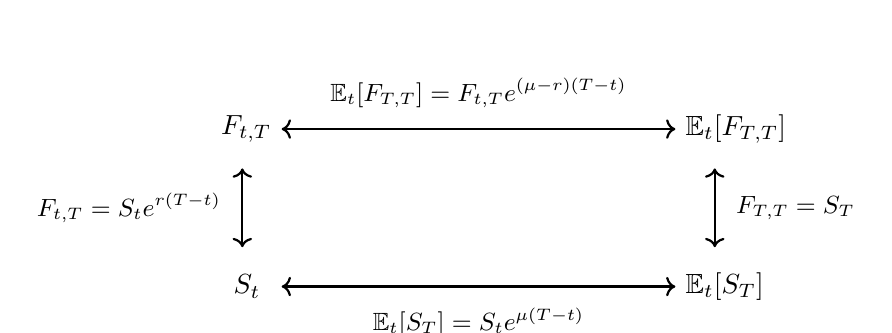
\begin{tikzpicture}
        \draw [<->,thick] (1,0) node [left,xshift=-0.4em]{$S_t$} -- (6,0) node [right]{$\E_t[S_T]$} node [midway,below,yshift=-0.4em]{\small $\E_t[S_T] = S_t e^{\mu(T-t)}$};
        \draw [<->,thick] (1,2) node [left]{$F_{t,T}$} -- (6,2) node [right]{$\E_t[F_{T,T}]$} node [midway,above,yshift=0.4em]{\small $\E_t[F_{T,T}] =F_{t,T} e^{(\mu-r)(T-t)}$};
        \draw [<->,thick] (0.5,0.5) -- (0.5,1.5) node [midway,left,xshift=-0.4em]{\small $F_{t,T}=S_t e^{r(T-t)}$};
        \draw [<->,thick] (6.5,0.5) -- (6.5,1.5) node [midway,right,xshift=0.4em]{\small $F_{T,T}=S_T$};
    \end{tikzpicture}
    \caption{现货期货以及现实测度期望关系}
\end{figure}

\section{远期(期货)套期保值}

完美套期保值
\begin{itemize}
    \item 远期(期货)的到期日、标的资产和交易金额等条件的设定使得远期(期货)与现货正好匹配
    \item 完全消除价格风险
\end{itemize}

不完美套期保值
\begin{itemize}
    \item 常态
    \item 无法完全消除价格风险
\end{itemize}

\subsection{基差风险}

如前文定义,基差为现货价格$H$(被套期保值对象)与期货价格$G$(套期保值工具)的价差,即$b = H - G$,未来基差的不确定性导致了\textbf{基差风险}。由于标的资产规模与期货合约标准数量之间的差异,导致了\textbf{数量风险}。基差风险、数量风险都可能使得套期保值策略无法对冲所有风险,即不完美的套期保值。

\uline{多头套期保值策略}持有现货空头,担心未来价格上涨,买入期货锁定未来价格(期货多头)。由于价格上涨,期货多头获利,即称之为多头策略。相反,\uline{空头套期保值策略}持有现货多头,担心未来价格下跌,卖出期货锁定未来卖出价格(期货空头)。以下表\ref{tab:basis-risk}为例,收益分为现货收益与期货收益两部分:

\begin{table}[H]
\centering
\begin{tabular}{@{}cll@{}}
\toprule
\multicolumn{1}{l}{}           
& \multicolumn{1}{c}{\textbf{多头套期保值}} & \multicolumn{1}{c}{\textbf{空头套期保值}} \\
\midrule
\textbf{初始仓位} & 1单位现货空头,1单位期货多头 & 1单位现货多头,1单位期货空头 \\
\textbf{基差收益} &$\quad(H_0 - H_1) + (G_1 - G_0)$ & $\quad(H_1 - H_0) + (G_0 - G_1)$ \\
& $=(H_0 - G_0) - (H_1 - G_1)$ & $=(H_1 - G_1) - (H_0 - G_0)$ \\
& $=b_0 - b_1$ & $=b_1 - b_0$ \\
\textbf{收益来源} & 基差变小 $b_0>b_1$ & 基差变大 $b_0<b_1$\\
\multirow{3}{*}{\textbf{收益条件}} & 1. 现货涨幅小于期货涨幅 & 1. 现货涨幅大于期货涨幅 \\
& 2. 现货跌幅大于期货跌幅 & 2. 现货跌幅小于期货跌幅 \\ 
& 3. 现货价格下跌而期货价格上涨 & 3. 现货价格上涨而期货价格下跌 \\
\bottomrule
\end{tabular}
\caption{多头与空头套期保值}
\label{tab:basis-risk}
\end{table}

$b_0$已知,由此可知未来时刻基差$b_1$决定了是否能完美套期保值。当现货价格小于期货价格时,期货升水,基差为负。假设$b_0=-10$,多头套保策略要有正收益要求基差变小,即$b_0>b_1$,$b_0=-10$,则有$b_1< -10$。\uline{注意此时虽然基差变小,但基差的绝对值在增大。}

若期货标的与现货标的不同,假设期货标的的价格为$S$,那么可以将如上未来时刻基差$b_1$进行分解:
\begin{equation*}
    b_1 = H_1 - G_1 = (S_1 - G_1) + (H_1 - S_1)
\end{equation*}

可以看到等式右边第一项为未来时刻期货与其标的现货的基差$S_1 - G_1$,由于日期不一致,可能导致两者不同。第二项为由于期货标的与现货不同$H_1 - S_1$,即出现在交叉套期保值的情况下,现货价格的差异,这两者原因都可能造成无法实现完美的套期保值。

\subsection*{逼仓}

对于进行交割的期货而言,期货多方容易进行逼仓,由于期货为合约,且多方为动用资金,资金容易筹集,用于购买现货。若有大量未平仓合约,即空方要交割大量现货,大多时候现货数量有限,且有各种运输储存成本,难以筹集,因此造成没有足够的现货供应,造成了\uline{逼空}的产生。

同样\uline{逼多}也有可能发生,即虽然资金容易筹集,但也需要有进行实务交割的能力,若多方完全不具备接收实物的能力,只能进行平仓,使得原油价格快速下跌(原油宝事件)。

【待考证】

\subsection{套保(金额)比率}

套期保值比率(Hedge Ratio),指现有头寸(金额)中,已有多少被套期保值(对冲)。假设当前有1000元的现货头寸,其中600元已使用期货进行套期保值,表示当前套期保值比率为0.6或60\%,同时表示还留有风险敞口40\%。
\begin{equation*}
   \text{套期保值(金额)比率} = \frac{\text{套期保值资产头寸}}{\text{被套期保值资产头寸}}
\end{equation*}

\subsection{套保(数量)比率}

在已知了目前风险暴露情况,即套保(金额)比率之后,还希望了解在现有的现货头寸(被套保资产)之下,需要多少数量的期货进行对冲。希望在期货到期时,最大化消除被套保资产价格变动所带来风险。

此时要求被套保资产价格的变动对整个组合价值影响最小,进而转化为求解最小值问题。即对$\Delta H$求偏导,并使一阶条件$\partial\Delta\Pi / \partial \Delta H = 0$,求得\textbf{最优套期保值(数量)比率n}(价格无法控制,只能控制数量)。因只关注最终期货到期时刻的套保比率,而不关注过程中的套保比率,所以此处使用的是$\Delta H$而非$\partial H$。

对于多头套期保值组合,有:
\begin{align*}
    &\Delta \Pi = n\Delta G - \Delta H \\
    &\Rightarrow\quad\frac{\partial (\Delta \Pi)}{\partial (\Delta H)}  = n\times \frac{\partial (\Delta G)}{\partial (\Delta H)} - 1 = 0 \\ 
    &\Rightarrow \quad n = \frac{\partial(\Delta H)}{\partial(\Delta G)} = \frac{\partial r_H \times H_0}{\partial r_G \times G_0} 
\end{align*}

对于空头套期保值组合,同样有:
\begin{align*}
    &\Delta \Pi = \Delta H - n \Delta G \\
    &\Rightarrow\quad\frac{\partial (\Delta \Pi)}{\partial (\Delta H)}  =  1 - n\times \frac{\partial (\Delta G)}{\partial (\Delta H)} = 0 \\ 
    &\Rightarrow \quad n = \frac{\partial(\Delta H)}{\partial(\Delta G)} = \frac{\partial r_H \times H_0}{\partial r_G \times G_0} 
\end{align*}

对多头套期保值或空头套期保值均有最优套保比率$n=\partial(\Delta H)/\partial(\Delta G)$,$r_H$和$r_G$为H与G在套期保值期间的收益率。n代表期货价格变动一个单位,现货价格变化多少,同时代表\textbf{每单位数量现货需要n单位数量期货进行对冲}。因现货与期货为线性关系,即套期保值后不需要随时间调整两者之间比率n,此为\textbf{静态套保(Static Hedge)}。与之相反的为\textbf{动态套保(Dynamic Hedge)},需要不断随时间调整两者之间比率。

得知每单位数量现货需要n单位期货进行对冲之后,根据持有现货H头寸数量$Q_H$,可计算出需要多少份(手)的期货G合约进行对冲。即可求得最优套期保值(期货)合约份数N,使得期货总价值变动等于持有现货总价值变动。
\begin{align*}
    N = n \times \frac{Q_H}{Q_G} = \frac{\partial(\Delta H)\times Q_H}{\partial(\Delta G)\times Q_G} = \frac{\partial(r_H \times H_0 \times Q_H)}{\partial(r_G \times G_0 \times Q_G)} = \frac{\partial r_H \times V_H}{\partial r_G \times V_G}
\end{align*}

由$n \times Q_H$计算得到,对于现有头寸$Q_H$单位数量的现货,需要多少单位数量的期货进行对冲。再除以$Q_G$期货合约规模(乘数),计算得到需要N份(手)期货合约进行对冲。此时$V_H$为被套期保值的所持有现货资产总价值,而$V_G$则为每份期货合约价值(单位价格$\times$合约乘数)。\textbf{注意:n代表的是单位数量,而N为份数(手),为最小买卖单位。如螺纹钢期货报价单位为元/每吨,一份合约(手)包含10单位数量(吨)期货,即合约规模(乘数)为10。}

\subsection{最小方差套保(数量)比率}

当将风险定义为方差时,最优的套保比率可定义为,使套期保值组合收益$\Delta\Pi$方差最小的套期保值(数量)比例n,即为\textbf{最小方差套保比率}。$\sigma_\Pi^2$为套期保值组合收益的方差,对$n$求导,使一阶条件为零,二阶条件$d^2(\sigma_H^2)/dn^2=2\sigma_G^2>0$,有最小值。对于多头套保组合或空头套保组合,其最小方差套期保值比一般公式为:
\begin{align*}
    \sigma_{\Pi}^2 &= \sigma_H^2 + n^2\sigma_G^2 - 2n\sigma_{HG}\\
    &\Rightarrow \quad \frac{d\sigma_\Pi^2}{dn} = 2n\sigma_G^2 - 2\sigma_{HG} = 0 \\
    &\Rightarrow \quad n = \frac{\sigma_{HG}}{\sigma_G^2} =\rho_{HG} \frac{\sigma_H}{\sigma_G}
\end{align*}

其中$\sigma_H = \sigma_{\Delta H}$,$\sigma_G = \sigma_{\Delta G}$,$\sigma_{HG}$为$\Delta H$与$\Delta G$的协方差,$\rho_{HG}$为$\Delta H$与$\Delta G$的相关系数($\rho_{XY} = Cov(X,Y)/\sigma_X\sigma_Y$)。我们可以进而推导出基于收益率的最小方差套期保值比率,首先:
\begin{align*}
    \rho_{HG} &= \frac{Cov(\Delta H,\Delta G)}{\sqrt{Var(\Delta H)} \sqrt{Var(\Delta G)}} \\
    &= \frac{Cov(r_H \times H_0,r_G \times G_0)}{\sqrt{Var(r_H \times H_0)} \sqrt{Var(r_G \times G_0)}}\\
    &= \frac{H_0 G_0 Cov(r_H,r_G))}{H_0 \sqrt{Var(r_H)} \times G_0 \sqrt{Var(r_G)}} \\
    &= \frac{Cov(r_H,r_G)}{\sqrt{Var(r_H)} \sqrt{Var(r_G)}} = \rho_{r_H r_G}
\end{align*}

其次:
\begin{equation*}
    \frac{\sigma_H}{\sigma_G} =  \frac{\sqrt{Var(r_H \times H_0)}}{\sqrt{Var(r_G \times G_0)}} = \frac{H_0 \sqrt{r_H}}{G_0 \sqrt{r_G}} = \frac{\sigma_{r_H} H_0}{\sigma_{r_G} G_0}
\end{equation*}

因此有:
\begin{equation*}
    n = \rho_{r_H r_G}\frac{\sigma_{r_H} H_0}{\sigma_{r_G} G_0}
\end{equation*}

\subsection{OLS估计}
可以观察$n = Cov(\Delta H,\Delta G)/Var(\Delta G),$即为OLS回归中的系数$b$。则可用OLS回归,估计$b$:
\begin{equation*}
    \Delta H = a + b\Delta G + \varepsilon
\end{equation*}

需注意套保期限与回归中使用的$\Delta H$和$\Delta G$的期限应相同,即如果要锁定未来一个月的现货价格,需使用现货和期货的月价格变化进行回归。且调整后得到实际需要套期保值(期货)合约份数N为:
\begin{equation*}
    N =  b \frac{Q_H}{Q_G}
\end{equation*}

也可使用收益率进行OLS回归估计,且在时间极短时,百分比收益率$\Delta P/P$与对数收益率可视为相等。且对数收益率更符合平稳序列和正态分布的假设,在平稳假设的下对每日现货和期货的对数收益率进行回归:
\begin{equation*}
    r_H = a + b'r_G + \varepsilon
\end{equation*}

此时:
\begin{align*}
    b &= \frac{Cov(\Delta H,\Delta G)}{Var(\Delta G)} \\ 
    &= \frac{Cov(r_H \times H_0,r_G \times G_0)}{Var(r_g \times G_0)} \\
    &= \frac{H_0G_0 Cov(r_H,r_G)}{G_0^2 Var(r_G)} \\
    &= b'\frac{H_0}{G_0}
\end{align*}

对应需套期保值合约份数N(手):
\begin{equation*}
    N =  b\frac{Q_H}{Q_G} = b'\frac{H_0 \times Q_H}{G_0 \times Q_G} = b'\frac{V_H}{V_G}
\end{equation*}

\subsection{风险降低百分比}

通过检验风险降低百分比,可以检验使用最小方差套期保值比率的套期保值效果。将最小方差套期保值比率$n = \rho_{HG}\frac{\sigma_{H}}{\sigma_{G}}$,带回套期保值组合方差$\sigma_{\Pi}^2 = \sigma_H^2 + n^2\sigma_G^2 - 2n\sigma_{HG}$中。可以得到:
\begin{equation*}
    e^* = \frac{\sigma_{H}^2 - \sigma_{\Delta \Pi}^2}{\sigma_{\Delta H}^2} = \rho_{HG}^2
    =\frac{Cov^2(\Delta H, \Delta G)}{Var(\Delta H)Var(\Delta G)}
    =\frac{Cov^2(r_H H_0, r_G G_0)}{Var(r_H H_0)Var(r_G G_0)}
    =\rho_{r_Hr_G}^2
\end{equation*}

而在一元线性回归中判别系数$R^2=\rho$,即回归效果越好,$R^2$越接近1,套期保值的效果也越好。

\section{看跌-看涨平价关系(欧式期权)}

看跌-看涨期权平价关系(Put-call parity),指具有相同的行权价与到期日的欧式看涨期权与欧式看跌期权,其价格之间存在的关系。若平价关系不成立,则意味着存在套利的空间。现实市场中存在交易成本,又如在中国市场现货无法自由做多做空,因此买卖权平价关系不完全成立。然而欧美市场等流动性较好的市场中,可以近似认为买卖权平价关系成立。

PCP平价可以直接从BS公式中推导;
\begin{align*}
    C_{t,T} &= P_{t,T} + S_t -K \\
    S_t N(d_1) - K e^{-r(T-t)} N(d_2) &= K e^{-r(T-t)} N(-d_2) - S_t N(-d_1) S_t -Ke^{-r(T-t)} \\
    &= K e^{-r(T-t)} [1- N(d_2)] - S_t [1 - N(d_1) ] + S_t -Ke^{-r(T-t)} \\
    &= \cancel{K e^{-r(T-t)}} - K^{-r(T-t)} N(d_2) - \cancel{S_t} + S_t N(d_1) + \cancel{S_t} - \cancel{K^{-r(T-t)}} \\
    &= C_{t,T}
\end{align*}
也可以看到,相同行权价到期时间的看涨看跌期权,两者波动率应该相等,否则PCP平价不成立。

\subsection{无红利资产}

\subsubsection*{使用现货}

对于无红利资产,使用股票(不支付股息),构建如下两个组合,且看涨期权与看跌期权具有相同的执行价格$K$与期限$T$:
\begin{itemize}
    \item 组合A:欧式看涨多头 + 在$T$时刻收益为$K$的零息债券
    \item 组合B:欧式看跌多头 + 1股股票
\end{itemize}

在T时刻,投资组合A与B有:
\begin{table}[H]
\centering
\begin{tabular}{@{}clll@{}}
\toprule
                     &   & $S_T>K$ & $S_T<K$ \\ \midrule
\multirow{3}{*}{组合A} & 看涨期权 & $S_T-K$ & $0$ \\
                    & 零息债券 & $K$ & $K$ \\
                    & 总和   & $S_T$ & $K$ \\ \midrule
\multirow{3}{*}{组合B} & 看跌期权 & $0$ & $K-S_T$ \\
                     & 股票   & $S_T$ & $S_T$ \\
                     & 总和   & $S_T$ & $K$ \\ \bottomrule
\end{tabular}
\end{table}

根据无套利原理,在$T$时刻两个组合有相同的收益,因此在$t$时刻也必须有相同的价值,否则就可以进行套利。零息债券在$t$时刻现值为$Ke^{-rT}$,因此可以得到:
\begin{equation*}
    C_{t,T} + Ke^{-r(T-t)} = P_{t,T} + S_t
\end{equation*}

\subsubsection*{使用远期}

对于无红利资产,使用远期合约(适用于中国市场与美国市场),构建如下两个组合,且看涨期权与看跌期权具有相同的执行价格$K$与期限$T$:
\begin{itemize}
    \item 组合A:欧式看涨多头
    \item 组合B:欧式看跌多头 + 远期合约多头
\end{itemize}

在T时刻,投资组合A与B有:
\begin{table}[H]
\centering
\begin{tabular}{@{}clll@{}}
\toprule
                     &   & $S_T>K$ & $S_T<K$ \\ \midrule
\multirow{3}{*}{组合A} & 看涨期权 & $S_T-K$ & $0$ \\
                    & 总和   & $S_T-K$ & $0$ \\ \midrule
\multirow{3}{*}{组合B} & 看跌期权 & $0$ & $K-S_T$ \\
                     & 远期合约 & $S_T-K$ & $S_T-K$ \\
                     & 总和   & $S_T-K$ & $0$ \\ \bottomrule
\end{tabular}
\end{table}

可以发现在T时刻,两种情况之下A、B两个投资组合的收益相同:
\begin{equation*}
    C(T,S_T) = P(T,S_T) + f(T,S_T)
\end{equation*}

并且根据无套利原则,在任意t时刻两个投资组合的价值也必须相同,否则将存在套利机会:
\begin{equation*}
    C(t,S_t) = P(t,S_t) + f(t,S_t)
\end{equation*}

将远期合约在$t$时刻价值$f(t,S_t) = S_t - Ke^{-r(T-t)}$代入,则有对于现货价格的PCP公式有:
\begin{equation*}
    C_{t,T} = P_{t,T} +  S_t - K e^{-r(T-t)}
\end{equation*}

利用市场上观察到的看涨看跌期权价格,可求出隐藏现货价格。在中国市场中现货无法做空,可以用期权价格计算隐含现货价格:
\begin{equation*}
    S^*_t = \left( C_{t,T} - P_{t,T} \right) + K e^{-r(T-t)}
\end{equation*}

或使用期货,则有远期合约在$t$时刻价值$f(t,F_t) = (F_{t,T} - K) e^{-r(T-t)}$,可得到对于远期(期货)的PCP公式:
\begin{equation*}
    C_{t,T} = P_{t,T} + \left( F_{t,T} - K \right) e^{-r(T-t)}
\end{equation*}

同样利用市场上已知的看涨看跌期权价格,可求得隐藏期货价格:
\begin{equation*}
    F^*_{t,T} = \left( C_{t,T} - P_{t,T} \right) e^{r(T-t)} + K
\end{equation*}

\subsection{有红利资产}

对于在到期日T之前支付已知红利的标的资产,设支付红利现值为$I_t$,则应有调整后的远期价格为$F_{t,T} = (S_t - I_t)e^{r(T-t)}$,因此调整后的PCP公式有:
\begin{equation*}
    C_{t,T} = P_{t,T} + S_t - I_t - Ke^{-r(T-t)}
\end{equation*}

同理,对于已知红利率资产,设红利率为$q$,调整后的远期价格为$F_{t,T} = S_t e^{(r-q)(T-t)}$,因此有调整后的PCP公式为:
\begin{equation*}
    C_{t,T} = P_{t,T} + S_t e^{-q(T-t)} - Ke^{-r(T-t)}
\end{equation*}

\subsection{中国市场PCP}

在中国市场中,由于标的资产无法自由做多做空,因此现货PCP关系不完全成立。远期可以做多也可以做空,因此远期PCP关系成立,其中远期交割价格等于看涨与看跌期权的行权价,期限相同:
\begin{equation*}
    C_{t,T} = P_{t,T} + \left( F_{t,T} - K \right) e^{-r(T-t)}
\end{equation*}

目前中国市场中所拥有的金融衍生品与其标的资产如下:
\begin{table}[H]
\centering
\begin{tabular}{@{}cccc@{}}
\toprule
\textbf{金融衍生品}    & \textbf{现货}          & \textbf{期货} & \textbf{期权} \\ \midrule
\textbf{股指(中金所)}  &                      & 上证50股指期货    &             \\
\textbf{}         &                      & 沪深300股指期货   & 沪深300股指期权   \\
\textbf{}         &                      & 中证500股指期货   &             \\
\textbf{ETF(上交所)} & 华夏上证50ETF(510050)    &             & 上证50ETF期权   \\
\textbf{}         & 华泰柏瑞沪深300ETF(510300) &             & 沪深300ETF期权  \\
\textbf{ETF(深交所)} & 沪深300ETF(159919)     &             & 沪深300ETF期权  \\ \bottomrule
\end{tabular}
\end{table}

在中国市场中,如上表所示,相同标的的股指期货与期权,或ETF现货与期权之间可以使用PCP关系而不做调整。对于ETF而言,ETF成分股分红,分红会留存在ETF之内。50ETF以及300ETF现货进行分红,期权则会进行相应调整,因此ETF现货与其期权,均受到红利保护,因此不需要调整红利,可视为无红利资产使用PCP关系式。

而对于股指期货而言,指数根据成分股价格加权计算得出,在到期日之内成分股分红,股指将自然回落,不做任何调整,因此股指期货无红利保护。对于沪深300股指期权与股指期货,为同一标的,虽然不受红利保护,但两者之间的PCP也不需要进行调整。可由远期与期权PCP关系计算,如使用股指期权估算隐含远期价格,不需要进行红利调整。注意:与股指期货与股指不同,股指期权与股指期货同时对期限内未来的除息进行调整,因此两者之间不需要进行调整。

ETF有红利保护,ETF远期(中国市场未上市)无红利保护,因此建立两者之间的PCP关系式则需要调整红利。已知$F_{t,T} = (S_t - I_t)e^{r(T-t)}$,将其代入现货PCP公式可得下列关系式。可理解为由于远期无红利保护,而ETF期权有红利保护,应将远期加上分红,调整为有分红资产:
\begin{equation*}
    C_{t,T} = P_{t,T} + \left( F_{t,T}-K \right) e^{-r(T-t)} + I_t
\end{equation*}

利用如上PCP关系式,则可以使用ETF期权计算出隐藏ETF远期价格:
\begin{equation*}
    F^*_{t,T} = \left( C_{t,T} - P_{t,T} \right) e^{r(T-t)} + K - I_t e^{r(T-t)}
\end{equation*}

\subsection{ETF期权分红调整}

对于股票股利,由于股票稀释,因此需要进行\textbf{除权}(XR,Ex-Right)调整。若配股比例为$25/1000$为1000股配25股,假设拥有1000股的股东,持有股票数目变为$1025$。为了保持公司总市值不变,因此需要进行除权,将市场每股价格等比例下调,做法为将除权日前一天收盘价除以$1+25/1000$。而对于现金股利,则称之为\textbf{除息}(XD,Ex-Dividend)。做法为将除息日前一天的收盘价对应减去现金股利。

交易所之所以会在分红后进行期权合约调整,是因为ETF分红后期权买卖双方的权利义务大小会相应变化。核心的问题是如何通过调整来维持期权合约买卖双方权利义务的均衡。一般来说,期权合约调整有两个目标:
\begin{itemize}
    \item 调整后,合约行权成本(行权价格$\times$合约单位)不变
    \item 调整后,合约市值(结算价格$\times$合约单位)不变
\end{itemize}

\divider

根据《上海证券交易所股票期权试点交易规则》第三章第十三条,对合约标的除权、除息的,期权合约的合约单位、行权价格按照下列公式进行调整:
\small
\begin{equation*}
    \textbf{新合约单位} = \frac{\text{原合约单位}\times\left(1+\text{流通股份实际变动比例}\right)\times\text{除权(息)前一日合约标的收盘价}}{\left(\text{除权(息)前一日合约标的收盘价格}-\text{现金红利}\right)+\text{配股价格}\times\text{流通股份实际变动比例}}
\end{equation*}
\begin{equation*}
    \textbf{新行权价格} = \frac{\text{原行权价格}\times\text{原合约单位}}{\text{新合约单位}}
\end{equation*}
\normalsize

调整后的合约单位,按照四舍五入的原则取整数;调整后的行权价格,按照四舍五入的原则取小数,合约标的为股票的,保留两位小数,合约标的为交易所交易基金的,保留3位小数。

\divider

\begin{example}

华夏上证50ETF

根据510050管理人华夏基金2020年11月11日发布《上证50交易型开放式指数证券投资基金利润分配公告》,2020年11月27日为基金分红的权益登记日,11月30日为基金分红的除息日,分红发放日为12月03日,方案为每十份510050基金分红为0.51元,对象为登记日下午交易结束后所有基金份额持有人。根据交易规则,权益登记日下一交易日,即除息日进行除息除权处理。交易所利用前收盘价,计算除权除息参考价格,作为除息日开盘价(集合竞价产生)的参考。在此例子中27日不复权收盘价3.557,前复权收盘价为3.506,为调整了分红后的收盘价(决定涨跌幅)。

上交所于11月11日同日,发布公告将于2020年11月30日对50ETF期权合约的行权价格、合约单位、合约交易代码和合约简称进行调整,并对除息后的50ETF新挂2020年12月、2021年1月、3月和6月等4个月份的标准化合约。已知510050前一个交易日11月27日周五收盘价为3.557元/份,分红金额为每份分红0.051元,流通股份实际变动比例为0,可计算50ETF期权合约的新合约单位为:
\begin{equation*}
    \text{新合约单位} = 10000 \times \frac{3.557}{3.557-0.051} = 10145
\end{equation*}

使用公式计算合约“50ETF购2020年12月3000”新行权价格:
\begin{equation*}
    \text{新行权价格} = \frac{10000}{10145} \times 3.000 = 2.957
\end{equation*}

根据新计算的行权价格,将原合约新挂为“50ETF购2020年12月2957A”。并由于行权价的下调,使得期权买卖双方的权利义务重新平衡。期权合约“50ETF购2020年12月3000”的于27日结算价为0.5616元,由如下公式计算该期权合约30日调整后前结算价(决定保证金):
\begin{equation*}
    \text{新结算价格} = \frac{\text{原结算价格}\times\text{原合约单位}}{\text{新合约单位}} = \frac{10000}{10145} \times 0.5616 = 0.5536
\end{equation*}

可以看到期权合约对于分红的调整有如下几步,先根据ETF27日(除息日30日前一交易日)的收盘价及分红调整合约单位,其实质为缩放比例,为分红调整之后价格与分红之前价格比值的倒数。再根据新合约单位(缩放比例),等比例缩小行权价格与结算价格。合约单位比例放大与价格比例缩小相互抵消,使得合约行权与实际市值保持不变。

\end{example}

\divider

在处理这类数据时需要额外注意:
\begin{itemize}
    \item 跨过除夕日的合约,会自动变为带A的合约,代表已经经过调整。如上所述,其行权价$K$与合约单位都已经过调整。在事后时间点看,这些合约都会带上A,在事前进行计算时需要调整回原有的行权价与合约单位
    \item 一般使用不带A的进行计算,而且也有可能出现调整后的带A的期权行权价,与正常期权行权价正好重合的情况
    \item 对于\verb|510050.OF|而言,从2015-02-09期权上市之后,其除息日有(上交所期权同一日进行除息处理):
    \begin{itemize}
        \item 2016-11-29
        \item 2017-11-28
        \item 2018-12-03
        \item 2019-12-02
        \item 2020-11-30
        \item 2021-11-29
    \end{itemize}
\end{itemize}
注意:在处理数据时,

\subsubsection*{关于结算价格}

上交所在每个交易日收盘后向市场公布期权合约的结算价格,作为计算期权合约每日日终维持保证金、下一交易日开仓保证金、涨跌停价格等数据的基准。

原则上,期权合约的结算价格为该合约当日收盘集合竞价的成交价格。但是,如果当日收盘集合竞价未形成成交价格,或者成交价格明显不合理,那么上交所就会考虑期权交易的多重影响因素,另行计算合约的结算价格。即根据同标的、同到期日、同类型其他行权价的期权合约隐含波动率,推算该合约隐含波动率,并以此计算该合约结算价。

此外,期权合约最后交易日如果为实值合约的话,由上交所根据合约标的当日收盘价格和该合约行权价格,计算该合约的结算价格;期权合约最后交易日如果为虚值或者平值合约的话,结算价格为0。

期权合约挂牌首日,以上交所公布的开盘参考价作为合约前结算价格。合约标的出现除权、除息的,合约前结算价格按照以下公式进行调整:新合约前结算价格=原合约前结算价格×(原合约单位/新合约单位)。除权除息日,以调整后的合约前结算价作为涨跌幅限制与保证金收取的计算依据。

\section{中国市场特殊处理}

在中国市场存在理论与实务脱节的问题。主要有卖空限制导致现货价格高估,内在价值与时间价值,与平值点定义需要更改。解决同一行权价到期期限的看涨看跌波动率相差大;解决隐含波动率为0;看跌期权时间价值明显高于看涨期权的时间价值;期权时间价值为负;平值点时间价值不是最大等问题。

\textbf{关于无套利与可复制}:无套利指当套利机会出现,人们会利用套利机会获利,使得套利机会消失,表达的是人的主观意愿的假设。而可复制表达是是否能利用套利机会,表达是市场环境是否能允许套利进行。如现货价格被高估,期货价格被低估,虽然人们愿意进行套利,但在中国市场由于现货卖空存在限制,所以难以复制,最终导致了套利无法进行,无套利不满足。

\subsection{做空限制与隐含信息}

在中国市场中,现货市场存在较大的做空限制,使得市场中的价格由所以看多者和少量看空者决定,看空者的情绪无法表达,因此并不能反应所有投资者的真实情绪,现货价格相对被高估。现货由于卖空限制,难以复制并进行套利,违法BSM假设中允许卖空标的证券的条件。若使用现货价格进行隐含信息的计算存在较大误差,主要解决方法为从衍生品市场取得隐含现货期货价格。
\begin{enumerate}
    \item 使用BSM公式,从衍生品市场提取隐含合理的现货价格:
    \begin{itemize}
        \item \uline{期货}中隐含的现货价格(无红利资产):
        \begin{equation*}
            S^*_t = F_{t,T} e^{-r(T-t)}
        \end{equation*}
        \item \uline{ETF期权}中隐含的现货价格,虽然ETF有红利但期权会进行调整,可视为无红利资产:
        \begin{equation*}
            S^*_t = \left( C_{t,T} - P_{t,T} \right) + Ke^{-r(T-t)}
        \end{equation*}
        \item \uline{股指期权}中隐含的现货价格(已知红利率),成分股分行股指不做调整自然回落,则有:
        \begin{equation*}
            S^*_t = \left( C_{t,T} - P_{t,T} \right)e^{q(T-t)} + Ke^{-(r-q)(T-t)}
        \end{equation*}
    \end{itemize}
    \item 使用Black公式,从衍生品市场提取隐藏合理的期货价格:
    \begin{equation*}
        F^*_{t,T} = \left(C_{t,T} - P_{t,T}\right) e^{r(T-t)} + K
    \end{equation*}
\end{enumerate}

由衍生品市场得到隐含的现货价格$S^*_{t}$与隐含的期货价格$F^*_{t,T}$,就可以使用对应的BSM公式或Black公式,计算其隐含波动率。对于平价期权的确定一般选用价格最接近,即看涨看跌期权价差最小的一组期权作为平价期权。

\subsection{内在价值}

已知期权价值可分解为内在价值(Intrinsic value)与时间价值(Time value)两个部分,即:
\begin{equation*}
    \boxed{
        \text{期权价值} = \text{内在价值} + \text{时间价值}
    }
\end{equation*}

以波动划分,内在价值为\textbf{不考虑资产价格波动}的情况下,期权条款赋予期权多头的最高价值。而时间价值为\textbf{标的资产价格波动}为期权多头(权利方)所带来的隐含价值,由于期权的权利方只有权力而无义务,因此期权的内在价值以及时间价值都应大于0。时间价值受内在价值的影响,但内在价值不受时间价值的影响,因而使用两分法。即先计算出期权的内在价值,使用二分法,再确定期权的时间价值。

\subsubsection{John Hull定义}

定义内在价值为,期权若在当下时点到期,期权所含的的内在价值,如OFOD教科书、上交所、万得中。若美式期权,这样定义就是合理的,由于美式期权在到期日之前可以随时行权,则其内在价值都基于当前时点的股价与行权价进行计算。但如果是欧式期权,则没有考虑行权价货币的时间价值,现货价格为当前时点,但行权价为未来时点,应该对未来时点的行权价进行贴现。且在中国市场由于现货的卖空限制,其实际价格被高估。
\noindent\begin{align*}
    \text{看涨期权内在价值} & = \max(S_t-K,0) \\
    \text{看跌期权内在价值} & = \max(K-S_t,0)
\end{align*}

期权的内在价值与时间价值关系如下,可以看到下边界为当标的资产价格趋近于零时,看涨期权趋近于S,下边界为$\max(S-K,0)$:
\begin{figure}[H]
    \centering
    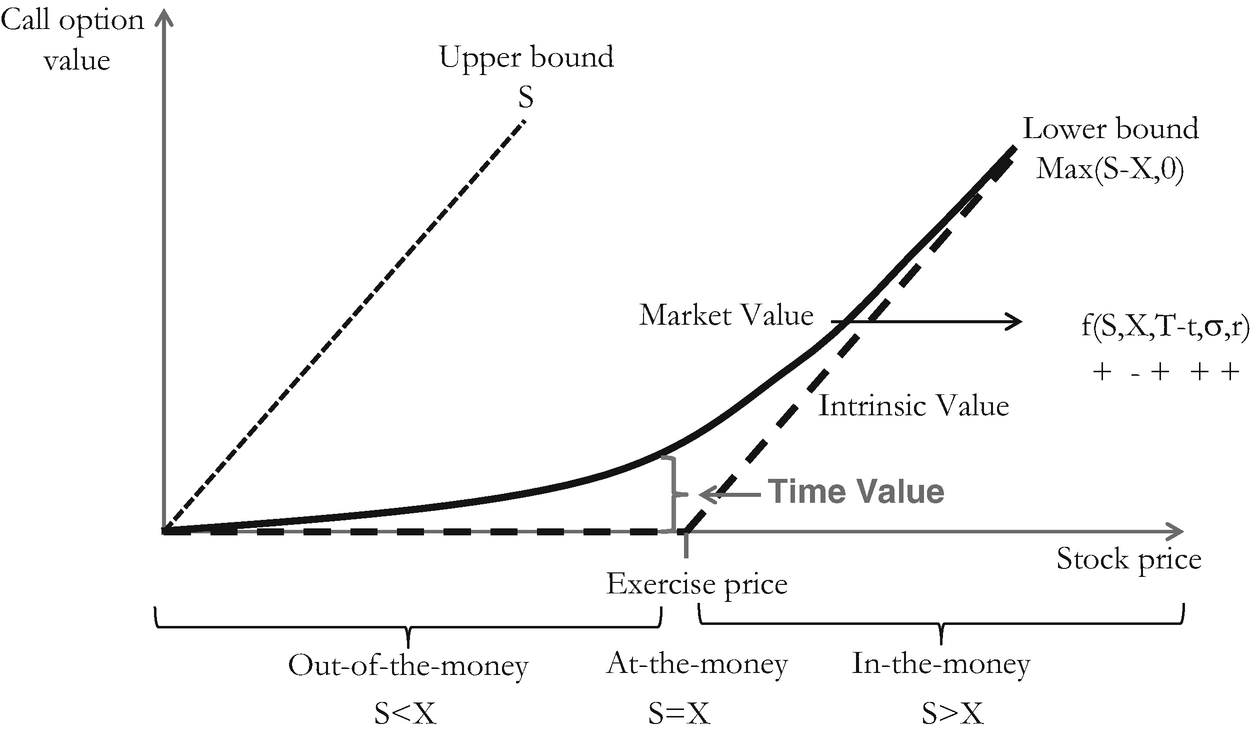
\includegraphics[width=0.8\textwidth]{fig/call-vs-stock.png}
    \caption{看涨期权价格与标的价格}
    \label{fig:call-vs-stock}
\end{figure}

\subsubsection{完美市场定义}

在考虑货币时间价值的情形内在价值如下,在完美市场中可适用,但没有考虑中国市场的卖空限制,需要进一步进行调整。
\begin{align*}
    \text{看涨期权内在价值} & = \max\left(S_t-Ke^{-r(T-t)},0\right) \\
    \text{看跌期权内在价值} & = \max\left(Ke^{-r(T-t)}-S_t,0\right)
\end{align*}

\subsubsection{中国市场定义}

不考虑时间价值,那么欧式看涨权利方与远期合约多头的差别就是期权只有权利而没有义务,因此内在价值应为$\max(f_{t,T},0)$。同理,对于欧式看跌期权应有$\max(-f_{t,T},0)$。即使用期货价格代替现货价格,在期货市场多空双方均能自由表达其看法,且中美市场均可使用,因此有:
\begin{align*}
    \text{看涨期权内在价值} & = \max\left[(F_{t,T}-K)e^{-r(T-t)},0\right] \\
    \text{看跌期权内在价值} & = \max\left[(K-F_{t,T})e^{-r(T-t)},0\right]
\end{align*}

\subsubsection{ETF期权股指期货定义}

由于在中国市场ETF期权,如50ETF,有红利保护机制。即会下调行权价格,放大每手期权数量,相当于变相抬高了股票价格进行复权,修复由于分红带来的影响,因此可视为无红利资产进行处理。而在中国市场中并没有50ETF期货,只有股指期货,且股指期货不对分红进行调整,即没有红利保护,即其成分股分红后股指自然下跌。因此使用股指期货计算ETF期权内在价值时,还需要再做红利调整。由于在计算期货时将现货中的红利剔除:
\begin{equation*}
    F_{t,T} = ( S_t - I_t )e^{r(T-t)}
\end{equation*}

因此,在计算内在价值时应将剔除的红利加回:
\begin{align*}
    \text{看涨期权内在价值} & = \max\left[ (F_{t,T}-K) e^{-r(T-t)} + I_t \right] \\
    \text{看跌期权内在价值} & = \max\left[ (K-F_{t,T}) e^{-r(T-t)} - I_t \right]
\end{align*}

\subsection{平值点与在值程度}

平值点是使得期权内在价值由正值变化到零(内在价值非负)的临界行权价,因为平值点使得内在价值变为零,则平值点使用远期价格的定义应为$F_{t,T}=K$,这样的定义使得实值虚值部分左右较为对称,利于比较,具体参考郑和陈(2018)与郑、杨与阮(2021)。

同理,对于现货(中国市场使用隐含现货价格)而言,平值点应有:
\begin{itemize}
    \item 无红利:$S_t e^{r(T-t)}$
    \item 有红利:$\left(S_t - I_t \right)e^{r(T-t)} $
    \item 红利率:$S_t e^{(r-q)(T-t)}$
\end{itemize}

使用对数在值程度(Log-moneyness)作为在值程度的定义,优点是使得值域范围有$(-\infty,\infty)$,使得实值期权与虚值期权幅度上对称。
\begin{equation*}
    \ln \frac{K}{K_{\text{ATM}}} = \ln \frac{K}{F}
\end{equation*}

同时可以发现,根据PCP公式:
\begin{equation*}
    C_{t,T} = P_{t,T} + \left( F_{t,T} - K \right) e^{-r(T-t)}
\end{equation*}

根据平值期权ATM定义有$F_{t,T}=K$,易得此时$C_{t,T}=P_{t,T}$。

当$F_{t,T} \geq K$时,此时看涨期权ITM,同时具有内在价值与时间价值。而看跌期权OTM,因此只具有时间价值。由如上定义,此时看涨期权内在价值为$\left( F_{t,T} - K \right) e^{-r(T-t)}$。根据PCP可以看到:
\begin{align*}
    C_{t,T} &= P_{t,T} + \left( F_{t,T} - K \right) e^{-r(T-t)} \\
    \cancel{C_{\text{内在价值}}} + C_{\text{时间价值}}
    &= P_{\text{时间价值}} + \cancel{C_{\text{内在价值}}} \\
    C_{\text{时间价值}} &= P_{\text{时间价值}}
\end{align*}

同理,当$F_{t,T}<K$时,看跌期权为实值,同时具有内在价值与时间价值。因此,在新平值点定义下,\textbf{相同行权价、相同期限的看涨期权与看跌期权的时间价值应该相等}。

\section{平价期权估计}

当平值点为$S_t = K e^{-r(T-t)}$时,将其带入看涨BSM公式当中,则有:
\begin{equation*}
    \frac{C}{S} = N(d_1) - N(d_2)
\end{equation*}

同样,对于看跌期权则有:
\begin{align*}
    \frac{P}{S} & = N(-d_2) - N(-d_1) \\
    & = 1 - N(d_2) - [1-N(d_1)] \\
    & = N(d_1) - N(d_2) = \frac{C}{S}
\end{align*}

也可用期货价格进行改写,即$\frac{C}{Fe^{-r(T-t)}}$与$\frac{P}{Fe^{-r(T-t)}}$。对于$d_1$和$d_2$,此时有:
\begin{align*}
    d_1 &= \frac{\ln(S/K)+(r+\sigma^2/2)(T-t)}{\sigma\sqrt{T-t}} = \frac{\sigma}{2}\sqrt{T-t} \\
    d_2 &= \frac{\ln(S/K)+(r-\sigma^2/2)(T-t)}{\sigma\sqrt{T-t}} = d_1 - \sigma\sqrt{T-t}= -\frac{\sigma}{2}\sqrt{T-t}
\end{align*}

则对于欧式平价看涨或看跌期权,有看涨与看跌期权价格相等,将期权价格记为$V$:
\begin{align*}
    \frac{V}{S} &= N \left( \frac{\sigma\sqrt{T-t}}{2} \right) - N\left( -\frac{\sigma\sqrt{T-t}}{2} \right) \\
    & = N \left( \frac{\sigma\sqrt{T-t}}{2} \right) - N\left( -\frac{\sigma\sqrt{T-t}}{2} \right) \\
    & = 2N\left( \frac{\sigma\sqrt{T-t}}{2} \right) - 1
\end{align*}

对于正态分布有CDF:
\begin{equation*}
   N(x) = \int \frac{1}{\sqrt{2\pi}} e^{-\frac{1}{2}x^2} dx
\end{equation*}

已知对于自然指数$e^x$,其泰勒展开有:
\begin{equation*}
    e^x = \sum^{\infty}_{n=0} \frac{x^n}{n!} = 1 + x + \frac{x^2}{2!} + \frac{x^3}{3!} + \dots
\end{equation*}

替换将$x$替换为$-\frac{x^2}{2}$:
\begin{equation*}
    e^{-\frac{x^2}{2}} = 1 -\frac{x^2}{2}  + \frac{x^4}{8} - \frac{x^6}{48} + \dots
\end{equation*}

使用泰勒展开,将正态分布的自然指数替换:
\begin{align*}
   G(x) &= \frac{1}{\sqrt{2\pi}} \int e^{-\frac{x^2}{2}} dx \\
   &= \frac{1}{\sqrt{2\pi}} e^{-\frac{1}{2}} \int \left( 1 -\frac{x^2}{2}  + \frac{x^4}{8} - \frac{x^6}{48} + \dots \right) dx \\
   &= \frac{1}{\sqrt{2\pi}} \left( x -\frac{x^3}{6} + \frac{x^5}{40} - \frac{x^7}{336} + \dots \right) 
\end{align*}

注意在求泰勒展开的积分之后,还需要加上常数项$C$,因此应有:
\begin{equation*}
    N(x) = G(x) + C
\end{equation*}

已知对于标准正态分布CDF,$N(0) = G(0) + C = \frac{1}{2}$,因此$C=\frac{1}{2}$,即:
\begin{equation*}
   N(x) = \frac{1}{2} + \frac{1}{\sqrt{2\pi}} \left( x -\frac{x^3}{6} + \frac{x^5}{40} - \frac{x^7}{336} + \dots \right) 
\end{equation*}

令$x=\frac{\sigma\sqrt{T-t}}{2}$代入上式,则对于欧式平价期权:
\begin{align*}
    \frac{V}{S} & = 2N\left( \frac{\sigma\sqrt{T-t}}{2} \right) - 1 \\
    & = 2\left[\frac{1}{2} + \frac{1}{\sqrt{2\pi}} \left(\frac{\sigma\sqrt{T-t}}{2} - \frac{(\sigma\sqrt{T-t}/2)^3}{6} + \frac{(\sigma\sqrt{T-t}/2)^5}{40} - \dots + \dots\right) \right] - 1\\
    &\approx \frac{\sigma\sqrt{T-t}}{\sqrt{2\pi}} \approx 0.4\sigma\sqrt{T-t}
\end{align*}

\section{可转债}


\appendix

\begin{appendices}

\section{牛顿迭代法}

牛顿迭代法(Newton's method)又称为牛顿-拉弗森方法(Newton-Raphson method),是一种迭代估计方程根的算法。

\subsection{\tops{$f(x)$}的根}

对于函数$y = f(x)$,使用泰勒公式进行展开
\begin{equation*}
    f(x) = f(x_0) + f'(x_0)(x-x_0) + \frac{1}{2}f''(x_0)(x-x_0)^2 + \dots + \frac{1}{n!}f^{(n)}(x_0)(x-x_0)^n
\end{equation*}

保留前两项,并令$f(x) = 0$,即有:
\begin{equation*}
    f(x) = f(x_0) + f'(x_0)(x-x_0) = 0
\end{equation*}

整理上式,当$f'(x_0) \neq 0$时应有:
\begin{equation*}
    x = x_0 - \frac{f(x_0)}{f'(x_0)}
\end{equation*}

迭代可得令$f(x) = 0$的根:
\begin{equation*}
    x_{t+1} = x_t - \frac{f(x_t)}{f'(x_t)}
\end{equation*}

\begin{remark}
    原理为,先取任意一点$x_0$,根据$f(x_0)$与其切线$f'(x_0)$,可计算出切线与$x$轴相交与点$x_1$。同样根据$f(x_1)$与$f'(x_1)$,可以计算出切线与$x$轴相交于$x_2$,不断迭代,即可求得函数$f(x)=0$的根。
\end{remark}

\subsection{\tops{$f'(x)$}的根}

同理,对于$f'(x)$的根,使用泰勒公式,并保留前三项:
\begin{equation*}
    f(x) = f(x_0) + f'(x_0)(x-x_0) + \frac{1}{2}f''(x_0)(x-x_0)^2
\end{equation*}

对等式两边求导可得:
\begin{equation*}
    f'(x) = 0 + f'(x_0) + \frac{1}{2}f''(x_0)*2(x-x_0)
\end{equation*}

同理,令$f'(x) = 0$可得:
\begin{equation*}
    f'(x) = f'(x_0) + f''(x_0)(x-x_0) = 0
\end{equation*}

当$f''(x_0) \neq 0$应有:
\begin{equation*}
    x = x_0 - \frac{f'(x_0)}{f''(x_0)}
\end{equation*}

迭代可得令$f'(x) = 0$的根:
\begin{equation*}
    x_{t+1} = x_t - \frac{f'(x_t)}{f''(x_t)}
\end{equation*}


\section{股指计算方法}

\subsection{道琼斯}
    
道琼斯工业平均指数(Dow Jones Industrial Average, DJIA),计算方法为成分股的平均值,除以一个Dow Divisor。
\begin{equation*}
    \text{DJIA} = \frac{\sum P_i }{\text{Divisor}}
\end{equation*}

其中Divisor用于调节,当股票拆分、分拆之等,又如旧公司退出,新公司进入,使得指数保持不变。可以看到这样编制的缺点就是每支成分股都等权重的编入股指,假设A公司或B公司上涨10元,那么都将导致股指将上涨10。但若A公司的流通股数量是B的10倍,显然影响远超B公司。

\subsection{标准普尔500}

标准普尔500指数(Standard \& Poor's 500,S\&P 500) ,标普500是使用市值作为权重计算指数,称为Capitalization-weighted indices,简称market cap weighted,或称为Value-weighted。
\begin{equation*}
    \text{SP 500} = \frac{\sum P_{i,1} Q_{i,0}}{\sum P_{i,0}, Q_{i,0}}
\end{equation*}

大致编制方法为,标普500对于每个公司都计算Investable Weight Factor或IWF,用于计算可供投资者交易的$Q$,即$Q=\text{IWF}_i * \text{Total shares}_i$,用于去除掉不流通股票,这样也称为float-adjusted,分母为该成分股编入股指时的价格。

\section{汇率表示方法}

USD/JPY约为136,即1美元兑换136日元。USD/CNY约为6.7,即美元兑人民币为6.7,从字面理解即1美金,兑换6.7人民币,也可称为CNY per USD。也经常表示为USDCNY或USD:CNY,称为USD to CNY或USD against CNY。在前的货币称为Base currency,在后的称为Quote currency,或称为Local currency。

以做多USD/CNY为例,假设当前为6.7,一个月后上涨至6.8,即每单位USD可兑换的CNY变多,即Base currency USD对CNY上涨,从而获利。若做空USD/CNY,那么希望USD跌。根据做多做空盈利的方向而言,此时Base currency为在外汇交易者买入的货币,而Quote currency为卖出的货币,所持有的希望卖出的货币,所以也称为Local currency。

若将苹果作为一种货币,假设苹果价格为2元/个(苹果)或$\frac{\text{苹果}}{\text{人民币}}= \frac{2}{1}$,即有苹果:人民币为2。做多苹果,那么希望base currency涨价,即苹果涨价。此时人民币为Local currency,即希望卖出的人民币,买入苹果。套用美元兑人民币的例子,同样可以表述为6.7 CNY/USD,此时local currency为人民币,卖出人民币,买入美元。
\begin{equation*}
    \text{USD} : \text{CNY} = 6.7:1 \quad \Rightarrow \quad 1 \text{USD} = 6.7 \text{CNY}
\end{equation*}

或理解为:
\begin{equation*}
    \$1 : \yen 1 = 6.7:1 \quad \Rightarrow \quad  \$ 1 = \yen 6.7
\end{equation*}

即需要6.7元才能买入1美元,或卖出1美元能买入6.7元人民币,两种表述方式相同,但可见Base currency即为每单位或1单位该货币,为基准能兑换N单位其他国家货币。

\section{利率平价}

利率平价(Interest rate parity)可分为以下两种:
\begin{itemize}
    \item Covered Interest Rate Parity(CIP):利用远期合约锁定远期汇率,对冲风险
    \item Uncovered Interest Rate Parity(UIP):不适用远期合约单对冲风险,所以是uncovered,根据有效市场假说,应该不能获得超额收益
\end{itemize}

对于CIP,使用远期汇率对冲风险。假设即期汇率S,远期汇率F(形式均为FOR/LOC,即每单位境外货币FOR,兑换多少LOC当地货币):
\begin{equation*}
    (1 + i_{L}) = \frac{F_{F/L}}{S_{F/L}} (1+ i_{F})
\end{equation*}

两国利差,如中国名义(Nominal)利率为3\%,而美国利率为1\%,那么应该卖出美金,买入人民币,投资中国债券,从而赚取利差。那么未来应该人民币贬值2\%,或美元兑人民币升值2\%,不然就存在套利机会。

从上式变形,等式两边都减去1:
\begin{equation*}
    \frac{(1 + i_{L})}{(1+ i_{F})} - 1 = \frac{i_L-i_F}{1+i_F} = \frac{F_{F/L}}{S_{F/L}} - 1 \\
\end{equation*}

因此对于CIP而言,应有如下关系,即利差与汇率变化相等:
\begin{equation*}
    (i_{L}-i_{F}) \approx \frac{F_{F/L}-S_{F/L}}{S_{F/L}}
\end{equation*}

\begin{example}
    假设当前GBP/USD汇率为1.35,并且美国的利率为1.1\%,英国的利率为3.25\%,那么根据CIP远期汇率应有持有1单位本国货币(USD),$1+1.1\%$。应与1美金兑换成英镑并持有,$\tfrac{1}{S_{F/L}} \times (1+3.25\%)$,最终将其通过远期汇率兑换会美金,两者应有平价关系:
    \begin{equation*}
        (1+1.1\%) = \frac{1}{S_{F/L}} \times (1+3.25\%) \times F_{F/L}
    \end{equation*}

    那么:
    \begin{equation*}
        F_{F/D} = 1.35 \times \frac{(1+1.1\%)}{(1+3.25\%)} \approx 1.32
    \end{equation*}
\end{example}

UIP不适用远期锁定未来汇率,假设UIP成立,未来汇率的期望,应由一下关系得到:
\begin{equation*}
    (1 + i_{L}) = \frac{\E(S_{t+1})}{S_t} (1+ i_{F})
\end{equation*}

若CIP与UIP都同时成立,那么:
\begin{equation*}
    \E (S_{t+1}) = F_{F/L}
\end{equation*}

CIP只需要无套利就能成立,由于交易成本等远远可能违反CIP。


Carry trade:为卖出低利率国家货币,买入高利率国家货币并投资该国

Diversified carry trade:买入一篮子货币


Wikipedia reference:
\begin{itemize}
    \item \href{https://en.wikipedia.org/wiki/Interest_rate_parity}{Interest rate parity}
    \item \href{https://en.wikipedia.org/wiki/Carry_(investment)#Currency}{Carry}
\end{itemize}

\end{appendices}

\end{document}